%%% -*-LaTeX-*-
%%% ====================================================================
%%% This is a sample top-level LaTeX-2e file for typesetting a thesis
%%% or dissertation at the University of Utah.  Most students find it
%%% convenient to start with a COPY of this file as a template, and
%%% then alter that copy to match their needs.
%%%
%%% There is an associated Unix Makefile that can be similarly
%%% customized, and then the only command ever needed to typeset the
%%% complete thesis is the single word "make".  Of course, during
%%% writing and typesetting, not all of the steps are needed, so
%%% often, one can just name a convenience target such as "make
%%% dvi-pass" or "make pdf-pass" to do just a single pass of LaTeX and
%%% BibTeX.
%%%
%%% There should be no, or very few, macro definitions in this file;
%%% any needed belong in a private style file, called mythesis.sty,
%%% and input below after all other packages.  The bulk of this file
%%% should just be command invocations, and any arguments that they
%%% need.
%%%
%%% We exploit the fact that TeX ignores spaces after command names to
%%% line up arguments for better readability.
%%%
%%% Each chapter should be a separate complete file, so that you can
%%% insert a command like \includeonly{chap_intro} before the first
%%% \include{chap_xxx} command to avoid typesetting all but the
%%% chapter that you are currently working on, to save time.
%%%
%%% Remember that occupants of job positions change jobs from time to
%%% time: YOU are responsible for ensuring correct names of all humans
%%% mentioned in this file!
%%%
%%% [16-Mar-2016]
%%% ====================================================================

\documentclass[11pt,Chicago]{uuthesis2e}

%%% Undefine two macros from uuthesis2e.cls that conflict with
%%% definitions in amsthm.sty that fail to check for prior definitions!
%%% NB: The amsthm package refines the LaTeX theorem environment,
%%% and the uuthesis-color-headings wraps that definition, so the
%%% amsthm package must be read first!
\let \proof    = \relax
\let \endproof = \relax
\usepackage {amsthm}

%%% ====================================================================
%%% Choose an alternate font family for the document if the TeX default
%%% of Computer Modern is not wanted:

\usepackage{mathpazo}

%%% ====================================================================
%%% Some miscellaneous Utah- and student-specific settings:
%%%
%%% Chapter is one level, section and subsection are the next two levels.

\fourlevels

%%% ====================================================================
%%% The remaining packages are required by this particular thesis,
%%% but other theses will almost certainly need different packages:
%%%
%%% WARNING: MANY \LaTeX{} packages change dimensions, glue, and/or
%%% formatting styles, and such changes are likely to conflict with
%%% University of Utah Thesis Office requirements.  Therefore, minimize
%%% the number of packages that you include!

\usepackage {amsmath}
\usepackage {amssymb}
\usepackage {bm}
\usepackage {bibnames}
\usepackage {citesort}
\usepackage {graphicx}
\usepackage {graphpap}
\usepackage {longtable}
\usepackage {multirow}
\usepackage {tikz}
\usetikzlibrary {decorations.markings}
\usepackage {varioref}

%%% ====================================================================
%%% Support for a subject index:

%% \usepackage {uuthesis-index}

%%% ====================================================================
%%% The various uuthesis-*.sty packages must come AFTER all other
%%% system-provided packages, so that they can correctly override
%%% settings from those packages.

%%% Include latest updates for 2016 (WARNING: the name is subject to
%%% change: see http://www.math.utah.edu/pub/uuthesis/ for the most
%%% current version.)

\usepackage {uuthesis-2016-h}  % MANDATORY package

%%% This is an OPTIONAL package that sets chapter and sectional headings
%%% in color:
%%% Use one or the other of these:
% \usepackage {color}
%%: \usepackage {uuthesis-color-headings}
%%: \definecolor{utahheadingcolor} {rgb}  {0.7, 0.0, 0.0}
%%: \definecolor{utahtheoremcolor} {rgb}  {0.490,0.149,0.804} % purple4
%%: \definecolor{utahtheoremcolor} {rgb}  {0.545,0.137,0.137} % brown4

%%% Here is another, and more convenient, way to define colors, via
%%% aliases of named colors in the X11-derived rgb.sty file

%%: \usepackage{coloralias}
%%: \definecoloralias{utahheadingcolor}{steelblue4}
%%: \definecoloralias{utahtheoremcolor}{hotpink3}

%%% The default heading color is utahred (defined by University Printing
%%% Services as 0.8 red, 0.0 green, 0.0 blue), but you could redefine
%%% that to, for example, a dark blue color, like this AFTER including
%%% the package:
%%%
%%%     \definecolor{utahheading}{rgb}{0,0,0.8}
%%%
%%% NB: Be careful with use of colors in typesetting, and in figures,
%%% because about 6 percent of the human male population is red/green
%%% color blind: they see those colors as shades of brown.  Red and
%%% blue, or blue and green, are better choices for choosing
%%% distinguishable colors.  Also, avoid light colors, especially
%%% yellow, because they are hard to see against white paper and
%%% screen backgrounds, and when printed on black-and-white printers,
%%% where they are rendered in gray, they may be too faint to read.

%%% ====================================================================
%%% Support for a subject index:
%
%: \usepackage {uuthesis-index}

%%% ====================================================================
%%% This single user-specific file is where all personal customizations
%%% and macro definitions should be placed, and it should come LAST,
%%% after ALL OTHER packages, in case it needs to override some of their
%%% definitions.
\usepackage{url}
\usepackage{graphicx} % Required for inserting images
\usepackage{hyperref}
\usepackage{url}
\usepackage{algorithm}
\usepackage{algpseudocode}
\usepackage{cite}
\usepackage{listings}
\usepackage {mythesis}
\paperwidth=8.5in
\paperheight=11in

\usepackage{xcolor} % For coloring syntax (optional)

\usepackage{lstautogobble}  % Fix relative indenting
\usepackage{color}          % Code coloring
\usepackage{zi4}            % Nice font

\definecolor{bluekeywords}{rgb}{0.13, 0.13, 1}
\definecolor{greencomments}{rgb}{0, 0.5, 0}
\definecolor{redstrings}{rgb}{0.9, 0, 0}
\definecolor{graynumbers}{rgb}{0.5, 0.5, 0.5}

\usepackage{listings}
\lstset{
    autogobble,
    columns=fullflexible,
    showspaces=false,
    showtabs=false,
    breaklines=true,
    showstringspaces=false,
    breakatwhitespace=true,
    escapeinside={(*@}{@*)},
    commentstyle=\color{greencomments},
    keywordstyle=\color{bluekeywords},
    stringstyle=\color{redstrings},
    numberstyle=\color{graynumbers},
    basicstyle=\ttfamily\footnotesize,
    frame=l,
    framesep=12pt,
    xleftmargin=12pt,
    tabsize=4,
    captionpos=b
}
%%% ====================================================================
%%% The student-specific front matter fields are defined here:

\author                 {Hamza Fathallah Al Sheikh}
\title                  {Improving Performance of Multi-Cluster Environments through Trading Mechanisms}
\thesistype             {Thesis}

\dedication             {For my parents, Amal and Youssof.}

%%% Most students need just a short degree name, like this:
\degree                 {Masters of Science \\
                         in \\
                         Computer Science}
%%% However, multiline degrees are possible, and are done like this:
%%% \degree                 {Doctor of Philosophy \\
%%%                         in \\
%%%                         Mathematical Physics}

%%% College- and Department-level definitions:
\approvaldepartment     {Computing}
\department             {School of Computing}
\graduatedean           {Darryl P. Butt}
\departmentchair        {Mary Hall}

%%% The graduate student's committee members:
\committeechair         {Robert Ricci}
\firstreader            {Ryan Stutsman}
\secondreader           {Kobus Van der Merwe}
\chairtitle             {Professor}

%%% NB: It is rare, but possible, for there to be two chairs, For
%%% example, one student had
%%%
%%% \committeechair{\mbox{\small Andrej Cherkaev and Andrejs Treibergs}}
%%%
%%% The \mbox{} ensures that line breaks cannot happen, and the \small
%%% is necessary to make the names fit on the Dissertation Approval form

%%% Dates that must be adjusted for each academic term, and be permitted
%%% according to the University of Utah Thesis Office:
\submitdate             {May 2024}
\copyrightyear          {2024}

%%% Dates on which committee members approved the thesis
\chairdateapproved      {17 Feb 2016}
\firstdateapproved      {17 Feb 2016}
\seconddateapproved     {17 Feb 2016}

%%% ====================================================================
%%% Typesetting begins here:

\begin{document}

%% Comment out items by inserting a percent % character
\frontmatterformat
\titlepage
\copyrightpage
\dissertationapproval
\setcounter {page}     {2}             % UofU Thesis Office demands abstract on p. iii: start one lower
\preface    {abstract} {Abstract}
\dedicationpage
\tableofcontents
\listoffigures
\listoftables
%
%%% Optional front matter page(s), made from source "notation.tex". If
%%% you don't need it, then comment out the \optionalfront command
%%% line!  The first argument is the (unnumbered) section header for
%%% the text supplied by the file input by the second argument; that
%%% file must NOT contain \chapter, \section, \subsection, \ldots{}
%%% sectioning commands.

\optionalfront {Notation and Symbols} {%%% -*-LaTeX-*-
%%%
%%% This is notation.tex.
%%%
%%% This file is included in a thesis with a front-matter command
%%%
%%%     \optionalfront {Notation and Symbols} {%%% -*-LaTeX-*-
%%%
%%% This is notation.tex.
%%%
%%% This file is included in a thesis with a front-matter command
%%%
%%%     \optionalfront {Notation and Symbols} {%%% -*-LaTeX-*-
%%%
%%% This is notation.tex.
%%%
%%% This file is included in a thesis with a front-matter command
%%%
%%%     \optionalfront {Notation and Symbols} {\input{notation}}
%%%
%%% The heading for this material is provided by the first argument
%%% so none needs to be supplied here.

\begin{tabular}{ll}
    \hline
    $\alpha$      & fine-structure (dimensionless) constant, approximately $1 / 137$ \\
    $\alpha$      & radiation of doubly-ionized helium ions, He++ \\
    $\beta$       & radiation of electrons \\
    $\gamma$      & radiation of very high frequency, beyond that of X rays \\
    $\gamma$      & Euler's constant, approximately $0.577\,215\,\ldots{}$  \\
    $\delta$      & stepsize in numerical integration \\
    $\delta(x)$   & Dirac's famous function \\
    $\epsilon$    & a tiny number, usually in the context of a limit to zero \\
    $\zeta(x)$    & the famous Riemann zeta function \\
    \ldots{}      & \ldots{}  \\
    $\psi(x)$     & logarithmic derivative of the gamma function \\
    $\omega$      & frequency \\
    \hline
\end{tabular}
}
%%%
%%% The heading for this material is provided by the first argument
%%% so none needs to be supplied here.

\begin{tabular}{ll}
    \hline
    $\alpha$      & fine-structure (dimensionless) constant, approximately $1 / 137$ \\
    $\alpha$      & radiation of doubly-ionized helium ions, He++ \\
    $\beta$       & radiation of electrons \\
    $\gamma$      & radiation of very high frequency, beyond that of X rays \\
    $\gamma$      & Euler's constant, approximately $0.577\,215\,\ldots{}$  \\
    $\delta$      & stepsize in numerical integration \\
    $\delta(x)$   & Dirac's famous function \\
    $\epsilon$    & a tiny number, usually in the context of a limit to zero \\
    $\zeta(x)$    & the famous Riemann zeta function \\
    \ldots{}      & \ldots{}  \\
    $\psi(x)$     & logarithmic derivative of the gamma function \\
    $\omega$      & frequency \\
    \hline
\end{tabular}
}
%%%
%%% The heading for this material is provided by the first argument
%%% so none needs to be supplied here.

\begin{tabular}{ll}
    \hline
    $\alpha$      & fine-structure (dimensionless) constant, approximately $1 / 137$ \\
    $\alpha$      & radiation of doubly-ionized helium ions, He++ \\
    $\beta$       & radiation of electrons \\
    $\gamma$      & radiation of very high frequency, beyond that of X rays \\
    $\gamma$      & Euler's constant, approximately $0.577\,215\,\ldots{}$  \\
    $\delta$      & stepsize in numerical integration \\
    $\delta(x)$   & Dirac's famous function \\
    $\epsilon$    & a tiny number, usually in the context of a limit to zero \\
    $\zeta(x)$    & the famous Riemann zeta function \\
    \ldots{}      & \ldots{}  \\
    $\psi(x)$     & logarithmic derivative of the gamma function \\
    $\omega$      & frequency \\
    \hline
\end{tabular}
}

%%% Uncomment this is you want the contents of acknowledge.tex typeset here.
%%% Note that both "Acknowledgement" and "Acknowledgment" are accepted
%%% spellings of that word.

% \preface{acknowledge}{Acknowledgements}

%%% Demonstrations of thesis typesetting features for the sample thesis.
%%% Once you have seen the examples, you can comment out this line.
%%: \optionalfront {Typesetting Experiments} {%%% -*-LaTeX-*-
%%% ====================================================================
%%% This file is intended to be included as a front-matter section of
%%% the sample thesis, with a command like this
%%%
%%% \optionalfront{Typesetting Experiments}{%%% -*-LaTeX-*-
%%% ====================================================================
%%% This file is intended to be included as a front-matter section of
%%% the sample thesis, with a command like this
%%%
%%% \optionalfront{Typesetting Experiments}{%%% -*-LaTeX-*-
%%% ====================================================================
%%% This file is intended to be included as a front-matter section of
%%% the sample thesis, with a command like this
%%%
%%% \optionalfront{Typesetting Experiments}{\input{samples}}
%%%
%%% just before the \maintext macro that begins the body of the thesis,
%%% and starts chapter numbering.
%%%
%%% [16-Mar-2016]
%%% ====================================================================

\input{rgb.sty}

\definecolor{utahred} {rgb} {0.8, 0.0, 0.0} % official definition for University of Utah Printing Services

\doublespace

%% \showthe \baselineskip

In this section, we use color in several places.
The \verb=\colorbox= command takes two arguments
--- a named color and text to be in black on a
background of that color --- and sets the text in
a box with a small margin of width \verb=\fboxsep=
(set to \texttt{\the\fboxsep} in this document).

Here, we want a tighter colored box that has a
fixed height, and is independent of letter shape.
We set the margin to zero inside a group so that
the change is purely local, and so that height and
depth of the line are not increased over what they
would be if the colored box were not used.  We
prefix a \TeX{} \verb=\strut= to the user-supplied
text, because that command expands to a zero-width
box of the height and depth of parentheses, which,
in most fonts, delimit the extent of letter
shapes.

\begin{verbatim}
\newcommand {\hilitebox} [1] {{\fboxsep = 0pt\colorbox{pink}{\strut #1}}}
\end{verbatim}

\newcommand {\hilitebox} [1] {{\fboxsep = 0pt\colorbox{pink}{\strut #1}}}

Here is a fragment from the first chapter in another
thesis, set in \emph{emphasized text} to distinguish it
from the rest of this section:

\begin{itshape}
    In light of the known results, the consistency
    of empirical semivariogram and related
    estimators is widely considered a settled
    matter.  For example, Lahiri, Lee, and Cressie
    \cite{Lahiri:2002:ADA} state:

    \begin{quote}
        The simpler and more commonly used
        nonparametric estimators of the variogram,
        such as the method of moments estimator of
        Matheron (1962) and its robustified
        versions due to Cressie and Hawkins (1980)
        have many desirable properties like,
        unbiasedness, consistency, etc. \ldots
    \end{quote}
    \noindent
    Regarding a kernel estimator of the covariance
    function, Hall and Patil
    \cite{Hall:1994:PNE} remarked:
    \begin{quote}
        It is not difficult to see that if, as $ n
        $ increases, the points $ t_i $ become
        increasingly dense in each bounded subset
        of $ \mathbb{R}^d $, then the bandwidth $
        h $ may be chosen so that $ \check \rho(t)
        \to \rho(t) $ as $ n \to \infty $, for
        each $ t \in \mathbb{R}^d $.
    \end{quote}
    However, in order to be true, such statements
    would need to be qualified by many assumptions
    on the random field as well as on the
    observation locations. We will see in
    \S2.3 that even for well-behaved
    random fields (e.g., $\rho^*$-mixing Gaussian
    random fields), it is not enough to assume
    that the observation locations become
    increasingly dense in each bounded subset; a
    stronger assumption must be made to ensure
    that the observation locations do not become
    denser in one region too much faster than in
    others.
\end{itshape}

The text before the previous paragraph contained
two \texttt{quote} environments separated by a
line of prose.  Here are some more tests of both
kinds of \LaTeX{} environments for showing text
written by someone else.

This is a \hilitebox{\texttt{quote}} environment
with one short line, following a fairly short
paragraph of prose (in this, and following
examples, the text is explicitly colored with a
command like \verb=\color{purple}= inside the
environment before the text):
%
\begin{singlespace}
\color{darkblue}
\begin{verbatim}
\begin{quote}
    \color{purple}
    14 March 2016 is $\pi \approx 3.1416$ day in funny notation.
    \hfill \emph{Web news reports}
\end{quote}
\end{verbatim}
\end{singlespace}
%
\begin{quote}
    \color{purple}
    14 March 2016 is $\pi \approx 3.1416$ day in funny notation.
    \hfill \emph{Web news reports}
\end{quote}

This is a \hilitebox{\texttt{quote}} environment
with three short lines, each a separate paragraph,
following a fairly short paragraph of prose.

\begin{singlespace}
\color{darkblue}
\begin{verbatim}
\begin{quote}
    \color{forestgreen}
    14 March 2016 is $\pi \approx 3.1416$ day in funny notation.
    \hfill \emph{Web news reports}

    14 March 2016 is $\pi \approx 3.1416$ day in funny notation.
    \hfill \emph{Web news reports}

    14 March 2016 is $\pi \approx 3.1416$ day in funny notation.
    \hfill \emph{Web news reports}
\end{quote}
\end{verbatim}
\end{singlespace}
%
\begin{quote}
    \color{forestgreen}
    14 March 2016 is $\pi \approx 3.1416$ day in funny notation.
    \hfill \emph{Web news reports}

    14 March 2016 is $\pi \approx 3.1416$ day in funny notation.
    \hfill \emph{Web news reports}

    14 March 2016 is $\pi \approx 3.1416$ day in funny notation.
    \hfill \emph{Web news reports}
\end{quote}

Here is another example, this time with separate
colors for each paragraph:

\begin{singlespace}
\color{darkblue}
\begin{verbatim}
\begin{quote}
    \color{darkkhaki}
    14 March 2016 is $\pi \approx 3.1416$ day in funny notation.
    \hfill \emph{Web news reports}

    \color{darkmagenta}
    14 March 2016 is $\pi \approx 3.1416$ day in funny notation.
    \hfill \emph{Web news reports}

    \color{darkcyan}
    14 March 2016 is $\pi \approx 3.1416$ day in funny notation.
    \hfill \emph{Web news reports}

    \color{darkorange}
    14 March 2016 is $\pi \approx 3.1416$ day in funny notation.
    14 March 2016 is $\pi \approx 3.1416$ day in funny notation.
    14 March 2016 is $\pi \approx 3.1416$ day in funny notation.
    \linebreak
    \strut
    \hfill \emph{Web news reports}
\end{quote}
\end{verbatim}
\end{singlespace}
%
\begin{quote}
    \color{darkkhaki}
    14 March 2016 is $\pi \approx 3.1416$ day in funny notation.
    \hfill \emph{Web news reports}

    \color{darkmagenta}
    14 March 2016 is $\pi \approx 3.1416$ day in funny notation.
    \hfill \emph{Web news reports}

    \color{darkcyan}
    14 March 2016 is $\pi \approx 3.1416$ day in funny notation.
    \hfill \emph{Web news reports}

    \color{darkorange}
    14 March 2016 is $\pi \approx 3.1416$ day in funny notation.
    14 March 2016 is $\pi \approx 3.1416$ day in funny notation.
    14 March 2016 is $\pi \approx 3.1416$ day in funny notation.
    \linebreak
    \strut
    \hfill \emph{Web news reports}
\end{quote}

Notice that \hilitebox{\texttt{quote}} paragraphs
are \emph{not} indented, but the environment
itself \emph{is} indented on the left and right by
the value of \verb=\leftmargin= (set to
\texttt{\the\leftmargin} in this document, which
should be identical to \verb=2.5em=, where
\verb=1em= = \texttt{\dimen0 = 1em \the\dimen0}).

For debugging purposes, we also have
\verb=\leftmargini= set to
\texttt{\the\leftmargini}, and we have
\verb=\leftmarginii= set to
\texttt{\the\leftmarginii}.

This is a \hilitebox{\texttt{quotation}}
environment with one paragraph, following a fairly
short paragraph of prose (notice that the
\texttt{quotation} paragraphs \emph{are}
indented):

\begin{singlespace}
\color{darkblue}
\begin{verbatim}
\begin{quotation}
    \color{blue}
    Algebra is concerned with manipulation in
    \emph{time}, and geometry is concerned with
    \emph{space}. These are two orthogonal aspects
    of the world, and they represent two different
    points of view in mathematics.  Thus the
    argument or dialogue between mathematicians in
    the past about the relative importance of
    geometry and algebra represents something very
    fundamental.
    \hfill
    \emph{Sir Michael Atiyah}
    % Mathematics in the 20$^{th}$ century
    % NTM {\bf 10}(1--3) 25--39 (September 2002)
    % http://dx.doi.org/10.1007/BF03033096
\end{quotation}
\end{verbatim}
\end{singlespace}
%
\begin{quotation}
    \color{blue}
    Algebra is concerned with manipulation in
    \emph{time}, and geometry is concerned with
    \emph{space}. These are two orthogonal aspects
    of the world, and they represent two different
    points of view in mathematics.  Thus the
    argument or dialogue between mathematicians in
    the past about the relative importance of
    geometry and algebra represents something very
    fundamental.
    \hfill
    \emph{Sir Michael Atiyah}
    % Mathematics in the 20$^{th}$ century
    % NTM {\bf 10}(1--3) 25--39 (September 2002)
    % http://dx.doi.org/10.1007/BF03033096
\end{quotation}

This is a \hilitebox{\texttt{quotation}} environment with three
paragraphs, following a fairly short paragraph of prose:

\begin{quotation}
    \color{utahred}
    Algebra is concerned with manipulation in
    \emph{time}, and geometry is concerned with
    \emph{space}. These are two orthogonal aspects
    of the world, and they represent two different
    points of view in mathematics.  Thus the
    argument or dialogue between mathematicians in
    the past about the relative importance of
    geometry and algebra represents something very
    fundamental.
    \hfill
    \emph{Sir Michael Atiyah}

    Algebra is concerned with manipulation in
    \emph{time}, and geometry is concerned with
    \emph{space}. These are two orthogonal aspects
    of the world, and they represent two different
    points of view in mathematics.  Thus the
    argument or dialogue between mathematicians in
    the past about the relative importance of
    geometry and algebra represents something very
    fundamental.
    \hfill
    \emph{Sir Michael Atiyah}

    Algebra is concerned with manipulation in
    \emph{time}, and geometry is concerned with
    \emph{space}. These are two orthogonal aspects
    of the world, and they represent two different
    points of view in mathematics.  Thus the
    argument or dialogue between mathematicians in
    the past about the relative importance of
    geometry and algebra represents something very
    fundamental.
    \hfill
    \emph{Sir Michael Atiyah}
\end{quotation}

%% \showthe \baselineskip

Now all following text should be back in
double-spaced mode, and just go on and on and on
and on and on and on and on and on and on and on
and on and on and on and on and on and on and on
and on and on and on and on and on and on and on
and on and on and on and on and on and on and on
and on and on and on and on and on and on and on
and on and on and on and on and on and on and on
and on and on and on and on and on and on and on
and on and on and on and on and on and on and on
and on and on and on and on and on and on and on
and on and on and on and on and on and on and on
and on and on and on and on \ldots{}.

%% \showthe \baselineskip

Now all following text should be back in
double-spaced mode, and just go on and on and on
and on and on and on and on and on and on and on
and on and on and on and on and on and on and on
and on and on and on and on and on and on and on
and on and on and on and on and on and on and on
and on and on and on and on and on and on and on
and on and on and on and on and on and on and on
and on and on and on and on and on and on and on
and on and on and on and on and on and on and on
and on and on and on and on and on and on and on
and on and on and on and on and on and on and on
and on and on and on and on \ldots{}.

%%% \showthe \baselineskip
}
%%%
%%% just before the \maintext macro that begins the body of the thesis,
%%% and starts chapter numbering.
%%%
%%% [16-Mar-2016]
%%% ====================================================================

%% Derived from file://ibapah.math.utah.edu/usr/lib/X11/rgb.txt
%% on Wed Jun  9 11:48:18 MDT 2004
%% by ~beebe/src/awk/rgb.awk

\definecolor{aliceblue}{rgb}{0.941,0.973,1}                    	% #f0f8ff 240 248 255 AliceBlue
\definecolor{antiquewhite1}{rgb}{1,0.937,0.859}                	% #ffefdb 255 239 219 AntiqueWhite1
\definecolor{antiquewhite2}{rgb}{0.933,0.875,0.800}            	% #eedfcc 238 223 204 AntiqueWhite2
\definecolor{antiquewhite3}{rgb}{0.804,0.753,0.690}            	% #cdc0b0 205 192 176 AntiqueWhite3
\definecolor{antiquewhite4}{rgb}{0.545,0.514,0.471}            	% #8b8378 139 131 120 AntiqueWhite4
\definecolor{antiquewhite}{rgb}{0.980,0.922,0.843}             	% #faebd7 250 235 215 AntiqueWhite
\definecolor{aquamarine1}{rgb}{0.498,1,0.831}                  	% #7fffd4 127 255 212 aquamarine1
\definecolor{aquamarine2}{rgb}{0.463,0.933,0.776}              	% #76eec6 118 238 198 aquamarine2
\definecolor{aquamarine3}{rgb}{0.400,0.804,0.667}              	% #66cdaa 102 205 170 aquamarine3
\definecolor{aquamarine4}{rgb}{0.271,0.545,0.455}              	% #458b74 69 139 116 aquamarine4
\definecolor{aquamarine}{rgb}{0.498,1,0.831}                   	% #7fffd4 127 255 212 aquamarine
\definecolor{azure1}{rgb}{0.941,1,1}                           	% #f0ffff 240 255 255 azure1
\definecolor{azure2}{rgb}{0.878,0.933,0.933}                   	% #e0eeee 224 238 238 azure2
\definecolor{azure3}{rgb}{0.757,0.804,0.804}                   	% #c1cdcd 193 205 205 azure3
\definecolor{azure4}{rgb}{0.514,0.545,0.545}                   	% #838b8b 131 139 139 azure4
\definecolor{azure}{rgb}{0.941,1,1}                            	% #f0ffff 240 255 255 azure
\definecolor{beige}{rgb}{0.961,0.961,0.863}                    	% #f5f5dc 245 245 220 beige
\definecolor{bisque1}{rgb}{1,0.894,0.769}                      	% #ffe4c4 255 228 196 bisque1
\definecolor{bisque2}{rgb}{0.933,0.835,0.718}                  	% #eed5b7 238 213 183 bisque2
\definecolor{bisque3}{rgb}{0.804,0.718,0.620}                  	% #cdb79e 205 183 158 bisque3
\definecolor{bisque4}{rgb}{0.545,0.490,0.420}                  	% #8b7d6b 139 125 107 bisque4
\definecolor{bisque}{rgb}{1,0.894,0.769}                       	% #ffe4c4 255 228 196 bisque
\definecolor{black}{rgb}{0,0,0}                                	% #000000 0 0 0 black
\definecolor{blanchedalmond}{rgb}{1,0.922,0.804}               	% #ffebcd 255 235 205 BlanchedAlmond
\definecolor{blue1}{rgb}{0,0,1}                                	% #0000ff 0 0 255 blue1
\definecolor{blue2}{rgb}{0,0,0.933}                            	% #0000ee 0 0 238 blue2
\definecolor{blue3}{rgb}{0,0,0.804}                            	% #0000cd 0 0 205 blue3
\definecolor{blue4}{rgb}{0,0,0.545}                            	% #00008b 0 0 139 blue4
\definecolor{blue}{rgb}{0,0,1}                                 	% #0000ff 0 0 255 blue
\definecolor{blueviolet}{rgb}{0.541,0.169,0.886}               	% #8a2be2 138 43 226 BlueViolet
\definecolor{brown1}{rgb}{1,0.251,0.251}                       	% #ff4040 255 64 64 brown1
\definecolor{brown2}{rgb}{0.933,0.231,0.231}                   	% #ee3b3b 238 59 59 brown2
\definecolor{brown3}{rgb}{0.804,0.200,0.200}                   	% #cd3333 205 51 51 brown3
\definecolor{brown4}{rgb}{0.545,0.137,0.137}                   	% #8b2323 139 35 35 brown4
\definecolor{brown}{rgb}{0.647,0.165,0.165}                    	% #a52a2a 165 42 42 brown
\definecolor{burlywood1}{rgb}{1,0.827,0.608}                   	% #ffd39b 255 211 155 burlywood1
\definecolor{burlywood2}{rgb}{0.933,0.773,0.569}               	% #eec591 238 197 145 burlywood2
\definecolor{burlywood3}{rgb}{0.804,0.667,0.490}               	% #cdaa7d 205 170 125 burlywood3
\definecolor{burlywood4}{rgb}{0.545,0.451,0.333}               	% #8b7355 139 115 85 burlywood4
\definecolor{burlywood}{rgb}{0.871,0.722,0.529}                	% #deb887 222 184 135 burlywood
\definecolor{cadetblue1}{rgb}{0.596,0.961,1}                   	% #98f5ff 152 245 255 CadetBlue1
\definecolor{cadetblue2}{rgb}{0.557,0.898,0.933}               	% #8ee5ee 142 229 238 CadetBlue2
\definecolor{cadetblue3}{rgb}{0.478,0.773,0.804}               	% #7ac5cd 122 197 205 CadetBlue3
\definecolor{cadetblue4}{rgb}{0.325,0.525,0.545}               	% #53868b 83 134 139 CadetBlue4
\definecolor{cadetblue}{rgb}{0.373,0.620,0.627}                	% #5f9ea0 95 158 160 CadetBlue
\definecolor{chartreuse1}{rgb}{0.498,1,0}                      	% #7fff00 127 255 0 chartreuse1
\definecolor{chartreuse2}{rgb}{0.463,0.933,0}                  	% #76ee00 118 238 0 chartreuse2
\definecolor{chartreuse3}{rgb}{0.400,0.804,0}                  	% #66cd00 102 205 0 chartreuse3
\definecolor{chartreuse4}{rgb}{0.271,0.545,0}                  	% #458b00 69 139 0 chartreuse4
\definecolor{chartreuse}{rgb}{0.498,1,0}                       	% #7fff00 127 255 0 chartreuse
\definecolor{chocolate1}{rgb}{1,0.498,0.141}                   	% #ff7f24 255 127 36 chocolate1
\definecolor{chocolate2}{rgb}{0.933,0.463,0.129}               	% #ee7621 238 118 33 chocolate2
\definecolor{chocolate3}{rgb}{0.804,0.400,0.114}               	% #cd661d 205 102 29 chocolate3
\definecolor{chocolate4}{rgb}{0.545,0.271,0.075}               	% #8b4513 139 69 19 chocolate4
\definecolor{chocolate}{rgb}{0.824,0.412,0.118}                	% #d2691e 210 105 30 chocolate
\definecolor{coral1}{rgb}{1,0.447,0.337}                       	% #ff7256 255 114 86 coral1
\definecolor{coral2}{rgb}{0.933,0.416,0.314}                   	% #ee6a50 238 106 80 coral2
\definecolor{coral3}{rgb}{0.804,0.357,0.271}                   	% #cd5b45 205 91 69 coral3
\definecolor{coral4}{rgb}{0.545,0.243,0.184}                   	% #8b3e2f 139 62 47 coral4
\definecolor{coral}{rgb}{1,0.498,0.314}                        	% #ff7f50 255 127 80 coral
\definecolor{cornflowerblue}{rgb}{0.392,0.584,0.929}           	% #6495ed 100 149 237 CornflowerBlue
\definecolor{cornsilk1}{rgb}{1,0.973,0.863}                    	% #fff8dc 255 248 220 cornsilk1
\definecolor{cornsilk2}{rgb}{0.933,0.910,0.804}                	% #eee8cd 238 232 205 cornsilk2
\definecolor{cornsilk3}{rgb}{0.804,0.784,0.694}                	% #cdc8b1 205 200 177 cornsilk3
\definecolor{cornsilk4}{rgb}{0.545,0.533,0.471}                	% #8b8878 139 136 120 cornsilk4
\definecolor{cornsilk}{rgb}{1,0.973,0.863}                     	% #fff8dc 255 248 220 cornsilk
\definecolor{cyan1}{rgb}{0,1,1}                                	% #00ffff 0 255 255 cyan1
\definecolor{cyan2}{rgb}{0,0.933,0.933}                        	% #00eeee 0 238 238 cyan2
\definecolor{cyan3}{rgb}{0,0.804,0.804}                        	% #00cdcd 0 205 205 cyan3
\definecolor{cyan4}{rgb}{0,0.545,0.545}                        	% #008b8b 0 139 139 cyan4
\definecolor{cyan}{rgb}{0,1,1}                                 	% #00ffff 0 255 255 cyan
\definecolor{darkblue}{rgb}{0,0,0.545}                         	% #00008b 0 0 139 DarkBlue
\definecolor{darkcyan}{rgb}{0,0.545,0.545}                     	% #008b8b 0 139 139 DarkCyan
\definecolor{darkgoldenrod1}{rgb}{1,0.725,0.059}               	% #ffb90f 255 185 15 DarkGoldenrod1
\definecolor{darkgoldenrod2}{rgb}{0.933,0.678,0.055}           	% #eead0e 238 173 14 DarkGoldenrod2
\definecolor{darkgoldenrod3}{rgb}{0.804,0.584,0.047}           	% #cd950c 205 149 12 DarkGoldenrod3
\definecolor{darkgoldenrod4}{rgb}{0.545,0.396,0.031}           	% #8b6508 139 101 8 DarkGoldenrod4
\definecolor{darkgoldenrod}{rgb}{0.722,0.525,0.043}            	% #b8860b 184 134 11 DarkGoldenrod
\definecolor{darkgray}{rgb}{0.663,0.663,0.663}                 	% #a9a9a9 169 169 169 DarkGray
\definecolor{darkgreen}{rgb}{0,0.392,0}                        	% #006400 0 100 0 DarkGreen
\definecolor{darkgrey}{rgb}{0.663,0.663,0.663}                 	% #a9a9a9 169 169 169 DarkGrey
\definecolor{darkkhaki}{rgb}{0.741,0.718,0.420}                	% #bdb76b 189 183 107 DarkKhaki
\definecolor{darkmagenta}{rgb}{0.545,0,0.545}                  	% #8b008b 139 0 139 DarkMagenta
\definecolor{darkolivegreen1}{rgb}{0.792,1,0.439}              	% #caff70 202 255 112 DarkOliveGreen1
\definecolor{darkolivegreen2}{rgb}{0.737,0.933,0.408}          	% #bcee68 188 238 104 DarkOliveGreen2
\definecolor{darkolivegreen3}{rgb}{0.635,0.804,0.353}          	% #a2cd5a 162 205 90 DarkOliveGreen3
\definecolor{darkolivegreen4}{rgb}{0.431,0.545,0.239}          	% #6e8b3d 110 139 61 DarkOliveGreen4
\definecolor{darkolivegreen}{rgb}{0.333,0.420,0.184}           	% #556b2f 85 107 47 DarkOliveGreen
\definecolor{darkorange1}{rgb}{1,0.498,0}                      	% #ff7f00 255 127 0 DarkOrange1
\definecolor{darkorange2}{rgb}{0.933,0.463,0}                  	% #ee7600 238 118 0 DarkOrange2
\definecolor{darkorange3}{rgb}{0.804,0.400,0}                  	% #cd6600 205 102 0 DarkOrange3
\definecolor{darkorange4}{rgb}{0.545,0.271,0}                  	% #8b4500 139 69 0 DarkOrange4
\definecolor{darkorange}{rgb}{1,0.549,0}                       	% #ff8c00 255 140 0 DarkOrange
\definecolor{darkorchid1}{rgb}{0.749,0.243,1}                  	% #bf3eff 191 62 255 DarkOrchid1
\definecolor{darkorchid2}{rgb}{0.698,0.227,0.933}              	% #b23aee 178 58 238 DarkOrchid2
\definecolor{darkorchid3}{rgb}{0.604,0.196,0.804}              	% #9a32cd 154 50 205 DarkOrchid3
\definecolor{darkorchid4}{rgb}{0.408,0.133,0.545}              	% #68228b 104 34 139 DarkOrchid4
\definecolor{darkorchid}{rgb}{0.600,0.196,0.800}               	% #9932cc 153 50 204 DarkOrchid
\definecolor{darkred}{rgb}{0.545,0,0}                          	% #8b0000 139 0 0 DarkRed
\definecolor{darksalmon}{rgb}{0.914,0.588,0.478}               	% #e9967a 233 150 122 DarkSalmon
\definecolor{darkseagreen1}{rgb}{0.757,1,0.757}                	% #c1ffc1 193 255 193 DarkSeaGreen1
\definecolor{darkseagreen2}{rgb}{0.706,0.933,0.706}            	% #b4eeb4 180 238 180 DarkSeaGreen2
\definecolor{darkseagreen3}{rgb}{0.608,0.804,0.608}            	% #9bcd9b 155 205 155 DarkSeaGreen3
\definecolor{darkseagreen4}{rgb}{0.412,0.545,0.412}            	% #698b69 105 139 105 DarkSeaGreen4
\definecolor{darkseagreen}{rgb}{0.561,0.737,0.561}             	% #8fbc8f 143 188 143 DarkSeaGreen
\definecolor{darkslateblue}{rgb}{0.282,0.239,0.545}            	% #483d8b 72 61 139 DarkSlateBlue
\definecolor{darkslategray1}{rgb}{0.592,1,1}                   	% #97ffff 151 255 255 DarkSlateGray1
\definecolor{darkslategray2}{rgb}{0.553,0.933,0.933}           	% #8deeee 141 238 238 DarkSlateGray2
\definecolor{darkslategray3}{rgb}{0.475,0.804,0.804}           	% #79cdcd 121 205 205 DarkSlateGray3
\definecolor{darkslategray4}{rgb}{0.322,0.545,0.545}           	% #528b8b 82 139 139 DarkSlateGray4
\definecolor{darkslategray}{rgb}{0.184,0.310,0.310}            	% #2f4f4f 47 79 79 DarkSlateGray
\definecolor{darkslategrey}{rgb}{0.184,0.310,0.310}            	% #2f4f4f 47 79 79 DarkSlateGrey
\definecolor{darkturquoise}{rgb}{0,0.808,0.820}                	% #00ced1 0 206 209 DarkTurquoise
\definecolor{darkviolet}{rgb}{0.580,0,0.827}                   	% #9400d3 148 0 211 DarkViolet
\definecolor{deeppink1}{rgb}{1,0.078,0.576}                    	% #ff1493 255 20 147 DeepPink1
\definecolor{deeppink2}{rgb}{0.933,0.071,0.537}                	% #ee1289 238 18 137 DeepPink2
\definecolor{deeppink3}{rgb}{0.804,0.063,0.463}                	% #cd1076 205 16 118 DeepPink3
\definecolor{deeppink4}{rgb}{0.545,0.039,0.314}                	% #8b0a50 139 10 80 DeepPink4
\definecolor{deeppink}{rgb}{1,0.078,0.576}                     	% #ff1493 255 20 147 DeepPink
\definecolor{deepskyblue1}{rgb}{0,0.749,1}                     	% #00bfff 0 191 255 DeepSkyBlue1
\definecolor{deepskyblue2}{rgb}{0,0.698,0.933}                 	% #00b2ee 0 178 238 DeepSkyBlue2
\definecolor{deepskyblue3}{rgb}{0,0.604,0.804}                 	% #009acd 0 154 205 DeepSkyBlue3
\definecolor{deepskyblue4}{rgb}{0,0.408,0.545}                 	% #00688b 0 104 139 DeepSkyBlue4
\definecolor{deepskyblue}{rgb}{0,0.749,1}                      	% #00bfff 0 191 255 DeepSkyBlue
\definecolor{dimgray}{rgb}{0.412,0.412,0.412}                  	% #696969 105 105 105 DimGray
\definecolor{dimgrey}{rgb}{0.412,0.412,0.412}                  	% #696969 105 105 105 DimGrey
\definecolor{dodgerblue1}{rgb}{0.118,0.565,1}                  	% #1e90ff 30 144 255 DodgerBlue1
\definecolor{dodgerblue2}{rgb}{0.110,0.525,0.933}              	% #1c86ee 28 134 238 DodgerBlue2
\definecolor{dodgerblue3}{rgb}{0.094,0.455,0.804}              	% #1874cd 24 116 205 DodgerBlue3
\definecolor{dodgerblue4}{rgb}{0.063,0.306,0.545}              	% #104e8b 16 78 139 DodgerBlue4
\definecolor{dodgerblue}{rgb}{0.118,0.565,1}                   	% #1e90ff 30 144 255 DodgerBlue
\definecolor{firebrick1}{rgb}{1,0.188,0.188}                   	% #ff3030 255 48 48 firebrick1
\definecolor{firebrick2}{rgb}{0.933,0.173,0.173}               	% #ee2c2c 238 44 44 firebrick2
\definecolor{firebrick3}{rgb}{0.804,0.149,0.149}               	% #cd2626 205 38 38 firebrick3
\definecolor{firebrick4}{rgb}{0.545,0.102,0.102}               	% #8b1a1a 139 26 26 firebrick4
\definecolor{firebrick}{rgb}{0.698,0.133,0.133}                	% #b22222 178 34 34 firebrick
\definecolor{floralwhite}{rgb}{1,0.980,0.941}                  	% #fffaf0 255 250 240 FloralWhite
\definecolor{forestgreen}{rgb}{0.133,0.545,0.133}              	% #228b22 34 139 34 ForestGreen
\definecolor{gainsboro}{rgb}{0.863,0.863,0.863}                	% #dcdcdc 220 220 220 gainsboro
\definecolor{ghostwhite}{rgb}{0.973,0.973,1}                   	% #f8f8ff 248 248 255 GhostWhite
\definecolor{gold1}{rgb}{1,0.843,0}                            	% #ffd700 255 215 0 gold1
\definecolor{gold2}{rgb}{0.933,0.788,0}                        	% #eec900 238 201 0 gold2
\definecolor{gold3}{rgb}{0.804,0.678,0}                        	% #cdad00 205 173 0 gold3
\definecolor{gold4}{rgb}{0.545,0.459,0}                        	% #8b7500 139 117 0 gold4
\definecolor{goldenrod1}{rgb}{1,0.757,0.145}                   	% #ffc125 255 193 37 goldenrod1
\definecolor{goldenrod2}{rgb}{0.933,0.706,0.133}               	% #eeb422 238 180 34 goldenrod2
\definecolor{goldenrod3}{rgb}{0.804,0.608,0.114}               	% #cd9b1d 205 155 29 goldenrod3
\definecolor{goldenrod4}{rgb}{0.545,0.412,0.078}               	% #8b6914 139 105 20 goldenrod4
\definecolor{goldenrod}{rgb}{0.855,0.647,0.125}                	% #daa520 218 165 32 goldenrod
\definecolor{gold}{rgb}{1,0.843,0}                             	% #ffd700 255 215 0 gold
\definecolor{gray0}{rgb}{0,0,0}                                	% #000000 0 0 0 gray0
\definecolor{gray100}{rgb}{1,1,1}                              	% #ffffff 255 255 255 gray100
\definecolor{gray10}{rgb}{0.102,0.102,0.102}                   	% #1a1a1a 26 26 26 gray10
\definecolor{gray11}{rgb}{0.110,0.110,0.110}                   	% #1c1c1c 28 28 28 gray11
\definecolor{gray12}{rgb}{0.122,0.122,0.122}                   	% #1f1f1f 31 31 31 gray12
\definecolor{gray13}{rgb}{0.129,0.129,0.129}                   	% #212121 33 33 33 gray13
\definecolor{gray14}{rgb}{0.141,0.141,0.141}                   	% #242424 36 36 36 gray14
\definecolor{gray15}{rgb}{0.149,0.149,0.149}                   	% #262626 38 38 38 gray15
\definecolor{gray16}{rgb}{0.161,0.161,0.161}                   	% #292929 41 41 41 gray16
\definecolor{gray17}{rgb}{0.169,0.169,0.169}                   	% #2b2b2b 43 43 43 gray17
\definecolor{gray18}{rgb}{0.180,0.180,0.180}                   	% #2e2e2e 46 46 46 gray18
\definecolor{gray19}{rgb}{0.188,0.188,0.188}                   	% #303030 48 48 48 gray19
\definecolor{gray1}{rgb}{0.012,0.012,0.012}                    	% #030303 3 3 3 gray1
\definecolor{gray20}{rgb}{0.200,0.200,0.200}                   	% #333333 51 51 51 gray20
\definecolor{gray21}{rgb}{0.212,0.212,0.212}                   	% #363636 54 54 54 gray21
\definecolor{gray22}{rgb}{0.220,0.220,0.220}                   	% #383838 56 56 56 gray22
\definecolor{gray23}{rgb}{0.231,0.231,0.231}                   	% #3b3b3b 59 59 59 gray23
\definecolor{gray24}{rgb}{0.239,0.239,0.239}                   	% #3d3d3d 61 61 61 gray24
\definecolor{gray25}{rgb}{0.251,0.251,0.251}                   	% #404040 64 64 64 gray25
\definecolor{gray26}{rgb}{0.259,0.259,0.259}                   	% #424242 66 66 66 gray26
\definecolor{gray27}{rgb}{0.271,0.271,0.271}                   	% #454545 69 69 69 gray27
\definecolor{gray28}{rgb}{0.278,0.278,0.278}                   	% #474747 71 71 71 gray28
\definecolor{gray29}{rgb}{0.290,0.290,0.290}                   	% #4a4a4a 74 74 74 gray29
\definecolor{gray2}{rgb}{0.020,0.020,0.020}                    	% #050505 5 5 5 gray2
\definecolor{gray30}{rgb}{0.302,0.302,0.302}                   	% #4d4d4d 77 77 77 gray30
\definecolor{gray31}{rgb}{0.310,0.310,0.310}                   	% #4f4f4f 79 79 79 gray31
\definecolor{gray32}{rgb}{0.322,0.322,0.322}                   	% #525252 82 82 82 gray32
\definecolor{gray33}{rgb}{0.329,0.329,0.329}                   	% #545454 84 84 84 gray33
\definecolor{gray34}{rgb}{0.341,0.341,0.341}                   	% #575757 87 87 87 gray34
\definecolor{gray35}{rgb}{0.349,0.349,0.349}                   	% #595959 89 89 89 gray35
\definecolor{gray36}{rgb}{0.361,0.361,0.361}                   	% #5c5c5c 92 92 92 gray36
\definecolor{gray37}{rgb}{0.369,0.369,0.369}                   	% #5e5e5e 94 94 94 gray37
\definecolor{gray38}{rgb}{0.380,0.380,0.380}                   	% #616161 97 97 97 gray38
\definecolor{gray39}{rgb}{0.388,0.388,0.388}                   	% #636363 99 99 99 gray39
\definecolor{gray3}{rgb}{0.031,0.031,0.031}                    	% #080808 8 8 8 gray3
\definecolor{gray40}{rgb}{0.400,0.400,0.400}                   	% #666666 102 102 102 gray40
\definecolor{gray41}{rgb}{0.412,0.412,0.412}                   	% #696969 105 105 105 gray41
\definecolor{gray42}{rgb}{0.420,0.420,0.420}                   	% #6b6b6b 107 107 107 gray42
\definecolor{gray43}{rgb}{0.431,0.431,0.431}                   	% #6e6e6e 110 110 110 gray43
\definecolor{gray44}{rgb}{0.439,0.439,0.439}                   	% #707070 112 112 112 gray44
\definecolor{gray45}{rgb}{0.451,0.451,0.451}                   	% #737373 115 115 115 gray45
\definecolor{gray46}{rgb}{0.459,0.459,0.459}                   	% #757575 117 117 117 gray46
\definecolor{gray47}{rgb}{0.471,0.471,0.471}                   	% #787878 120 120 120 gray47
\definecolor{gray48}{rgb}{0.478,0.478,0.478}                   	% #7a7a7a 122 122 122 gray48
\definecolor{gray49}{rgb}{0.490,0.490,0.490}                   	% #7d7d7d 125 125 125 gray49
\definecolor{gray4}{rgb}{0.039,0.039,0.039}                    	% #0a0a0a 10 10 10 gray4
\definecolor{gray50}{rgb}{0.498,0.498,0.498}                   	% #7f7f7f 127 127 127 gray50
\definecolor{gray51}{rgb}{0.510,0.510,0.510}                   	% #828282 130 130 130 gray51
\definecolor{gray52}{rgb}{0.522,0.522,0.522}                   	% #858585 133 133 133 gray52
\definecolor{gray53}{rgb}{0.529,0.529,0.529}                   	% #878787 135 135 135 gray53
\definecolor{gray54}{rgb}{0.541,0.541,0.541}                   	% #8a8a8a 138 138 138 gray54
\definecolor{gray55}{rgb}{0.549,0.549,0.549}                   	% #8c8c8c 140 140 140 gray55
\definecolor{gray56}{rgb}{0.561,0.561,0.561}                   	% #8f8f8f 143 143 143 gray56
\definecolor{gray57}{rgb}{0.569,0.569,0.569}                   	% #919191 145 145 145 gray57
\definecolor{gray58}{rgb}{0.580,0.580,0.580}                   	% #949494 148 148 148 gray58
\definecolor{gray59}{rgb}{0.588,0.588,0.588}                   	% #969696 150 150 150 gray59
\definecolor{gray5}{rgb}{0.051,0.051,0.051}                    	% #0d0d0d 13 13 13 gray5
\definecolor{gray60}{rgb}{0.600,0.600,0.600}                   	% #999999 153 153 153 gray60
\definecolor{gray61}{rgb}{0.612,0.612,0.612}                   	% #9c9c9c 156 156 156 gray61
\definecolor{gray62}{rgb}{0.620,0.620,0.620}                   	% #9e9e9e 158 158 158 gray62
\definecolor{gray63}{rgb}{0.631,0.631,0.631}                   	% #a1a1a1 161 161 161 gray63
\definecolor{gray64}{rgb}{0.639,0.639,0.639}                   	% #a3a3a3 163 163 163 gray64
\definecolor{gray65}{rgb}{0.651,0.651,0.651}                   	% #a6a6a6 166 166 166 gray65
\definecolor{gray66}{rgb}{0.659,0.659,0.659}                   	% #a8a8a8 168 168 168 gray66
\definecolor{gray67}{rgb}{0.671,0.671,0.671}                   	% #ababab 171 171 171 gray67
\definecolor{gray68}{rgb}{0.678,0.678,0.678}                   	% #adadad 173 173 173 gray68
\definecolor{gray69}{rgb}{0.690,0.690,0.690}                   	% #b0b0b0 176 176 176 gray69
\definecolor{gray6}{rgb}{0.059,0.059,0.059}                    	% #0f0f0f 15 15 15 gray6
\definecolor{gray70}{rgb}{0.702,0.702,0.702}                   	% #b3b3b3 179 179 179 gray70
\definecolor{gray71}{rgb}{0.710,0.710,0.710}                   	% #b5b5b5 181 181 181 gray71
\definecolor{gray72}{rgb}{0.722,0.722,0.722}                   	% #b8b8b8 184 184 184 gray72
\definecolor{gray73}{rgb}{0.729,0.729,0.729}                   	% #bababa 186 186 186 gray73
\definecolor{gray74}{rgb}{0.741,0.741,0.741}                   	% #bdbdbd 189 189 189 gray74
\definecolor{gray75}{rgb}{0.749,0.749,0.749}                   	% #bfbfbf 191 191 191 gray75
\definecolor{gray76}{rgb}{0.761,0.761,0.761}                   	% #c2c2c2 194 194 194 gray76
\definecolor{gray77}{rgb}{0.769,0.769,0.769}                   	% #c4c4c4 196 196 196 gray77
\definecolor{gray78}{rgb}{0.780,0.780,0.780}                   	% #c7c7c7 199 199 199 gray78
\definecolor{gray79}{rgb}{0.788,0.788,0.788}                   	% #c9c9c9 201 201 201 gray79
\definecolor{gray7}{rgb}{0.071,0.071,0.071}                    	% #121212 18 18 18 gray7
\definecolor{gray80}{rgb}{0.800,0.800,0.800}                   	% #cccccc 204 204 204 gray80
\definecolor{gray81}{rgb}{0.812,0.812,0.812}                   	% #cfcfcf 207 207 207 gray81
\definecolor{gray82}{rgb}{0.820,0.820,0.820}                   	% #d1d1d1 209 209 209 gray82
\definecolor{gray83}{rgb}{0.831,0.831,0.831}                   	% #d4d4d4 212 212 212 gray83
\definecolor{gray84}{rgb}{0.839,0.839,0.839}                   	% #d6d6d6 214 214 214 gray84
\definecolor{gray85}{rgb}{0.851,0.851,0.851}                   	% #d9d9d9 217 217 217 gray85
\definecolor{gray86}{rgb}{0.859,0.859,0.859}                   	% #dbdbdb 219 219 219 gray86
\definecolor{gray87}{rgb}{0.871,0.871,0.871}                   	% #dedede 222 222 222 gray87
\definecolor{gray88}{rgb}{0.878,0.878,0.878}                   	% #e0e0e0 224 224 224 gray88
\definecolor{gray89}{rgb}{0.890,0.890,0.890}                   	% #e3e3e3 227 227 227 gray89
\definecolor{gray8}{rgb}{0.078,0.078,0.078}                    	% #141414 20 20 20 gray8
\definecolor{gray90}{rgb}{0.898,0.898,0.898}                   	% #e5e5e5 229 229 229 gray90
\definecolor{gray91}{rgb}{0.910,0.910,0.910}                   	% #e8e8e8 232 232 232 gray91
\definecolor{gray92}{rgb}{0.922,0.922,0.922}                   	% #ebebeb 235 235 235 gray92
\definecolor{gray93}{rgb}{0.929,0.929,0.929}                   	% #ededed 237 237 237 gray93
\definecolor{gray94}{rgb}{0.941,0.941,0.941}                   	% #f0f0f0 240 240 240 gray94
\definecolor{gray95}{rgb}{0.949,0.949,0.949}                   	% #f2f2f2 242 242 242 gray95
\definecolor{gray96}{rgb}{0.961,0.961,0.961}                   	% #f5f5f5 245 245 245 gray96
\definecolor{gray97}{rgb}{0.969,0.969,0.969}                   	% #f7f7f7 247 247 247 gray97
\definecolor{gray98}{rgb}{0.980,0.980,0.980}                   	% #fafafa 250 250 250 gray98
\definecolor{gray99}{rgb}{0.988,0.988,0.988}                   	% #fcfcfc 252 252 252 gray99
\definecolor{gray9}{rgb}{0.090,0.090,0.090}                    	% #171717 23 23 23 gray9
\definecolor{gray}{rgb}{0.745,0.745,0.745}                     	% #bebebe 190 190 190 gray
\definecolor{green1}{rgb}{0,1,0}                               	% #00ff00 0 255 0 green1
\definecolor{green2}{rgb}{0,0.933,0}                           	% #00ee00 0 238 0 green2
\definecolor{green3}{rgb}{0,0.804,0}                           	% #00cd00 0 205 0 green3
\definecolor{green4}{rgb}{0,0.545,0}                           	% #008b00 0 139 0 green4
\definecolor{green}{rgb}{0,1,0}                                	% #00ff00 0 255 0 green
\definecolor{greenyellow}{rgb}{0.678,1,0.184}                  	% #adff2f 173 255 47 GreenYellow
\definecolor{grey0}{rgb}{0,0,0}                                	% #000000 0 0 0 grey0
\definecolor{grey100}{rgb}{1,1,1}                              	% #ffffff 255 255 255 grey100
\definecolor{grey10}{rgb}{0.102,0.102,0.102}                   	% #1a1a1a 26 26 26 grey10
\definecolor{grey11}{rgb}{0.110,0.110,0.110}                   	% #1c1c1c 28 28 28 grey11
\definecolor{grey12}{rgb}{0.122,0.122,0.122}                   	% #1f1f1f 31 31 31 grey12
\definecolor{grey13}{rgb}{0.129,0.129,0.129}                   	% #212121 33 33 33 grey13
\definecolor{grey14}{rgb}{0.141,0.141,0.141}                   	% #242424 36 36 36 grey14
\definecolor{grey15}{rgb}{0.149,0.149,0.149}                   	% #262626 38 38 38 grey15
\definecolor{grey16}{rgb}{0.161,0.161,0.161}                   	% #292929 41 41 41 grey16
\definecolor{grey17}{rgb}{0.169,0.169,0.169}                   	% #2b2b2b 43 43 43 grey17
\definecolor{grey18}{rgb}{0.180,0.180,0.180}                   	% #2e2e2e 46 46 46 grey18
\definecolor{grey19}{rgb}{0.188,0.188,0.188}                   	% #303030 48 48 48 grey19
\definecolor{grey1}{rgb}{0.012,0.012,0.012}                    	% #030303 3 3 3 grey1
\definecolor{grey20}{rgb}{0.200,0.200,0.200}                   	% #333333 51 51 51 grey20
\definecolor{grey21}{rgb}{0.212,0.212,0.212}                   	% #363636 54 54 54 grey21
\definecolor{grey22}{rgb}{0.220,0.220,0.220}                   	% #383838 56 56 56 grey22
\definecolor{grey23}{rgb}{0.231,0.231,0.231}                   	% #3b3b3b 59 59 59 grey23
\definecolor{grey24}{rgb}{0.239,0.239,0.239}                   	% #3d3d3d 61 61 61 grey24
\definecolor{grey25}{rgb}{0.251,0.251,0.251}                   	% #404040 64 64 64 grey25
\definecolor{grey26}{rgb}{0.259,0.259,0.259}                   	% #424242 66 66 66 grey26
\definecolor{grey27}{rgb}{0.271,0.271,0.271}                   	% #454545 69 69 69 grey27
\definecolor{grey28}{rgb}{0.278,0.278,0.278}                   	% #474747 71 71 71 grey28
\definecolor{grey29}{rgb}{0.290,0.290,0.290}                   	% #4a4a4a 74 74 74 grey29
\definecolor{grey2}{rgb}{0.020,0.020,0.020}                    	% #050505 5 5 5 grey2
\definecolor{grey30}{rgb}{0.302,0.302,0.302}                   	% #4d4d4d 77 77 77 grey30
\definecolor{grey31}{rgb}{0.310,0.310,0.310}                   	% #4f4f4f 79 79 79 grey31
\definecolor{grey32}{rgb}{0.322,0.322,0.322}                   	% #525252 82 82 82 grey32
\definecolor{grey33}{rgb}{0.329,0.329,0.329}                   	% #545454 84 84 84 grey33
\definecolor{grey34}{rgb}{0.341,0.341,0.341}                   	% #575757 87 87 87 grey34
\definecolor{grey35}{rgb}{0.349,0.349,0.349}                   	% #595959 89 89 89 grey35
\definecolor{grey36}{rgb}{0.361,0.361,0.361}                   	% #5c5c5c 92 92 92 grey36
\definecolor{grey37}{rgb}{0.369,0.369,0.369}                   	% #5e5e5e 94 94 94 grey37
\definecolor{grey38}{rgb}{0.380,0.380,0.380}                   	% #616161 97 97 97 grey38
\definecolor{grey39}{rgb}{0.388,0.388,0.388}                   	% #636363 99 99 99 grey39
\definecolor{grey3}{rgb}{0.031,0.031,0.031}                    	% #080808 8 8 8 grey3
\definecolor{grey40}{rgb}{0.400,0.400,0.400}                   	% #666666 102 102 102 grey40
\definecolor{grey41}{rgb}{0.412,0.412,0.412}                   	% #696969 105 105 105 grey41
\definecolor{grey42}{rgb}{0.420,0.420,0.420}                   	% #6b6b6b 107 107 107 grey42
\definecolor{grey43}{rgb}{0.431,0.431,0.431}                   	% #6e6e6e 110 110 110 grey43
\definecolor{grey44}{rgb}{0.439,0.439,0.439}                   	% #707070 112 112 112 grey44
\definecolor{grey45}{rgb}{0.451,0.451,0.451}                   	% #737373 115 115 115 grey45
\definecolor{grey46}{rgb}{0.459,0.459,0.459}                   	% #757575 117 117 117 grey46
\definecolor{grey47}{rgb}{0.471,0.471,0.471}                   	% #787878 120 120 120 grey47
\definecolor{grey48}{rgb}{0.478,0.478,0.478}                   	% #7a7a7a 122 122 122 grey48
\definecolor{grey49}{rgb}{0.490,0.490,0.490}                   	% #7d7d7d 125 125 125 grey49
\definecolor{grey4}{rgb}{0.039,0.039,0.039}                    	% #0a0a0a 10 10 10 grey4
\definecolor{grey50}{rgb}{0.498,0.498,0.498}                   	% #7f7f7f 127 127 127 grey50
\definecolor{grey51}{rgb}{0.510,0.510,0.510}                   	% #828282 130 130 130 grey51
\definecolor{grey52}{rgb}{0.522,0.522,0.522}                   	% #858585 133 133 133 grey52
\definecolor{grey53}{rgb}{0.529,0.529,0.529}                   	% #878787 135 135 135 grey53
\definecolor{grey54}{rgb}{0.541,0.541,0.541}                   	% #8a8a8a 138 138 138 grey54
\definecolor{grey55}{rgb}{0.549,0.549,0.549}                   	% #8c8c8c 140 140 140 grey55
\definecolor{grey56}{rgb}{0.561,0.561,0.561}                   	% #8f8f8f 143 143 143 grey56
\definecolor{grey57}{rgb}{0.569,0.569,0.569}                   	% #919191 145 145 145 grey57
\definecolor{grey58}{rgb}{0.580,0.580,0.580}                   	% #949494 148 148 148 grey58
\definecolor{grey59}{rgb}{0.588,0.588,0.588}                   	% #969696 150 150 150 grey59
\definecolor{grey5}{rgb}{0.051,0.051,0.051}                    	% #0d0d0d 13 13 13 grey5
\definecolor{grey60}{rgb}{0.600,0.600,0.600}                   	% #999999 153 153 153 grey60
\definecolor{grey61}{rgb}{0.612,0.612,0.612}                   	% #9c9c9c 156 156 156 grey61
\definecolor{grey62}{rgb}{0.620,0.620,0.620}                   	% #9e9e9e 158 158 158 grey62
\definecolor{grey63}{rgb}{0.631,0.631,0.631}                   	% #a1a1a1 161 161 161 grey63
\definecolor{grey64}{rgb}{0.639,0.639,0.639}                   	% #a3a3a3 163 163 163 grey64
\definecolor{grey65}{rgb}{0.651,0.651,0.651}                   	% #a6a6a6 166 166 166 grey65
\definecolor{grey66}{rgb}{0.659,0.659,0.659}                   	% #a8a8a8 168 168 168 grey66
\definecolor{grey67}{rgb}{0.671,0.671,0.671}                   	% #ababab 171 171 171 grey67
\definecolor{grey68}{rgb}{0.678,0.678,0.678}                   	% #adadad 173 173 173 grey68
\definecolor{grey69}{rgb}{0.690,0.690,0.690}                   	% #b0b0b0 176 176 176 grey69
\definecolor{grey6}{rgb}{0.059,0.059,0.059}                    	% #0f0f0f 15 15 15 grey6
\definecolor{grey70}{rgb}{0.702,0.702,0.702}                   	% #b3b3b3 179 179 179 grey70
\definecolor{grey71}{rgb}{0.710,0.710,0.710}                   	% #b5b5b5 181 181 181 grey71
\definecolor{grey72}{rgb}{0.722,0.722,0.722}                   	% #b8b8b8 184 184 184 grey72
\definecolor{grey73}{rgb}{0.729,0.729,0.729}                   	% #bababa 186 186 186 grey73
\definecolor{grey74}{rgb}{0.741,0.741,0.741}                   	% #bdbdbd 189 189 189 grey74
\definecolor{grey75}{rgb}{0.749,0.749,0.749}                   	% #bfbfbf 191 191 191 grey75
\definecolor{grey76}{rgb}{0.761,0.761,0.761}                   	% #c2c2c2 194 194 194 grey76
\definecolor{grey77}{rgb}{0.769,0.769,0.769}                   	% #c4c4c4 196 196 196 grey77
\definecolor{grey78}{rgb}{0.780,0.780,0.780}                   	% #c7c7c7 199 199 199 grey78
\definecolor{grey79}{rgb}{0.788,0.788,0.788}                   	% #c9c9c9 201 201 201 grey79
\definecolor{grey7}{rgb}{0.071,0.071,0.071}                    	% #121212 18 18 18 grey7
\definecolor{grey80}{rgb}{0.800,0.800,0.800}                   	% #cccccc 204 204 204 grey80
\definecolor{grey81}{rgb}{0.812,0.812,0.812}                   	% #cfcfcf 207 207 207 grey81
\definecolor{grey82}{rgb}{0.820,0.820,0.820}                   	% #d1d1d1 209 209 209 grey82
\definecolor{grey83}{rgb}{0.831,0.831,0.831}                   	% #d4d4d4 212 212 212 grey83
\definecolor{grey84}{rgb}{0.839,0.839,0.839}                   	% #d6d6d6 214 214 214 grey84
\definecolor{grey85}{rgb}{0.851,0.851,0.851}                   	% #d9d9d9 217 217 217 grey85
\definecolor{grey86}{rgb}{0.859,0.859,0.859}                   	% #dbdbdb 219 219 219 grey86
\definecolor{grey87}{rgb}{0.871,0.871,0.871}                   	% #dedede 222 222 222 grey87
\definecolor{grey88}{rgb}{0.878,0.878,0.878}                   	% #e0e0e0 224 224 224 grey88
\definecolor{grey89}{rgb}{0.890,0.890,0.890}                   	% #e3e3e3 227 227 227 grey89
\definecolor{grey8}{rgb}{0.078,0.078,0.078}                    	% #141414 20 20 20 grey8
\definecolor{grey90}{rgb}{0.898,0.898,0.898}                   	% #e5e5e5 229 229 229 grey90
\definecolor{grey91}{rgb}{0.910,0.910,0.910}                   	% #e8e8e8 232 232 232 grey91
\definecolor{grey92}{rgb}{0.922,0.922,0.922}                   	% #ebebeb 235 235 235 grey92
\definecolor{grey93}{rgb}{0.929,0.929,0.929}                   	% #ededed 237 237 237 grey93
\definecolor{grey94}{rgb}{0.941,0.941,0.941}                   	% #f0f0f0 240 240 240 grey94
\definecolor{grey95}{rgb}{0.949,0.949,0.949}                   	% #f2f2f2 242 242 242 grey95
\definecolor{grey96}{rgb}{0.961,0.961,0.961}                   	% #f5f5f5 245 245 245 grey96
\definecolor{grey97}{rgb}{0.969,0.969,0.969}                   	% #f7f7f7 247 247 247 grey97
\definecolor{grey98}{rgb}{0.980,0.980,0.980}                   	% #fafafa 250 250 250 grey98
\definecolor{grey99}{rgb}{0.988,0.988,0.988}                   	% #fcfcfc 252 252 252 grey99
\definecolor{grey9}{rgb}{0.090,0.090,0.090}                    	% #171717 23 23 23 grey9
\definecolor{grey}{rgb}{0.745,0.745,0.745}                     	% #bebebe 190 190 190 grey
\definecolor{honeydew1}{rgb}{0.941,1,0.941}                    	% #f0fff0 240 255 240 honeydew1
\definecolor{honeydew2}{rgb}{0.878,0.933,0.878}                	% #e0eee0 224 238 224 honeydew2
\definecolor{honeydew3}{rgb}{0.757,0.804,0.757}                	% #c1cdc1 193 205 193 honeydew3
\definecolor{honeydew4}{rgb}{0.514,0.545,0.514}                	% #838b83 131 139 131 honeydew4
\definecolor{honeydew}{rgb}{0.941,1,0.941}                     	% #f0fff0 240 255 240 honeydew
\definecolor{hotpink1}{rgb}{1,0.431,0.706}                     	% #ff6eb4 255 110 180 HotPink1
\definecolor{hotpink2}{rgb}{0.933,0.416,0.655}                 	% #ee6aa7 238 106 167 HotPink2
\definecolor{hotpink3}{rgb}{0.804,0.376,0.565}                 	% #cd6090 205 96 144 HotPink3
\definecolor{hotpink4}{rgb}{0.545,0.227,0.384}                 	% #8b3a62 139 58 98 HotPink4
\definecolor{hotpink}{rgb}{1,0.412,0.706}                      	% #ff69b4 255 105 180 HotPink
\definecolor{indianred1}{rgb}{1,0.416,0.416}                   	% #ff6a6a 255 106 106 IndianRed1
\definecolor{indianred2}{rgb}{0.933,0.388,0.388}               	% #ee6363 238 99 99 IndianRed2
\definecolor{indianred3}{rgb}{0.804,0.333,0.333}               	% #cd5555 205 85 85 IndianRed3
\definecolor{indianred4}{rgb}{0.545,0.227,0.227}               	% #8b3a3a 139 58 58 IndianRed4
\definecolor{indianred}{rgb}{0.804,0.361,0.361}                	% #cd5c5c 205 92 92 IndianRed
\definecolor{ivory1}{rgb}{1,1,0.941}                           	% #fffff0 255 255 240 ivory1
\definecolor{ivory2}{rgb}{0.933,0.933,0.878}                   	% #eeeee0 238 238 224 ivory2
\definecolor{ivory3}{rgb}{0.804,0.804,0.757}                   	% #cdcdc1 205 205 193 ivory3
\definecolor{ivory4}{rgb}{0.545,0.545,0.514}                   	% #8b8b83 139 139 131 ivory4
\definecolor{ivory}{rgb}{1,1,0.941}                            	% #fffff0 255 255 240 ivory
\definecolor{khaki1}{rgb}{1,0.965,0.561}                       	% #fff68f 255 246 143 khaki1
\definecolor{khaki2}{rgb}{0.933,0.902,0.522}                   	% #eee685 238 230 133 khaki2
\definecolor{khaki3}{rgb}{0.804,0.776,0.451}                   	% #cdc673 205 198 115 khaki3
\definecolor{khaki4}{rgb}{0.545,0.525,0.306}                   	% #8b864e 139 134 78 khaki4
\definecolor{khaki}{rgb}{0.941,0.902,0.549}                    	% #f0e68c 240 230 140 khaki
\definecolor{lavenderblush1}{rgb}{1,0.941,0.961}               	% #fff0f5 255 240 245 LavenderBlush1
\definecolor{lavenderblush2}{rgb}{0.933,0.878,0.898}           	% #eee0e5 238 224 229 LavenderBlush2
\definecolor{lavenderblush3}{rgb}{0.804,0.757,0.773}           	% #cdc1c5 205 193 197 LavenderBlush3
\definecolor{lavenderblush4}{rgb}{0.545,0.514,0.525}           	% #8b8386 139 131 134 LavenderBlush4
\definecolor{lavenderblush}{rgb}{1,0.941,0.961}                	% #fff0f5 255 240 245 LavenderBlush
\definecolor{lavender}{rgb}{0.902,0.902,0.980}                 	% #e6e6fa 230 230 250 lavender
\definecolor{lawngreen}{rgb}{0.486,0.988,0}                    	% #7cfc00 124 252 0 LawnGreen
\definecolor{lemonchiffon1}{rgb}{1,0.980,0.804}                	% #fffacd 255 250 205 LemonChiffon1
\definecolor{lemonchiffon2}{rgb}{0.933,0.914,0.749}            	% #eee9bf 238 233 191 LemonChiffon2
\definecolor{lemonchiffon3}{rgb}{0.804,0.788,0.647}            	% #cdc9a5 205 201 165 LemonChiffon3
\definecolor{lemonchiffon4}{rgb}{0.545,0.537,0.439}            	% #8b8970 139 137 112 LemonChiffon4
\definecolor{lemonchiffon}{rgb}{1,0.980,0.804}                 	% #fffacd 255 250 205 LemonChiffon
\definecolor{lightblue1}{rgb}{0.749,0.937,1}                   	% #bfefff 191 239 255 LightBlue1
\definecolor{lightblue2}{rgb}{0.698,0.875,0.933}               	% #b2dfee 178 223 238 LightBlue2
\definecolor{lightblue3}{rgb}{0.604,0.753,0.804}               	% #9ac0cd 154 192 205 LightBlue3
\definecolor{lightblue4}{rgb}{0.408,0.514,0.545}               	% #68838b 104 131 139 LightBlue4
\definecolor{lightblue}{rgb}{0.678,0.847,0.902}                	% #add8e6 173 216 230 LightBlue
\definecolor{lightcoral}{rgb}{0.941,0.502,0.502}               	% #f08080 240 128 128 LightCoral
\definecolor{lightcyan1}{rgb}{0.878,1,1}                       	% #e0ffff 224 255 255 LightCyan1
\definecolor{lightcyan2}{rgb}{0.820,0.933,0.933}               	% #d1eeee 209 238 238 LightCyan2
\definecolor{lightcyan3}{rgb}{0.706,0.804,0.804}               	% #b4cdcd 180 205 205 LightCyan3
\definecolor{lightcyan4}{rgb}{0.478,0.545,0.545}               	% #7a8b8b 122 139 139 LightCyan4
\definecolor{lightcyan}{rgb}{0.878,1,1}                        	% #e0ffff 224 255 255 LightCyan
\definecolor{lightgoldenrod1}{rgb}{1,0.925,0.545}              	% #ffec8b 255 236 139 LightGoldenrod1
\definecolor{lightgoldenrod2}{rgb}{0.933,0.863,0.510}          	% #eedc82 238 220 130 LightGoldenrod2
\definecolor{lightgoldenrod3}{rgb}{0.804,0.745,0.439}          	% #cdbe70 205 190 112 LightGoldenrod3
\definecolor{lightgoldenrod4}{rgb}{0.545,0.506,0.298}          	% #8b814c 139 129 76 LightGoldenrod4
\definecolor{lightgoldenrod}{rgb}{0.933,0.867,0.510}           	% #eedd82 238 221 130 LightGoldenrod
\definecolor{lightgoldenrodyellow}{rgb}{0.980,0.980,0.824}     	% #fafad2 250 250 210 LightGoldenrodYellow
\definecolor{lightgray}{rgb}{0.827,0.827,0.827}                	% #d3d3d3 211 211 211 LightGray
\definecolor{lightgreen}{rgb}{0.565,0.933,0.565}               	% #90ee90 144 238 144 LightGreen
\definecolor{lightgrey}{rgb}{0.827,0.827,0.827}                	% #d3d3d3 211 211 211 LightGrey
\definecolor{lightpink1}{rgb}{1,0.682,0.725}                   	% #ffaeb9 255 174 185 LightPink1
\definecolor{lightpink2}{rgb}{0.933,0.635,0.678}               	% #eea2ad 238 162 173 LightPink2
\definecolor{lightpink3}{rgb}{0.804,0.549,0.584}               	% #cd8c95 205 140 149 LightPink3
\definecolor{lightpink4}{rgb}{0.545,0.373,0.396}               	% #8b5f65 139 95 101 LightPink4
\definecolor{lightpink}{rgb}{1,0.714,0.757}                    	% #ffb6c1 255 182 193 LightPink
\definecolor{lightsalmon1}{rgb}{1,0.627,0.478}                 	% #ffa07a 255 160 122 LightSalmon1
\definecolor{lightsalmon2}{rgb}{0.933,0.584,0.447}             	% #ee9572 238 149 114 LightSalmon2
\definecolor{lightsalmon3}{rgb}{0.804,0.506,0.384}             	% #cd8162 205 129 98 LightSalmon3
\definecolor{lightsalmon4}{rgb}{0.545,0.341,0.259}             	% #8b5742 139 87 66 LightSalmon4
\definecolor{lightsalmon}{rgb}{1,0.627,0.478}                  	% #ffa07a 255 160 122 LightSalmon
\definecolor{lightseagreen}{rgb}{0.125,0.698,0.667}            	% #20b2aa 32 178 170 LightSeaGreen
\definecolor{lightskyblue1}{rgb}{0.690,0.886,1}                	% #b0e2ff 176 226 255 LightSkyBlue1
\definecolor{lightskyblue2}{rgb}{0.643,0.827,0.933}            	% #a4d3ee 164 211 238 LightSkyBlue2
\definecolor{lightskyblue3}{rgb}{0.553,0.714,0.804}            	% #8db6cd 141 182 205 LightSkyBlue3
\definecolor{lightskyblue4}{rgb}{0.376,0.482,0.545}            	% #607b8b 96 123 139 LightSkyBlue4
\definecolor{lightskyblue}{rgb}{0.529,0.808,0.980}             	% #87cefa 135 206 250 LightSkyBlue
\definecolor{lightslateblue}{rgb}{0.518,0.439,1}               	% #8470ff 132 112 255 LightSlateBlue
\definecolor{lightslategray}{rgb}{0.467,0.533,0.600}           	% #778899 119 136 153 LightSlateGray
\definecolor{lightslategrey}{rgb}{0.467,0.533,0.600}           	% #778899 119 136 153 LightSlateGrey
\definecolor{lightsteelblue1}{rgb}{0.792,0.882,1}              	% #cae1ff 202 225 255 LightSteelBlue1
\definecolor{lightsteelblue2}{rgb}{0.737,0.824,0.933}          	% #bcd2ee 188 210 238 LightSteelBlue2
\definecolor{lightsteelblue3}{rgb}{0.635,0.710,0.804}          	% #a2b5cd 162 181 205 LightSteelBlue3
\definecolor{lightsteelblue4}{rgb}{0.431,0.482,0.545}          	% #6e7b8b 110 123 139 LightSteelBlue4
\definecolor{lightsteelblue}{rgb}{0.690,0.769,0.871}           	% #b0c4de 176 196 222 LightSteelBlue
\definecolor{lightyellow1}{rgb}{1,1,0.878}                     	% #ffffe0 255 255 224 LightYellow1
\definecolor{lightyellow2}{rgb}{0.933,0.933,0.820}             	% #eeeed1 238 238 209 LightYellow2
\definecolor{lightyellow3}{rgb}{0.804,0.804,0.706}             	% #cdcdb4 205 205 180 LightYellow3
\definecolor{lightyellow4}{rgb}{0.545,0.545,0.478}             	% #8b8b7a 139 139 122 LightYellow4
\definecolor{lightyellow}{rgb}{1,1,0.878}                      	% #ffffe0 255 255 224 LightYellow
\definecolor{limegreen}{rgb}{0.196,0.804,0.196}                	% #32cd32 50 205 50 LimeGreen
\definecolor{linen}{rgb}{0.980,0.941,0.902}                    	% #faf0e6 250 240 230 linen
\definecolor{magenta1}{rgb}{1,0,1}                             	% #ff00ff 255 0 255 magenta1
\definecolor{magenta2}{rgb}{0.933,0,0.933}                     	% #ee00ee 238 0 238 magenta2
\definecolor{magenta3}{rgb}{0.804,0,0.804}                     	% #cd00cd 205 0 205 magenta3
\definecolor{magenta4}{rgb}{0.545,0,0.545}                     	% #8b008b 139 0 139 magenta4
\definecolor{magenta}{rgb}{1,0,1}                              	% #ff00ff 255 0 255 magenta
\definecolor{maroon1}{rgb}{1,0.204,0.702}                      	% #ff34b3 255 52 179 maroon1
\definecolor{maroon2}{rgb}{0.933,0.188,0.655}                  	% #ee30a7 238 48 167 maroon2
\definecolor{maroon3}{rgb}{0.804,0.161,0.565}                  	% #cd2990 205 41 144 maroon3
\definecolor{maroon4}{rgb}{0.545,0.110,0.384}                  	% #8b1c62 139 28 98 maroon4
\definecolor{maroon}{rgb}{0.690,0.188,0.376}                   	% #b03060 176 48 96 maroon
\definecolor{mediumaquamarine}{rgb}{0.400,0.804,0.667}         	% #66cdaa 102 205 170 MediumAquamarine
\definecolor{mediumblue}{rgb}{0,0,0.804}                       	% #0000cd 0 0 205 MediumBlue
\definecolor{mediumorchid1}{rgb}{0.878,0.400,1}                	% #e066ff 224 102 255 MediumOrchid1
\definecolor{mediumorchid2}{rgb}{0.820,0.373,0.933}            	% #d15fee 209 95 238 MediumOrchid2
\definecolor{mediumorchid3}{rgb}{0.706,0.322,0.804}            	% #b452cd 180 82 205 MediumOrchid3
\definecolor{mediumorchid4}{rgb}{0.478,0.216,0.545}            	% #7a378b 122 55 139 MediumOrchid4
\definecolor{mediumorchid}{rgb}{0.729,0.333,0.827}             	% #ba55d3 186 85 211 MediumOrchid
\definecolor{mediumpurple1}{rgb}{0.671,0.510,1}                	% #ab82ff 171 130 255 MediumPurple1
\definecolor{mediumpurple2}{rgb}{0.624,0.475,0.933}            	% #9f79ee 159 121 238 MediumPurple2
\definecolor{mediumpurple3}{rgb}{0.537,0.408,0.804}            	% #8968cd 137 104 205 MediumPurple3
\definecolor{mediumpurple4}{rgb}{0.365,0.278,0.545}            	% #5d478b 93 71 139 MediumPurple4
\definecolor{mediumpurple}{rgb}{0.576,0.439,0.859}             	% #9370db 147 112 219 MediumPurple
\definecolor{mediumseagreen}{rgb}{0.235,0.702,0.443}           	% #3cb371 60 179 113 MediumSeaGreen
\definecolor{mediumslateblue}{rgb}{0.482,0.408,0.933}          	% #7b68ee 123 104 238 MediumSlateBlue
\definecolor{mediumspringgreen}{rgb}{0,0.980,0.604}            	% #00fa9a 0 250 154 MediumSpringGreen
\definecolor{mediumturquoise}{rgb}{0.282,0.820,0.800}          	% #48d1cc 72 209 204 MediumTurquoise
\definecolor{mediumvioletred}{rgb}{0.780,0.082,0.522}          	% #c71585 199 21 133 MediumVioletRed
\definecolor{midnightblue}{rgb}{0.098,0.098,0.439}             	% #191970 25 25 112 MidnightBlue
\definecolor{mintcream}{rgb}{0.961,1,0.980}                    	% #f5fffa 245 255 250 MintCream
\definecolor{mistyrose1}{rgb}{1,0.894,0.882}                   	% #ffe4e1 255 228 225 MistyRose1
\definecolor{mistyrose2}{rgb}{0.933,0.835,0.824}               	% #eed5d2 238 213 210 MistyRose2
\definecolor{mistyrose3}{rgb}{0.804,0.718,0.710}               	% #cdb7b5 205 183 181 MistyRose3
\definecolor{mistyrose4}{rgb}{0.545,0.490,0.482}               	% #8b7d7b 139 125 123 MistyRose4
\definecolor{mistyrose}{rgb}{1,0.894,0.882}                    	% #ffe4e1 255 228 225 MistyRose
\definecolor{moccasin}{rgb}{1,0.894,0.710}                     	% #ffe4b5 255 228 181 moccasin
\definecolor{navajowhite1}{rgb}{1,0.871,0.678}                 	% #ffdead 255 222 173 NavajoWhite1
\definecolor{navajowhite2}{rgb}{0.933,0.812,0.631}             	% #eecfa1 238 207 161 NavajoWhite2
\definecolor{navajowhite3}{rgb}{0.804,0.702,0.545}             	% #cdb38b 205 179 139 NavajoWhite3
\definecolor{navajowhite4}{rgb}{0.545,0.475,0.369}             	% #8b795e 139 121 94 NavajoWhite4
\definecolor{navajowhite}{rgb}{1,0.871,0.678}                  	% #ffdead 255 222 173 NavajoWhite
\definecolor{navyblue}{rgb}{0,0,0.502}                         	% #000080 0 0 128 NavyBlue
\definecolor{navy}{rgb}{0,0,0.502}                             	% #000080 0 0 128 navy
\definecolor{oldlace}{rgb}{0.992,0.961,0.902}                  	% #fdf5e6 253 245 230 OldLace
\definecolor{olivedrab1}{rgb}{0.753,1,0.243}                   	% #c0ff3e 192 255 62 OliveDrab1
\definecolor{olivedrab2}{rgb}{0.702,0.933,0.227}               	% #b3ee3a 179 238 58 OliveDrab2
\definecolor{olivedrab3}{rgb}{0.604,0.804,0.196}               	% #9acd32 154 205 50 OliveDrab3
\definecolor{olivedrab4}{rgb}{0.412,0.545,0.133}               	% #698b22 105 139 34 OliveDrab4
\definecolor{olivedrab}{rgb}{0.420,0.557,0.137}                	% #6b8e23 107 142 35 OliveDrab
\definecolor{orange1}{rgb}{1,0.647,0}                          	% #ffa500 255 165 0 orange1
\definecolor{orange2}{rgb}{0.933,0.604,0}                      	% #ee9a00 238 154 0 orange2
\definecolor{orange3}{rgb}{0.804,0.522,0}                      	% #cd8500 205 133 0 orange3
\definecolor{orange4}{rgb}{0.545,0.353,0}                      	% #8b5a00 139 90 0 orange4
\definecolor{orangered1}{rgb}{1,0.271,0}                       	% #ff4500 255 69 0 OrangeRed1
\definecolor{orangered2}{rgb}{0.933,0.251,0}                   	% #ee4000 238 64 0 OrangeRed2
\definecolor{orangered3}{rgb}{0.804,0.216,0}                   	% #cd3700 205 55 0 OrangeRed3
\definecolor{orangered4}{rgb}{0.545,0.145,0}                   	% #8b2500 139 37 0 OrangeRed4
\definecolor{orangered}{rgb}{1,0.271,0}                        	% #ff4500 255 69 0 OrangeRed
\definecolor{orange}{rgb}{1,0.647,0}                           	% #ffa500 255 165 0 orange
\definecolor{orchid1}{rgb}{1,0.514,0.980}                      	% #ff83fa 255 131 250 orchid1
\definecolor{orchid2}{rgb}{0.933,0.478,0.914}                  	% #ee7ae9 238 122 233 orchid2
\definecolor{orchid3}{rgb}{0.804,0.412,0.788}                  	% #cd69c9 205 105 201 orchid3
\definecolor{orchid4}{rgb}{0.545,0.278,0.537}                  	% #8b4789 139 71 137 orchid4
\definecolor{orchid}{rgb}{0.855,0.439,0.839}                   	% #da70d6 218 112 214 orchid
\definecolor{palegoldenrod}{rgb}{0.933,0.910,0.667}            	% #eee8aa 238 232 170 PaleGoldenrod
\definecolor{palegreen1}{rgb}{0.604,1,0.604}                   	% #9aff9a 154 255 154 PaleGreen1
\definecolor{palegreen2}{rgb}{0.565,0.933,0.565}               	% #90ee90 144 238 144 PaleGreen2
\definecolor{palegreen3}{rgb}{0.486,0.804,0.486}               	% #7ccd7c 124 205 124 PaleGreen3
\definecolor{palegreen4}{rgb}{0.329,0.545,0.329}               	% #548b54 84 139 84 PaleGreen4
\definecolor{palegreen}{rgb}{0.596,0.984,0.596}                	% #98fb98 152 251 152 PaleGreen
\definecolor{paleturquoise1}{rgb}{0.733,1,1}                   	% #bbffff 187 255 255 PaleTurquoise1
\definecolor{paleturquoise2}{rgb}{0.682,0.933,0.933}           	% #aeeeee 174 238 238 PaleTurquoise2
\definecolor{paleturquoise3}{rgb}{0.588,0.804,0.804}           	% #96cdcd 150 205 205 PaleTurquoise3
\definecolor{paleturquoise4}{rgb}{0.400,0.545,0.545}           	% #668b8b 102 139 139 PaleTurquoise4
\definecolor{paleturquoise}{rgb}{0.686,0.933,0.933}            	% #afeeee 175 238 238 PaleTurquoise
\definecolor{palevioletred1}{rgb}{1,0.510,0.671}               	% #ff82ab 255 130 171 PaleVioletRed1
\definecolor{palevioletred2}{rgb}{0.933,0.475,0.624}           	% #ee799f 238 121 159 PaleVioletRed2
\definecolor{palevioletred3}{rgb}{0.804,0.408,0.537}           	% #cd6889 205 104 137 PaleVioletRed3
\definecolor{palevioletred4}{rgb}{0.545,0.278,0.365}           	% #8b475d 139 71 93 PaleVioletRed4
\definecolor{palevioletred}{rgb}{0.859,0.439,0.576}            	% #db7093 219 112 147 PaleVioletRed
\definecolor{papayawhip}{rgb}{1,0.937,0.835}                   	% #ffefd5 255 239 213 PapayaWhip
\definecolor{peachpuff1}{rgb}{1,0.855,0.725}                   	% #ffdab9 255 218 185 PeachPuff1
\definecolor{peachpuff2}{rgb}{0.933,0.796,0.678}               	% #eecbad 238 203 173 PeachPuff2
\definecolor{peachpuff3}{rgb}{0.804,0.686,0.584}               	% #cdaf95 205 175 149 PeachPuff3
\definecolor{peachpuff4}{rgb}{0.545,0.467,0.396}               	% #8b7765 139 119 101 PeachPuff4
\definecolor{peachpuff}{rgb}{1,0.855,0.725}                    	% #ffdab9 255 218 185 PeachPuff
\definecolor{peru}{rgb}{0.804,0.522,0.247}                     	% #cd853f 205 133 63 peru
\definecolor{pink1}{rgb}{1,0.710,0.773}                        	% #ffb5c5 255 181 197 pink1
\definecolor{pink2}{rgb}{0.933,0.663,0.722}                    	% #eea9b8 238 169 184 pink2
\definecolor{pink3}{rgb}{0.804,0.569,0.620}                    	% #cd919e 205 145 158 pink3
\definecolor{pink4}{rgb}{0.545,0.388,0.424}                    	% #8b636c 139 99 108 pink4
\definecolor{pink}{rgb}{1,0.753,0.796}                         	% #ffc0cb 255 192 203 pink
\definecolor{plum1}{rgb}{1,0.733,1}                            	% #ffbbff 255 187 255 plum1
\definecolor{plum2}{rgb}{0.933,0.682,0.933}                    	% #eeaeee 238 174 238 plum2
\definecolor{plum3}{rgb}{0.804,0.588,0.804}                    	% #cd96cd 205 150 205 plum3
\definecolor{plum4}{rgb}{0.545,0.400,0.545}                    	% #8b668b 139 102 139 plum4
\definecolor{plum}{rgb}{0.867,0.627,0.867}                     	% #dda0dd 221 160 221 plum
\definecolor{powderblue}{rgb}{0.690,0.878,0.902}               	% #b0e0e6 176 224 230 PowderBlue
\definecolor{purple1}{rgb}{0.608,0.188,1}                      	% #9b30ff 155 48 255 purple1
\definecolor{purple2}{rgb}{0.569,0.173,0.933}                  	% #912cee 145 44 238 purple2
\definecolor{purple3}{rgb}{0.490,0.149,0.804}                  	% #7d26cd 125 38 205 purple3
\definecolor{purple4}{rgb}{0.333,0.102,0.545}                  	% #551a8b 85 26 139 purple4
\definecolor{purple}{rgb}{0.627,0.125,0.941}                   	% #a020f0 160 32 240 purple
\definecolor{red1}{rgb}{1,0,0}                                 	% #ff0000 255 0 0 red1
\definecolor{red2}{rgb}{0.933,0,0}                             	% #ee0000 238 0 0 red2
\definecolor{red3}{rgb}{0.804,0,0}                             	% #cd0000 205 0 0 red3
\definecolor{red4}{rgb}{0.545,0,0}                             	% #8b0000 139 0 0 red4
\definecolor{red}{rgb}{1,0,0}                                  	% #ff0000 255 0 0 red
\definecolor{rosybrown1}{rgb}{1,0.757,0.757}                   	% #ffc1c1 255 193 193 RosyBrown1
\definecolor{rosybrown2}{rgb}{0.933,0.706,0.706}               	% #eeb4b4 238 180 180 RosyBrown2
\definecolor{rosybrown3}{rgb}{0.804,0.608,0.608}               	% #cd9b9b 205 155 155 RosyBrown3
\definecolor{rosybrown4}{rgb}{0.545,0.412,0.412}               	% #8b6969 139 105 105 RosyBrown4
\definecolor{rosybrown}{rgb}{0.737,0.561,0.561}                	% #bc8f8f 188 143 143 RosyBrown
\definecolor{royalblue1}{rgb}{0.282,0.463,1}                   	% #4876ff 72 118 255 RoyalBlue1
\definecolor{royalblue2}{rgb}{0.263,0.431,0.933}               	% #436eee 67 110 238 RoyalBlue2
\definecolor{royalblue3}{rgb}{0.227,0.373,0.804}               	% #3a5fcd 58 95 205 RoyalBlue3
\definecolor{royalblue4}{rgb}{0.153,0.251,0.545}               	% #27408b 39 64 139 RoyalBlue4
\definecolor{royalblue}{rgb}{0.255,0.412,0.882}                	% #4169e1 65 105 225 RoyalBlue
\definecolor{saddlebrown}{rgb}{0.545,0.271,0.075}              	% #8b4513 139 69 19 SaddleBrown
\definecolor{salmon1}{rgb}{1,0.549,0.412}                      	% #ff8c69 255 140 105 salmon1
\definecolor{salmon2}{rgb}{0.933,0.510,0.384}                  	% #ee8262 238 130 98 salmon2
\definecolor{salmon3}{rgb}{0.804,0.439,0.329}                  	% #cd7054 205 112 84 salmon3
\definecolor{salmon4}{rgb}{0.545,0.298,0.224}                  	% #8b4c39 139 76 57 salmon4
\definecolor{salmon}{rgb}{0.980,0.502,0.447}                   	% #fa8072 250 128 114 salmon
\definecolor{sandybrown}{rgb}{0.957,0.643,0.376}               	% #f4a460 244 164 96 SandyBrown
\definecolor{seagreen1}{rgb}{0.329,1,0.624}                    	% #54ff9f 84 255 159 SeaGreen1
\definecolor{seagreen2}{rgb}{0.306,0.933,0.580}                	% #4eee94 78 238 148 SeaGreen2
\definecolor{seagreen3}{rgb}{0.263,0.804,0.502}                	% #43cd80 67 205 128 SeaGreen3
\definecolor{seagreen4}{rgb}{0.180,0.545,0.341}                	% #2e8b57 46 139 87 SeaGreen4
\definecolor{seagreen}{rgb}{0.180,0.545,0.341}                 	% #2e8b57 46 139 87 SeaGreen
\definecolor{seashell1}{rgb}{1,0.961,0.933}                    	% #fff5ee 255 245 238 seashell1
\definecolor{seashell2}{rgb}{0.933,0.898,0.871}                	% #eee5de 238 229 222 seashell2
\definecolor{seashell3}{rgb}{0.804,0.773,0.749}                	% #cdc5bf 205 197 191 seashell3
\definecolor{seashell4}{rgb}{0.545,0.525,0.510}                	% #8b8682 139 134 130 seashell4
\definecolor{seashell}{rgb}{1,0.961,0.933}                     	% #fff5ee 255 245 238 seashell
\definecolor{sienna1}{rgb}{1,0.510,0.278}                      	% #ff8247 255 130 71 sienna1
\definecolor{sienna2}{rgb}{0.933,0.475,0.259}                  	% #ee7942 238 121 66 sienna2
\definecolor{sienna3}{rgb}{0.804,0.408,0.224}                  	% #cd6839 205 104 57 sienna3
\definecolor{sienna4}{rgb}{0.545,0.278,0.149}                  	% #8b4726 139 71 38 sienna4
\definecolor{sienna}{rgb}{0.627,0.322,0.176}                   	% #a0522d 160 82 45 sienna
\definecolor{skyblue1}{rgb}{0.529,0.808,1}                     	% #87ceff 135 206 255 SkyBlue1
\definecolor{skyblue2}{rgb}{0.494,0.753,0.933}                 	% #7ec0ee 126 192 238 SkyBlue2
\definecolor{skyblue3}{rgb}{0.424,0.651,0.804}                 	% #6ca6cd 108 166 205 SkyBlue3
\definecolor{skyblue4}{rgb}{0.290,0.439,0.545}                 	% #4a708b 74 112 139 SkyBlue4
\definecolor{skyblue}{rgb}{0.529,0.808,0.922}                  	% #87ceeb 135 206 235 SkyBlue
\definecolor{slateblue1}{rgb}{0.514,0.435,1}                   	% #836fff 131 111 255 SlateBlue1
\definecolor{slateblue2}{rgb}{0.478,0.404,0.933}               	% #7a67ee 122 103 238 SlateBlue2
\definecolor{slateblue3}{rgb}{0.412,0.349,0.804}               	% #6959cd 105 89 205 SlateBlue3
\definecolor{slateblue4}{rgb}{0.278,0.235,0.545}               	% #473c8b 71 60 139 SlateBlue4
\definecolor{slateblue}{rgb}{0.416,0.353,0.804}                	% #6a5acd 106 90 205 SlateBlue
\definecolor{slategray1}{rgb}{0.776,0.886,1}                   	% #c6e2ff 198 226 255 SlateGray1
\definecolor{slategray2}{rgb}{0.725,0.827,0.933}               	% #b9d3ee 185 211 238 SlateGray2
\definecolor{slategray3}{rgb}{0.624,0.714,0.804}               	% #9fb6cd 159 182 205 SlateGray3
\definecolor{slategray4}{rgb}{0.424,0.482,0.545}               	% #6c7b8b 108 123 139 SlateGray4
\definecolor{slategray}{rgb}{0.439,0.502,0.565}                	% #708090 112 128 144 SlateGray
\definecolor{slategrey}{rgb}{0.439,0.502,0.565}                	% #708090 112 128 144 SlateGrey
\definecolor{snow1}{rgb}{1,0.980,0.980}                        	% #fffafa 255 250 250 snow1
\definecolor{snow2}{rgb}{0.933,0.914,0.914}                    	% #eee9e9 238 233 233 snow2
\definecolor{snow3}{rgb}{0.804,0.788,0.788}                    	% #cdc9c9 205 201 201 snow3
\definecolor{snow4}{rgb}{0.545,0.537,0.537}                    	% #8b8989 139 137 137 snow4
\definecolor{snow}{rgb}{1,0.980,0.980}                         	% #fffafa 255 250 250 snow
\definecolor{springgreen1}{rgb}{0,1,0.498}                     	% #00ff7f 0 255 127 SpringGreen1
\definecolor{springgreen2}{rgb}{0,0.933,0.463}                 	% #00ee76 0 238 118 SpringGreen2
\definecolor{springgreen3}{rgb}{0,0.804,0.400}                 	% #00cd66 0 205 102 SpringGreen3
\definecolor{springgreen4}{rgb}{0,0.545,0.271}                 	% #008b45 0 139 69 SpringGreen4
\definecolor{springgreen}{rgb}{0,1,0.498}                      	% #00ff7f 0 255 127 SpringGreen
\definecolor{steelblue1}{rgb}{0.388,0.722,1}                   	% #63b8ff 99 184 255 SteelBlue1
\definecolor{steelblue2}{rgb}{0.361,0.675,0.933}               	% #5cacee 92 172 238 SteelBlue2
\definecolor{steelblue3}{rgb}{0.310,0.580,0.804}               	% #4f94cd 79 148 205 SteelBlue3
\definecolor{steelblue4}{rgb}{0.212,0.392,0.545}               	% #36648b 54 100 139 SteelBlue4
\definecolor{steelblue}{rgb}{0.275,0.510,0.706}                	% #4682b4 70 130 180 SteelBlue
\definecolor{tan1}{rgb}{1,0.647,0.310}                         	% #ffa54f 255 165 79 tan1
\definecolor{tan2}{rgb}{0.933,0.604,0.286}                     	% #ee9a49 238 154 73 tan2
\definecolor{tan3}{rgb}{0.804,0.522,0.247}                     	% #cd853f 205 133 63 tan3
\definecolor{tan4}{rgb}{0.545,0.353,0.169}                     	% #8b5a2b 139 90 43 tan4
\definecolor{tan}{rgb}{0.824,0.706,0.549}                      	% #d2b48c 210 180 140 tan
\definecolor{thistle1}{rgb}{1,0.882,1}                         	% #ffe1ff 255 225 255 thistle1
\definecolor{thistle2}{rgb}{0.933,0.824,0.933}                 	% #eed2ee 238 210 238 thistle2
\definecolor{thistle3}{rgb}{0.804,0.710,0.804}                 	% #cdb5cd 205 181 205 thistle3
\definecolor{thistle4}{rgb}{0.545,0.482,0.545}                 	% #8b7b8b 139 123 139 thistle4
\definecolor{thistle}{rgb}{0.847,0.749,0.847}                  	% #d8bfd8 216 191 216 thistle
\definecolor{tomato1}{rgb}{1,0.388,0.278}                      	% #ff6347 255 99 71 tomato1
\definecolor{tomato2}{rgb}{0.933,0.361,0.259}                  	% #ee5c42 238 92 66 tomato2
\definecolor{tomato3}{rgb}{0.804,0.310,0.224}                  	% #cd4f39 205 79 57 tomato3
\definecolor{tomato4}{rgb}{0.545,0.212,0.149}                  	% #8b3626 139 54 38 tomato4
\definecolor{tomato}{rgb}{1,0.388,0.278}                       	% #ff6347 255 99 71 tomato
\definecolor{turquoise1}{rgb}{0,0.961,1}                       	% #00f5ff 0 245 255 turquoise1
\definecolor{turquoise2}{rgb}{0,0.898,0.933}                   	% #00e5ee 0 229 238 turquoise2
\definecolor{turquoise3}{rgb}{0,0.773,0.804}                   	% #00c5cd 0 197 205 turquoise3
\definecolor{turquoise4}{rgb}{0,0.525,0.545}                   	% #00868b 0 134 139 turquoise4
\definecolor{turquoise}{rgb}{0.251,0.878,0.816}                	% #40e0d0 64 224 208 turquoise
\definecolor{violetred1}{rgb}{1,0.243,0.588}                   	% #ff3e96 255 62 150 VioletRed1
\definecolor{violetred2}{rgb}{0.933,0.227,0.549}               	% #ee3a8c 238 58 140 VioletRed2
\definecolor{violetred3}{rgb}{0.804,0.196,0.471}               	% #cd3278 205 50 120 VioletRed3
\definecolor{violetred4}{rgb}{0.545,0.133,0.322}               	% #8b2252 139 34 82 VioletRed4
\definecolor{violetred}{rgb}{0.816,0.125,0.565}                	% #d02090 208 32 144 VioletRed
\definecolor{violet}{rgb}{0.933,0.510,0.933}                   	% #ee82ee 238 130 238 violet
\definecolor{wheat1}{rgb}{1,0.906,0.729}                       	% #ffe7ba 255 231 186 wheat1
\definecolor{wheat2}{rgb}{0.933,0.847,0.682}                   	% #eed8ae 238 216 174 wheat2
\definecolor{wheat3}{rgb}{0.804,0.729,0.588}                   	% #cdba96 205 186 150 wheat3
\definecolor{wheat4}{rgb}{0.545,0.494,0.400}                   	% #8b7e66 139 126 102 wheat4
\definecolor{wheat}{rgb}{0.961,0.871,0.702}                    	% #f5deb3 245 222 179 wheat
\definecolor{white}{rgb}{1,1,1}                                	% #ffffff 255 255 255 white
\definecolor{whitesmoke}{rgb}{0.961,0.961,0.961}               	% #f5f5f5 245 245 245 WhiteSmoke
\definecolor{yellow1}{rgb}{1,1,0}                              	% #ffff00 255 255 0 yellow1
\definecolor{yellow2}{rgb}{0.933,0.933,0}                      	% #eeee00 238 238 0 yellow2
\definecolor{yellow3}{rgb}{0.804,0.804,0}                      	% #cdcd00 205 205 0 yellow3
\definecolor{yellow4}{rgb}{0.545,0.545,0}                      	% #8b8b00 139 139 0 yellow4
\definecolor{yellowgreen}{rgb}{0.604,0.804,0.196}              	% #9acd32 154 205 50 YellowGreen
\definecolor{yellow}{rgb}{1,1,0}                               	% #ffff00 255 255 0 yellow


\definecolor{utahred} {rgb} {0.8, 0.0, 0.0} % official definition for University of Utah Printing Services

\doublespace

%% \showthe \baselineskip

In this section, we use color in several places.
The \verb=\colorbox= command takes two arguments
--- a named color and text to be in black on a
background of that color --- and sets the text in
a box with a small margin of width \verb=\fboxsep=
(set to \texttt{\the\fboxsep} in this document).

Here, we want a tighter colored box that has a
fixed height, and is independent of letter shape.
We set the margin to zero inside a group so that
the change is purely local, and so that height and
depth of the line are not increased over what they
would be if the colored box were not used.  We
prefix a \TeX{} \verb=\strut= to the user-supplied
text, because that command expands to a zero-width
box of the height and depth of parentheses, which,
in most fonts, delimit the extent of letter
shapes.

\begin{verbatim}
\newcommand {\hilitebox} [1] {{\fboxsep = 0pt\colorbox{pink}{\strut #1}}}
\end{verbatim}

\newcommand {\hilitebox} [1] {{\fboxsep = 0pt\colorbox{pink}{\strut #1}}}

Here is a fragment from the first chapter in another
thesis, set in \emph{emphasized text} to distinguish it
from the rest of this section:

\begin{itshape}
    In light of the known results, the consistency
    of empirical semivariogram and related
    estimators is widely considered a settled
    matter.  For example, Lahiri, Lee, and Cressie
    \cite{Lahiri:2002:ADA} state:

    \begin{quote}
        The simpler and more commonly used
        nonparametric estimators of the variogram,
        such as the method of moments estimator of
        Matheron (1962) and its robustified
        versions due to Cressie and Hawkins (1980)
        have many desirable properties like,
        unbiasedness, consistency, etc. \ldots
    \end{quote}
    \noindent
    Regarding a kernel estimator of the covariance
    function, Hall and Patil
    \cite{Hall:1994:PNE} remarked:
    \begin{quote}
        It is not difficult to see that if, as $ n
        $ increases, the points $ t_i $ become
        increasingly dense in each bounded subset
        of $ \mathbb{R}^d $, then the bandwidth $
        h $ may be chosen so that $ \check \rho(t)
        \to \rho(t) $ as $ n \to \infty $, for
        each $ t \in \mathbb{R}^d $.
    \end{quote}
    However, in order to be true, such statements
    would need to be qualified by many assumptions
    on the random field as well as on the
    observation locations. We will see in
    \S2.3 that even for well-behaved
    random fields (e.g., $\rho^*$-mixing Gaussian
    random fields), it is not enough to assume
    that the observation locations become
    increasingly dense in each bounded subset; a
    stronger assumption must be made to ensure
    that the observation locations do not become
    denser in one region too much faster than in
    others.
\end{itshape}

The text before the previous paragraph contained
two \texttt{quote} environments separated by a
line of prose.  Here are some more tests of both
kinds of \LaTeX{} environments for showing text
written by someone else.

This is a \hilitebox{\texttt{quote}} environment
with one short line, following a fairly short
paragraph of prose (in this, and following
examples, the text is explicitly colored with a
command like \verb=\color{purple}= inside the
environment before the text):
%
\begin{singlespace}
\color{darkblue}
\begin{verbatim}
\begin{quote}
    \color{purple}
    14 March 2016 is $\pi \approx 3.1416$ day in funny notation.
    \hfill \emph{Web news reports}
\end{quote}
\end{verbatim}
\end{singlespace}
%
\begin{quote}
    \color{purple}
    14 March 2016 is $\pi \approx 3.1416$ day in funny notation.
    \hfill \emph{Web news reports}
\end{quote}

This is a \hilitebox{\texttt{quote}} environment
with three short lines, each a separate paragraph,
following a fairly short paragraph of prose.

\begin{singlespace}
\color{darkblue}
\begin{verbatim}
\begin{quote}
    \color{forestgreen}
    14 March 2016 is $\pi \approx 3.1416$ day in funny notation.
    \hfill \emph{Web news reports}

    14 March 2016 is $\pi \approx 3.1416$ day in funny notation.
    \hfill \emph{Web news reports}

    14 March 2016 is $\pi \approx 3.1416$ day in funny notation.
    \hfill \emph{Web news reports}
\end{quote}
\end{verbatim}
\end{singlespace}
%
\begin{quote}
    \color{forestgreen}
    14 March 2016 is $\pi \approx 3.1416$ day in funny notation.
    \hfill \emph{Web news reports}

    14 March 2016 is $\pi \approx 3.1416$ day in funny notation.
    \hfill \emph{Web news reports}

    14 March 2016 is $\pi \approx 3.1416$ day in funny notation.
    \hfill \emph{Web news reports}
\end{quote}

Here is another example, this time with separate
colors for each paragraph:

\begin{singlespace}
\color{darkblue}
\begin{verbatim}
\begin{quote}
    \color{darkkhaki}
    14 March 2016 is $\pi \approx 3.1416$ day in funny notation.
    \hfill \emph{Web news reports}

    \color{darkmagenta}
    14 March 2016 is $\pi \approx 3.1416$ day in funny notation.
    \hfill \emph{Web news reports}

    \color{darkcyan}
    14 March 2016 is $\pi \approx 3.1416$ day in funny notation.
    \hfill \emph{Web news reports}

    \color{darkorange}
    14 March 2016 is $\pi \approx 3.1416$ day in funny notation.
    14 March 2016 is $\pi \approx 3.1416$ day in funny notation.
    14 March 2016 is $\pi \approx 3.1416$ day in funny notation.
    \linebreak
    \strut
    \hfill \emph{Web news reports}
\end{quote}
\end{verbatim}
\end{singlespace}
%
\begin{quote}
    \color{darkkhaki}
    14 March 2016 is $\pi \approx 3.1416$ day in funny notation.
    \hfill \emph{Web news reports}

    \color{darkmagenta}
    14 March 2016 is $\pi \approx 3.1416$ day in funny notation.
    \hfill \emph{Web news reports}

    \color{darkcyan}
    14 March 2016 is $\pi \approx 3.1416$ day in funny notation.
    \hfill \emph{Web news reports}

    \color{darkorange}
    14 March 2016 is $\pi \approx 3.1416$ day in funny notation.
    14 March 2016 is $\pi \approx 3.1416$ day in funny notation.
    14 March 2016 is $\pi \approx 3.1416$ day in funny notation.
    \linebreak
    \strut
    \hfill \emph{Web news reports}
\end{quote}

Notice that \hilitebox{\texttt{quote}} paragraphs
are \emph{not} indented, but the environment
itself \emph{is} indented on the left and right by
the value of \verb=\leftmargin= (set to
\texttt{\the\leftmargin} in this document, which
should be identical to \verb=2.5em=, where
\verb=1em= = \texttt{\dimen0 = 1em \the\dimen0}).

For debugging purposes, we also have
\verb=\leftmargini= set to
\texttt{\the\leftmargini}, and we have
\verb=\leftmarginii= set to
\texttt{\the\leftmarginii}.

This is a \hilitebox{\texttt{quotation}}
environment with one paragraph, following a fairly
short paragraph of prose (notice that the
\texttt{quotation} paragraphs \emph{are}
indented):

\begin{singlespace}
\color{darkblue}
\begin{verbatim}
\begin{quotation}
    \color{blue}
    Algebra is concerned with manipulation in
    \emph{time}, and geometry is concerned with
    \emph{space}. These are two orthogonal aspects
    of the world, and they represent two different
    points of view in mathematics.  Thus the
    argument or dialogue between mathematicians in
    the past about the relative importance of
    geometry and algebra represents something very
    fundamental.
    \hfill
    \emph{Sir Michael Atiyah}
    % Mathematics in the 20$^{th}$ century
    % NTM {\bf 10}(1--3) 25--39 (September 2002)
    % http://dx.doi.org/10.1007/BF03033096
\end{quotation}
\end{verbatim}
\end{singlespace}
%
\begin{quotation}
    \color{blue}
    Algebra is concerned with manipulation in
    \emph{time}, and geometry is concerned with
    \emph{space}. These are two orthogonal aspects
    of the world, and they represent two different
    points of view in mathematics.  Thus the
    argument or dialogue between mathematicians in
    the past about the relative importance of
    geometry and algebra represents something very
    fundamental.
    \hfill
    \emph{Sir Michael Atiyah}
    % Mathematics in the 20$^{th}$ century
    % NTM {\bf 10}(1--3) 25--39 (September 2002)
    % http://dx.doi.org/10.1007/BF03033096
\end{quotation}

This is a \hilitebox{\texttt{quotation}} environment with three
paragraphs, following a fairly short paragraph of prose:

\begin{quotation}
    \color{utahred}
    Algebra is concerned with manipulation in
    \emph{time}, and geometry is concerned with
    \emph{space}. These are two orthogonal aspects
    of the world, and they represent two different
    points of view in mathematics.  Thus the
    argument or dialogue between mathematicians in
    the past about the relative importance of
    geometry and algebra represents something very
    fundamental.
    \hfill
    \emph{Sir Michael Atiyah}

    Algebra is concerned with manipulation in
    \emph{time}, and geometry is concerned with
    \emph{space}. These are two orthogonal aspects
    of the world, and they represent two different
    points of view in mathematics.  Thus the
    argument or dialogue between mathematicians in
    the past about the relative importance of
    geometry and algebra represents something very
    fundamental.
    \hfill
    \emph{Sir Michael Atiyah}

    Algebra is concerned with manipulation in
    \emph{time}, and geometry is concerned with
    \emph{space}. These are two orthogonal aspects
    of the world, and they represent two different
    points of view in mathematics.  Thus the
    argument or dialogue between mathematicians in
    the past about the relative importance of
    geometry and algebra represents something very
    fundamental.
    \hfill
    \emph{Sir Michael Atiyah}
\end{quotation}

%% \showthe \baselineskip

Now all following text should be back in
double-spaced mode, and just go on and on and on
and on and on and on and on and on and on and on
and on and on and on and on and on and on and on
and on and on and on and on and on and on and on
and on and on and on and on and on and on and on
and on and on and on and on and on and on and on
and on and on and on and on and on and on and on
and on and on and on and on and on and on and on
and on and on and on and on and on and on and on
and on and on and on and on and on and on and on
and on and on and on and on and on and on and on
and on and on and on and on \ldots{}.

%% \showthe \baselineskip

Now all following text should be back in
double-spaced mode, and just go on and on and on
and on and on and on and on and on and on and on
and on and on and on and on and on and on and on
and on and on and on and on and on and on and on
and on and on and on and on and on and on and on
and on and on and on and on and on and on and on
and on and on and on and on and on and on and on
and on and on and on and on and on and on and on
and on and on and on and on and on and on and on
and on and on and on and on and on and on and on
and on and on and on and on and on and on and on
and on and on and on and on \ldots{}.

%%% \showthe \baselineskip
}
%%%
%%% just before the \maintext macro that begins the body of the thesis,
%%% and starts chapter numbering.
%%%
%%% [16-Mar-2016]
%%% ====================================================================

%% Derived from file://ibapah.math.utah.edu/usr/lib/X11/rgb.txt
%% on Wed Jun  9 11:48:18 MDT 2004
%% by ~beebe/src/awk/rgb.awk

\definecolor{aliceblue}{rgb}{0.941,0.973,1}                    	% #f0f8ff 240 248 255 AliceBlue
\definecolor{antiquewhite1}{rgb}{1,0.937,0.859}                	% #ffefdb 255 239 219 AntiqueWhite1
\definecolor{antiquewhite2}{rgb}{0.933,0.875,0.800}            	% #eedfcc 238 223 204 AntiqueWhite2
\definecolor{antiquewhite3}{rgb}{0.804,0.753,0.690}            	% #cdc0b0 205 192 176 AntiqueWhite3
\definecolor{antiquewhite4}{rgb}{0.545,0.514,0.471}            	% #8b8378 139 131 120 AntiqueWhite4
\definecolor{antiquewhite}{rgb}{0.980,0.922,0.843}             	% #faebd7 250 235 215 AntiqueWhite
\definecolor{aquamarine1}{rgb}{0.498,1,0.831}                  	% #7fffd4 127 255 212 aquamarine1
\definecolor{aquamarine2}{rgb}{0.463,0.933,0.776}              	% #76eec6 118 238 198 aquamarine2
\definecolor{aquamarine3}{rgb}{0.400,0.804,0.667}              	% #66cdaa 102 205 170 aquamarine3
\definecolor{aquamarine4}{rgb}{0.271,0.545,0.455}              	% #458b74 69 139 116 aquamarine4
\definecolor{aquamarine}{rgb}{0.498,1,0.831}                   	% #7fffd4 127 255 212 aquamarine
\definecolor{azure1}{rgb}{0.941,1,1}                           	% #f0ffff 240 255 255 azure1
\definecolor{azure2}{rgb}{0.878,0.933,0.933}                   	% #e0eeee 224 238 238 azure2
\definecolor{azure3}{rgb}{0.757,0.804,0.804}                   	% #c1cdcd 193 205 205 azure3
\definecolor{azure4}{rgb}{0.514,0.545,0.545}                   	% #838b8b 131 139 139 azure4
\definecolor{azure}{rgb}{0.941,1,1}                            	% #f0ffff 240 255 255 azure
\definecolor{beige}{rgb}{0.961,0.961,0.863}                    	% #f5f5dc 245 245 220 beige
\definecolor{bisque1}{rgb}{1,0.894,0.769}                      	% #ffe4c4 255 228 196 bisque1
\definecolor{bisque2}{rgb}{0.933,0.835,0.718}                  	% #eed5b7 238 213 183 bisque2
\definecolor{bisque3}{rgb}{0.804,0.718,0.620}                  	% #cdb79e 205 183 158 bisque3
\definecolor{bisque4}{rgb}{0.545,0.490,0.420}                  	% #8b7d6b 139 125 107 bisque4
\definecolor{bisque}{rgb}{1,0.894,0.769}                       	% #ffe4c4 255 228 196 bisque
\definecolor{black}{rgb}{0,0,0}                                	% #000000 0 0 0 black
\definecolor{blanchedalmond}{rgb}{1,0.922,0.804}               	% #ffebcd 255 235 205 BlanchedAlmond
\definecolor{blue1}{rgb}{0,0,1}                                	% #0000ff 0 0 255 blue1
\definecolor{blue2}{rgb}{0,0,0.933}                            	% #0000ee 0 0 238 blue2
\definecolor{blue3}{rgb}{0,0,0.804}                            	% #0000cd 0 0 205 blue3
\definecolor{blue4}{rgb}{0,0,0.545}                            	% #00008b 0 0 139 blue4
\definecolor{blue}{rgb}{0,0,1}                                 	% #0000ff 0 0 255 blue
\definecolor{blueviolet}{rgb}{0.541,0.169,0.886}               	% #8a2be2 138 43 226 BlueViolet
\definecolor{brown1}{rgb}{1,0.251,0.251}                       	% #ff4040 255 64 64 brown1
\definecolor{brown2}{rgb}{0.933,0.231,0.231}                   	% #ee3b3b 238 59 59 brown2
\definecolor{brown3}{rgb}{0.804,0.200,0.200}                   	% #cd3333 205 51 51 brown3
\definecolor{brown4}{rgb}{0.545,0.137,0.137}                   	% #8b2323 139 35 35 brown4
\definecolor{brown}{rgb}{0.647,0.165,0.165}                    	% #a52a2a 165 42 42 brown
\definecolor{burlywood1}{rgb}{1,0.827,0.608}                   	% #ffd39b 255 211 155 burlywood1
\definecolor{burlywood2}{rgb}{0.933,0.773,0.569}               	% #eec591 238 197 145 burlywood2
\definecolor{burlywood3}{rgb}{0.804,0.667,0.490}               	% #cdaa7d 205 170 125 burlywood3
\definecolor{burlywood4}{rgb}{0.545,0.451,0.333}               	% #8b7355 139 115 85 burlywood4
\definecolor{burlywood}{rgb}{0.871,0.722,0.529}                	% #deb887 222 184 135 burlywood
\definecolor{cadetblue1}{rgb}{0.596,0.961,1}                   	% #98f5ff 152 245 255 CadetBlue1
\definecolor{cadetblue2}{rgb}{0.557,0.898,0.933}               	% #8ee5ee 142 229 238 CadetBlue2
\definecolor{cadetblue3}{rgb}{0.478,0.773,0.804}               	% #7ac5cd 122 197 205 CadetBlue3
\definecolor{cadetblue4}{rgb}{0.325,0.525,0.545}               	% #53868b 83 134 139 CadetBlue4
\definecolor{cadetblue}{rgb}{0.373,0.620,0.627}                	% #5f9ea0 95 158 160 CadetBlue
\definecolor{chartreuse1}{rgb}{0.498,1,0}                      	% #7fff00 127 255 0 chartreuse1
\definecolor{chartreuse2}{rgb}{0.463,0.933,0}                  	% #76ee00 118 238 0 chartreuse2
\definecolor{chartreuse3}{rgb}{0.400,0.804,0}                  	% #66cd00 102 205 0 chartreuse3
\definecolor{chartreuse4}{rgb}{0.271,0.545,0}                  	% #458b00 69 139 0 chartreuse4
\definecolor{chartreuse}{rgb}{0.498,1,0}                       	% #7fff00 127 255 0 chartreuse
\definecolor{chocolate1}{rgb}{1,0.498,0.141}                   	% #ff7f24 255 127 36 chocolate1
\definecolor{chocolate2}{rgb}{0.933,0.463,0.129}               	% #ee7621 238 118 33 chocolate2
\definecolor{chocolate3}{rgb}{0.804,0.400,0.114}               	% #cd661d 205 102 29 chocolate3
\definecolor{chocolate4}{rgb}{0.545,0.271,0.075}               	% #8b4513 139 69 19 chocolate4
\definecolor{chocolate}{rgb}{0.824,0.412,0.118}                	% #d2691e 210 105 30 chocolate
\definecolor{coral1}{rgb}{1,0.447,0.337}                       	% #ff7256 255 114 86 coral1
\definecolor{coral2}{rgb}{0.933,0.416,0.314}                   	% #ee6a50 238 106 80 coral2
\definecolor{coral3}{rgb}{0.804,0.357,0.271}                   	% #cd5b45 205 91 69 coral3
\definecolor{coral4}{rgb}{0.545,0.243,0.184}                   	% #8b3e2f 139 62 47 coral4
\definecolor{coral}{rgb}{1,0.498,0.314}                        	% #ff7f50 255 127 80 coral
\definecolor{cornflowerblue}{rgb}{0.392,0.584,0.929}           	% #6495ed 100 149 237 CornflowerBlue
\definecolor{cornsilk1}{rgb}{1,0.973,0.863}                    	% #fff8dc 255 248 220 cornsilk1
\definecolor{cornsilk2}{rgb}{0.933,0.910,0.804}                	% #eee8cd 238 232 205 cornsilk2
\definecolor{cornsilk3}{rgb}{0.804,0.784,0.694}                	% #cdc8b1 205 200 177 cornsilk3
\definecolor{cornsilk4}{rgb}{0.545,0.533,0.471}                	% #8b8878 139 136 120 cornsilk4
\definecolor{cornsilk}{rgb}{1,0.973,0.863}                     	% #fff8dc 255 248 220 cornsilk
\definecolor{cyan1}{rgb}{0,1,1}                                	% #00ffff 0 255 255 cyan1
\definecolor{cyan2}{rgb}{0,0.933,0.933}                        	% #00eeee 0 238 238 cyan2
\definecolor{cyan3}{rgb}{0,0.804,0.804}                        	% #00cdcd 0 205 205 cyan3
\definecolor{cyan4}{rgb}{0,0.545,0.545}                        	% #008b8b 0 139 139 cyan4
\definecolor{cyan}{rgb}{0,1,1}                                 	% #00ffff 0 255 255 cyan
\definecolor{darkblue}{rgb}{0,0,0.545}                         	% #00008b 0 0 139 DarkBlue
\definecolor{darkcyan}{rgb}{0,0.545,0.545}                     	% #008b8b 0 139 139 DarkCyan
\definecolor{darkgoldenrod1}{rgb}{1,0.725,0.059}               	% #ffb90f 255 185 15 DarkGoldenrod1
\definecolor{darkgoldenrod2}{rgb}{0.933,0.678,0.055}           	% #eead0e 238 173 14 DarkGoldenrod2
\definecolor{darkgoldenrod3}{rgb}{0.804,0.584,0.047}           	% #cd950c 205 149 12 DarkGoldenrod3
\definecolor{darkgoldenrod4}{rgb}{0.545,0.396,0.031}           	% #8b6508 139 101 8 DarkGoldenrod4
\definecolor{darkgoldenrod}{rgb}{0.722,0.525,0.043}            	% #b8860b 184 134 11 DarkGoldenrod
\definecolor{darkgray}{rgb}{0.663,0.663,0.663}                 	% #a9a9a9 169 169 169 DarkGray
\definecolor{darkgreen}{rgb}{0,0.392,0}                        	% #006400 0 100 0 DarkGreen
\definecolor{darkgrey}{rgb}{0.663,0.663,0.663}                 	% #a9a9a9 169 169 169 DarkGrey
\definecolor{darkkhaki}{rgb}{0.741,0.718,0.420}                	% #bdb76b 189 183 107 DarkKhaki
\definecolor{darkmagenta}{rgb}{0.545,0,0.545}                  	% #8b008b 139 0 139 DarkMagenta
\definecolor{darkolivegreen1}{rgb}{0.792,1,0.439}              	% #caff70 202 255 112 DarkOliveGreen1
\definecolor{darkolivegreen2}{rgb}{0.737,0.933,0.408}          	% #bcee68 188 238 104 DarkOliveGreen2
\definecolor{darkolivegreen3}{rgb}{0.635,0.804,0.353}          	% #a2cd5a 162 205 90 DarkOliveGreen3
\definecolor{darkolivegreen4}{rgb}{0.431,0.545,0.239}          	% #6e8b3d 110 139 61 DarkOliveGreen4
\definecolor{darkolivegreen}{rgb}{0.333,0.420,0.184}           	% #556b2f 85 107 47 DarkOliveGreen
\definecolor{darkorange1}{rgb}{1,0.498,0}                      	% #ff7f00 255 127 0 DarkOrange1
\definecolor{darkorange2}{rgb}{0.933,0.463,0}                  	% #ee7600 238 118 0 DarkOrange2
\definecolor{darkorange3}{rgb}{0.804,0.400,0}                  	% #cd6600 205 102 0 DarkOrange3
\definecolor{darkorange4}{rgb}{0.545,0.271,0}                  	% #8b4500 139 69 0 DarkOrange4
\definecolor{darkorange}{rgb}{1,0.549,0}                       	% #ff8c00 255 140 0 DarkOrange
\definecolor{darkorchid1}{rgb}{0.749,0.243,1}                  	% #bf3eff 191 62 255 DarkOrchid1
\definecolor{darkorchid2}{rgb}{0.698,0.227,0.933}              	% #b23aee 178 58 238 DarkOrchid2
\definecolor{darkorchid3}{rgb}{0.604,0.196,0.804}              	% #9a32cd 154 50 205 DarkOrchid3
\definecolor{darkorchid4}{rgb}{0.408,0.133,0.545}              	% #68228b 104 34 139 DarkOrchid4
\definecolor{darkorchid}{rgb}{0.600,0.196,0.800}               	% #9932cc 153 50 204 DarkOrchid
\definecolor{darkred}{rgb}{0.545,0,0}                          	% #8b0000 139 0 0 DarkRed
\definecolor{darksalmon}{rgb}{0.914,0.588,0.478}               	% #e9967a 233 150 122 DarkSalmon
\definecolor{darkseagreen1}{rgb}{0.757,1,0.757}                	% #c1ffc1 193 255 193 DarkSeaGreen1
\definecolor{darkseagreen2}{rgb}{0.706,0.933,0.706}            	% #b4eeb4 180 238 180 DarkSeaGreen2
\definecolor{darkseagreen3}{rgb}{0.608,0.804,0.608}            	% #9bcd9b 155 205 155 DarkSeaGreen3
\definecolor{darkseagreen4}{rgb}{0.412,0.545,0.412}            	% #698b69 105 139 105 DarkSeaGreen4
\definecolor{darkseagreen}{rgb}{0.561,0.737,0.561}             	% #8fbc8f 143 188 143 DarkSeaGreen
\definecolor{darkslateblue}{rgb}{0.282,0.239,0.545}            	% #483d8b 72 61 139 DarkSlateBlue
\definecolor{darkslategray1}{rgb}{0.592,1,1}                   	% #97ffff 151 255 255 DarkSlateGray1
\definecolor{darkslategray2}{rgb}{0.553,0.933,0.933}           	% #8deeee 141 238 238 DarkSlateGray2
\definecolor{darkslategray3}{rgb}{0.475,0.804,0.804}           	% #79cdcd 121 205 205 DarkSlateGray3
\definecolor{darkslategray4}{rgb}{0.322,0.545,0.545}           	% #528b8b 82 139 139 DarkSlateGray4
\definecolor{darkslategray}{rgb}{0.184,0.310,0.310}            	% #2f4f4f 47 79 79 DarkSlateGray
\definecolor{darkslategrey}{rgb}{0.184,0.310,0.310}            	% #2f4f4f 47 79 79 DarkSlateGrey
\definecolor{darkturquoise}{rgb}{0,0.808,0.820}                	% #00ced1 0 206 209 DarkTurquoise
\definecolor{darkviolet}{rgb}{0.580,0,0.827}                   	% #9400d3 148 0 211 DarkViolet
\definecolor{deeppink1}{rgb}{1,0.078,0.576}                    	% #ff1493 255 20 147 DeepPink1
\definecolor{deeppink2}{rgb}{0.933,0.071,0.537}                	% #ee1289 238 18 137 DeepPink2
\definecolor{deeppink3}{rgb}{0.804,0.063,0.463}                	% #cd1076 205 16 118 DeepPink3
\definecolor{deeppink4}{rgb}{0.545,0.039,0.314}                	% #8b0a50 139 10 80 DeepPink4
\definecolor{deeppink}{rgb}{1,0.078,0.576}                     	% #ff1493 255 20 147 DeepPink
\definecolor{deepskyblue1}{rgb}{0,0.749,1}                     	% #00bfff 0 191 255 DeepSkyBlue1
\definecolor{deepskyblue2}{rgb}{0,0.698,0.933}                 	% #00b2ee 0 178 238 DeepSkyBlue2
\definecolor{deepskyblue3}{rgb}{0,0.604,0.804}                 	% #009acd 0 154 205 DeepSkyBlue3
\definecolor{deepskyblue4}{rgb}{0,0.408,0.545}                 	% #00688b 0 104 139 DeepSkyBlue4
\definecolor{deepskyblue}{rgb}{0,0.749,1}                      	% #00bfff 0 191 255 DeepSkyBlue
\definecolor{dimgray}{rgb}{0.412,0.412,0.412}                  	% #696969 105 105 105 DimGray
\definecolor{dimgrey}{rgb}{0.412,0.412,0.412}                  	% #696969 105 105 105 DimGrey
\definecolor{dodgerblue1}{rgb}{0.118,0.565,1}                  	% #1e90ff 30 144 255 DodgerBlue1
\definecolor{dodgerblue2}{rgb}{0.110,0.525,0.933}              	% #1c86ee 28 134 238 DodgerBlue2
\definecolor{dodgerblue3}{rgb}{0.094,0.455,0.804}              	% #1874cd 24 116 205 DodgerBlue3
\definecolor{dodgerblue4}{rgb}{0.063,0.306,0.545}              	% #104e8b 16 78 139 DodgerBlue4
\definecolor{dodgerblue}{rgb}{0.118,0.565,1}                   	% #1e90ff 30 144 255 DodgerBlue
\definecolor{firebrick1}{rgb}{1,0.188,0.188}                   	% #ff3030 255 48 48 firebrick1
\definecolor{firebrick2}{rgb}{0.933,0.173,0.173}               	% #ee2c2c 238 44 44 firebrick2
\definecolor{firebrick3}{rgb}{0.804,0.149,0.149}               	% #cd2626 205 38 38 firebrick3
\definecolor{firebrick4}{rgb}{0.545,0.102,0.102}               	% #8b1a1a 139 26 26 firebrick4
\definecolor{firebrick}{rgb}{0.698,0.133,0.133}                	% #b22222 178 34 34 firebrick
\definecolor{floralwhite}{rgb}{1,0.980,0.941}                  	% #fffaf0 255 250 240 FloralWhite
\definecolor{forestgreen}{rgb}{0.133,0.545,0.133}              	% #228b22 34 139 34 ForestGreen
\definecolor{gainsboro}{rgb}{0.863,0.863,0.863}                	% #dcdcdc 220 220 220 gainsboro
\definecolor{ghostwhite}{rgb}{0.973,0.973,1}                   	% #f8f8ff 248 248 255 GhostWhite
\definecolor{gold1}{rgb}{1,0.843,0}                            	% #ffd700 255 215 0 gold1
\definecolor{gold2}{rgb}{0.933,0.788,0}                        	% #eec900 238 201 0 gold2
\definecolor{gold3}{rgb}{0.804,0.678,0}                        	% #cdad00 205 173 0 gold3
\definecolor{gold4}{rgb}{0.545,0.459,0}                        	% #8b7500 139 117 0 gold4
\definecolor{goldenrod1}{rgb}{1,0.757,0.145}                   	% #ffc125 255 193 37 goldenrod1
\definecolor{goldenrod2}{rgb}{0.933,0.706,0.133}               	% #eeb422 238 180 34 goldenrod2
\definecolor{goldenrod3}{rgb}{0.804,0.608,0.114}               	% #cd9b1d 205 155 29 goldenrod3
\definecolor{goldenrod4}{rgb}{0.545,0.412,0.078}               	% #8b6914 139 105 20 goldenrod4
\definecolor{goldenrod}{rgb}{0.855,0.647,0.125}                	% #daa520 218 165 32 goldenrod
\definecolor{gold}{rgb}{1,0.843,0}                             	% #ffd700 255 215 0 gold
\definecolor{gray0}{rgb}{0,0,0}                                	% #000000 0 0 0 gray0
\definecolor{gray100}{rgb}{1,1,1}                              	% #ffffff 255 255 255 gray100
\definecolor{gray10}{rgb}{0.102,0.102,0.102}                   	% #1a1a1a 26 26 26 gray10
\definecolor{gray11}{rgb}{0.110,0.110,0.110}                   	% #1c1c1c 28 28 28 gray11
\definecolor{gray12}{rgb}{0.122,0.122,0.122}                   	% #1f1f1f 31 31 31 gray12
\definecolor{gray13}{rgb}{0.129,0.129,0.129}                   	% #212121 33 33 33 gray13
\definecolor{gray14}{rgb}{0.141,0.141,0.141}                   	% #242424 36 36 36 gray14
\definecolor{gray15}{rgb}{0.149,0.149,0.149}                   	% #262626 38 38 38 gray15
\definecolor{gray16}{rgb}{0.161,0.161,0.161}                   	% #292929 41 41 41 gray16
\definecolor{gray17}{rgb}{0.169,0.169,0.169}                   	% #2b2b2b 43 43 43 gray17
\definecolor{gray18}{rgb}{0.180,0.180,0.180}                   	% #2e2e2e 46 46 46 gray18
\definecolor{gray19}{rgb}{0.188,0.188,0.188}                   	% #303030 48 48 48 gray19
\definecolor{gray1}{rgb}{0.012,0.012,0.012}                    	% #030303 3 3 3 gray1
\definecolor{gray20}{rgb}{0.200,0.200,0.200}                   	% #333333 51 51 51 gray20
\definecolor{gray21}{rgb}{0.212,0.212,0.212}                   	% #363636 54 54 54 gray21
\definecolor{gray22}{rgb}{0.220,0.220,0.220}                   	% #383838 56 56 56 gray22
\definecolor{gray23}{rgb}{0.231,0.231,0.231}                   	% #3b3b3b 59 59 59 gray23
\definecolor{gray24}{rgb}{0.239,0.239,0.239}                   	% #3d3d3d 61 61 61 gray24
\definecolor{gray25}{rgb}{0.251,0.251,0.251}                   	% #404040 64 64 64 gray25
\definecolor{gray26}{rgb}{0.259,0.259,0.259}                   	% #424242 66 66 66 gray26
\definecolor{gray27}{rgb}{0.271,0.271,0.271}                   	% #454545 69 69 69 gray27
\definecolor{gray28}{rgb}{0.278,0.278,0.278}                   	% #474747 71 71 71 gray28
\definecolor{gray29}{rgb}{0.290,0.290,0.290}                   	% #4a4a4a 74 74 74 gray29
\definecolor{gray2}{rgb}{0.020,0.020,0.020}                    	% #050505 5 5 5 gray2
\definecolor{gray30}{rgb}{0.302,0.302,0.302}                   	% #4d4d4d 77 77 77 gray30
\definecolor{gray31}{rgb}{0.310,0.310,0.310}                   	% #4f4f4f 79 79 79 gray31
\definecolor{gray32}{rgb}{0.322,0.322,0.322}                   	% #525252 82 82 82 gray32
\definecolor{gray33}{rgb}{0.329,0.329,0.329}                   	% #545454 84 84 84 gray33
\definecolor{gray34}{rgb}{0.341,0.341,0.341}                   	% #575757 87 87 87 gray34
\definecolor{gray35}{rgb}{0.349,0.349,0.349}                   	% #595959 89 89 89 gray35
\definecolor{gray36}{rgb}{0.361,0.361,0.361}                   	% #5c5c5c 92 92 92 gray36
\definecolor{gray37}{rgb}{0.369,0.369,0.369}                   	% #5e5e5e 94 94 94 gray37
\definecolor{gray38}{rgb}{0.380,0.380,0.380}                   	% #616161 97 97 97 gray38
\definecolor{gray39}{rgb}{0.388,0.388,0.388}                   	% #636363 99 99 99 gray39
\definecolor{gray3}{rgb}{0.031,0.031,0.031}                    	% #080808 8 8 8 gray3
\definecolor{gray40}{rgb}{0.400,0.400,0.400}                   	% #666666 102 102 102 gray40
\definecolor{gray41}{rgb}{0.412,0.412,0.412}                   	% #696969 105 105 105 gray41
\definecolor{gray42}{rgb}{0.420,0.420,0.420}                   	% #6b6b6b 107 107 107 gray42
\definecolor{gray43}{rgb}{0.431,0.431,0.431}                   	% #6e6e6e 110 110 110 gray43
\definecolor{gray44}{rgb}{0.439,0.439,0.439}                   	% #707070 112 112 112 gray44
\definecolor{gray45}{rgb}{0.451,0.451,0.451}                   	% #737373 115 115 115 gray45
\definecolor{gray46}{rgb}{0.459,0.459,0.459}                   	% #757575 117 117 117 gray46
\definecolor{gray47}{rgb}{0.471,0.471,0.471}                   	% #787878 120 120 120 gray47
\definecolor{gray48}{rgb}{0.478,0.478,0.478}                   	% #7a7a7a 122 122 122 gray48
\definecolor{gray49}{rgb}{0.490,0.490,0.490}                   	% #7d7d7d 125 125 125 gray49
\definecolor{gray4}{rgb}{0.039,0.039,0.039}                    	% #0a0a0a 10 10 10 gray4
\definecolor{gray50}{rgb}{0.498,0.498,0.498}                   	% #7f7f7f 127 127 127 gray50
\definecolor{gray51}{rgb}{0.510,0.510,0.510}                   	% #828282 130 130 130 gray51
\definecolor{gray52}{rgb}{0.522,0.522,0.522}                   	% #858585 133 133 133 gray52
\definecolor{gray53}{rgb}{0.529,0.529,0.529}                   	% #878787 135 135 135 gray53
\definecolor{gray54}{rgb}{0.541,0.541,0.541}                   	% #8a8a8a 138 138 138 gray54
\definecolor{gray55}{rgb}{0.549,0.549,0.549}                   	% #8c8c8c 140 140 140 gray55
\definecolor{gray56}{rgb}{0.561,0.561,0.561}                   	% #8f8f8f 143 143 143 gray56
\definecolor{gray57}{rgb}{0.569,0.569,0.569}                   	% #919191 145 145 145 gray57
\definecolor{gray58}{rgb}{0.580,0.580,0.580}                   	% #949494 148 148 148 gray58
\definecolor{gray59}{rgb}{0.588,0.588,0.588}                   	% #969696 150 150 150 gray59
\definecolor{gray5}{rgb}{0.051,0.051,0.051}                    	% #0d0d0d 13 13 13 gray5
\definecolor{gray60}{rgb}{0.600,0.600,0.600}                   	% #999999 153 153 153 gray60
\definecolor{gray61}{rgb}{0.612,0.612,0.612}                   	% #9c9c9c 156 156 156 gray61
\definecolor{gray62}{rgb}{0.620,0.620,0.620}                   	% #9e9e9e 158 158 158 gray62
\definecolor{gray63}{rgb}{0.631,0.631,0.631}                   	% #a1a1a1 161 161 161 gray63
\definecolor{gray64}{rgb}{0.639,0.639,0.639}                   	% #a3a3a3 163 163 163 gray64
\definecolor{gray65}{rgb}{0.651,0.651,0.651}                   	% #a6a6a6 166 166 166 gray65
\definecolor{gray66}{rgb}{0.659,0.659,0.659}                   	% #a8a8a8 168 168 168 gray66
\definecolor{gray67}{rgb}{0.671,0.671,0.671}                   	% #ababab 171 171 171 gray67
\definecolor{gray68}{rgb}{0.678,0.678,0.678}                   	% #adadad 173 173 173 gray68
\definecolor{gray69}{rgb}{0.690,0.690,0.690}                   	% #b0b0b0 176 176 176 gray69
\definecolor{gray6}{rgb}{0.059,0.059,0.059}                    	% #0f0f0f 15 15 15 gray6
\definecolor{gray70}{rgb}{0.702,0.702,0.702}                   	% #b3b3b3 179 179 179 gray70
\definecolor{gray71}{rgb}{0.710,0.710,0.710}                   	% #b5b5b5 181 181 181 gray71
\definecolor{gray72}{rgb}{0.722,0.722,0.722}                   	% #b8b8b8 184 184 184 gray72
\definecolor{gray73}{rgb}{0.729,0.729,0.729}                   	% #bababa 186 186 186 gray73
\definecolor{gray74}{rgb}{0.741,0.741,0.741}                   	% #bdbdbd 189 189 189 gray74
\definecolor{gray75}{rgb}{0.749,0.749,0.749}                   	% #bfbfbf 191 191 191 gray75
\definecolor{gray76}{rgb}{0.761,0.761,0.761}                   	% #c2c2c2 194 194 194 gray76
\definecolor{gray77}{rgb}{0.769,0.769,0.769}                   	% #c4c4c4 196 196 196 gray77
\definecolor{gray78}{rgb}{0.780,0.780,0.780}                   	% #c7c7c7 199 199 199 gray78
\definecolor{gray79}{rgb}{0.788,0.788,0.788}                   	% #c9c9c9 201 201 201 gray79
\definecolor{gray7}{rgb}{0.071,0.071,0.071}                    	% #121212 18 18 18 gray7
\definecolor{gray80}{rgb}{0.800,0.800,0.800}                   	% #cccccc 204 204 204 gray80
\definecolor{gray81}{rgb}{0.812,0.812,0.812}                   	% #cfcfcf 207 207 207 gray81
\definecolor{gray82}{rgb}{0.820,0.820,0.820}                   	% #d1d1d1 209 209 209 gray82
\definecolor{gray83}{rgb}{0.831,0.831,0.831}                   	% #d4d4d4 212 212 212 gray83
\definecolor{gray84}{rgb}{0.839,0.839,0.839}                   	% #d6d6d6 214 214 214 gray84
\definecolor{gray85}{rgb}{0.851,0.851,0.851}                   	% #d9d9d9 217 217 217 gray85
\definecolor{gray86}{rgb}{0.859,0.859,0.859}                   	% #dbdbdb 219 219 219 gray86
\definecolor{gray87}{rgb}{0.871,0.871,0.871}                   	% #dedede 222 222 222 gray87
\definecolor{gray88}{rgb}{0.878,0.878,0.878}                   	% #e0e0e0 224 224 224 gray88
\definecolor{gray89}{rgb}{0.890,0.890,0.890}                   	% #e3e3e3 227 227 227 gray89
\definecolor{gray8}{rgb}{0.078,0.078,0.078}                    	% #141414 20 20 20 gray8
\definecolor{gray90}{rgb}{0.898,0.898,0.898}                   	% #e5e5e5 229 229 229 gray90
\definecolor{gray91}{rgb}{0.910,0.910,0.910}                   	% #e8e8e8 232 232 232 gray91
\definecolor{gray92}{rgb}{0.922,0.922,0.922}                   	% #ebebeb 235 235 235 gray92
\definecolor{gray93}{rgb}{0.929,0.929,0.929}                   	% #ededed 237 237 237 gray93
\definecolor{gray94}{rgb}{0.941,0.941,0.941}                   	% #f0f0f0 240 240 240 gray94
\definecolor{gray95}{rgb}{0.949,0.949,0.949}                   	% #f2f2f2 242 242 242 gray95
\definecolor{gray96}{rgb}{0.961,0.961,0.961}                   	% #f5f5f5 245 245 245 gray96
\definecolor{gray97}{rgb}{0.969,0.969,0.969}                   	% #f7f7f7 247 247 247 gray97
\definecolor{gray98}{rgb}{0.980,0.980,0.980}                   	% #fafafa 250 250 250 gray98
\definecolor{gray99}{rgb}{0.988,0.988,0.988}                   	% #fcfcfc 252 252 252 gray99
\definecolor{gray9}{rgb}{0.090,0.090,0.090}                    	% #171717 23 23 23 gray9
\definecolor{gray}{rgb}{0.745,0.745,0.745}                     	% #bebebe 190 190 190 gray
\definecolor{green1}{rgb}{0,1,0}                               	% #00ff00 0 255 0 green1
\definecolor{green2}{rgb}{0,0.933,0}                           	% #00ee00 0 238 0 green2
\definecolor{green3}{rgb}{0,0.804,0}                           	% #00cd00 0 205 0 green3
\definecolor{green4}{rgb}{0,0.545,0}                           	% #008b00 0 139 0 green4
\definecolor{green}{rgb}{0,1,0}                                	% #00ff00 0 255 0 green
\definecolor{greenyellow}{rgb}{0.678,1,0.184}                  	% #adff2f 173 255 47 GreenYellow
\definecolor{grey0}{rgb}{0,0,0}                                	% #000000 0 0 0 grey0
\definecolor{grey100}{rgb}{1,1,1}                              	% #ffffff 255 255 255 grey100
\definecolor{grey10}{rgb}{0.102,0.102,0.102}                   	% #1a1a1a 26 26 26 grey10
\definecolor{grey11}{rgb}{0.110,0.110,0.110}                   	% #1c1c1c 28 28 28 grey11
\definecolor{grey12}{rgb}{0.122,0.122,0.122}                   	% #1f1f1f 31 31 31 grey12
\definecolor{grey13}{rgb}{0.129,0.129,0.129}                   	% #212121 33 33 33 grey13
\definecolor{grey14}{rgb}{0.141,0.141,0.141}                   	% #242424 36 36 36 grey14
\definecolor{grey15}{rgb}{0.149,0.149,0.149}                   	% #262626 38 38 38 grey15
\definecolor{grey16}{rgb}{0.161,0.161,0.161}                   	% #292929 41 41 41 grey16
\definecolor{grey17}{rgb}{0.169,0.169,0.169}                   	% #2b2b2b 43 43 43 grey17
\definecolor{grey18}{rgb}{0.180,0.180,0.180}                   	% #2e2e2e 46 46 46 grey18
\definecolor{grey19}{rgb}{0.188,0.188,0.188}                   	% #303030 48 48 48 grey19
\definecolor{grey1}{rgb}{0.012,0.012,0.012}                    	% #030303 3 3 3 grey1
\definecolor{grey20}{rgb}{0.200,0.200,0.200}                   	% #333333 51 51 51 grey20
\definecolor{grey21}{rgb}{0.212,0.212,0.212}                   	% #363636 54 54 54 grey21
\definecolor{grey22}{rgb}{0.220,0.220,0.220}                   	% #383838 56 56 56 grey22
\definecolor{grey23}{rgb}{0.231,0.231,0.231}                   	% #3b3b3b 59 59 59 grey23
\definecolor{grey24}{rgb}{0.239,0.239,0.239}                   	% #3d3d3d 61 61 61 grey24
\definecolor{grey25}{rgb}{0.251,0.251,0.251}                   	% #404040 64 64 64 grey25
\definecolor{grey26}{rgb}{0.259,0.259,0.259}                   	% #424242 66 66 66 grey26
\definecolor{grey27}{rgb}{0.271,0.271,0.271}                   	% #454545 69 69 69 grey27
\definecolor{grey28}{rgb}{0.278,0.278,0.278}                   	% #474747 71 71 71 grey28
\definecolor{grey29}{rgb}{0.290,0.290,0.290}                   	% #4a4a4a 74 74 74 grey29
\definecolor{grey2}{rgb}{0.020,0.020,0.020}                    	% #050505 5 5 5 grey2
\definecolor{grey30}{rgb}{0.302,0.302,0.302}                   	% #4d4d4d 77 77 77 grey30
\definecolor{grey31}{rgb}{0.310,0.310,0.310}                   	% #4f4f4f 79 79 79 grey31
\definecolor{grey32}{rgb}{0.322,0.322,0.322}                   	% #525252 82 82 82 grey32
\definecolor{grey33}{rgb}{0.329,0.329,0.329}                   	% #545454 84 84 84 grey33
\definecolor{grey34}{rgb}{0.341,0.341,0.341}                   	% #575757 87 87 87 grey34
\definecolor{grey35}{rgb}{0.349,0.349,0.349}                   	% #595959 89 89 89 grey35
\definecolor{grey36}{rgb}{0.361,0.361,0.361}                   	% #5c5c5c 92 92 92 grey36
\definecolor{grey37}{rgb}{0.369,0.369,0.369}                   	% #5e5e5e 94 94 94 grey37
\definecolor{grey38}{rgb}{0.380,0.380,0.380}                   	% #616161 97 97 97 grey38
\definecolor{grey39}{rgb}{0.388,0.388,0.388}                   	% #636363 99 99 99 grey39
\definecolor{grey3}{rgb}{0.031,0.031,0.031}                    	% #080808 8 8 8 grey3
\definecolor{grey40}{rgb}{0.400,0.400,0.400}                   	% #666666 102 102 102 grey40
\definecolor{grey41}{rgb}{0.412,0.412,0.412}                   	% #696969 105 105 105 grey41
\definecolor{grey42}{rgb}{0.420,0.420,0.420}                   	% #6b6b6b 107 107 107 grey42
\definecolor{grey43}{rgb}{0.431,0.431,0.431}                   	% #6e6e6e 110 110 110 grey43
\definecolor{grey44}{rgb}{0.439,0.439,0.439}                   	% #707070 112 112 112 grey44
\definecolor{grey45}{rgb}{0.451,0.451,0.451}                   	% #737373 115 115 115 grey45
\definecolor{grey46}{rgb}{0.459,0.459,0.459}                   	% #757575 117 117 117 grey46
\definecolor{grey47}{rgb}{0.471,0.471,0.471}                   	% #787878 120 120 120 grey47
\definecolor{grey48}{rgb}{0.478,0.478,0.478}                   	% #7a7a7a 122 122 122 grey48
\definecolor{grey49}{rgb}{0.490,0.490,0.490}                   	% #7d7d7d 125 125 125 grey49
\definecolor{grey4}{rgb}{0.039,0.039,0.039}                    	% #0a0a0a 10 10 10 grey4
\definecolor{grey50}{rgb}{0.498,0.498,0.498}                   	% #7f7f7f 127 127 127 grey50
\definecolor{grey51}{rgb}{0.510,0.510,0.510}                   	% #828282 130 130 130 grey51
\definecolor{grey52}{rgb}{0.522,0.522,0.522}                   	% #858585 133 133 133 grey52
\definecolor{grey53}{rgb}{0.529,0.529,0.529}                   	% #878787 135 135 135 grey53
\definecolor{grey54}{rgb}{0.541,0.541,0.541}                   	% #8a8a8a 138 138 138 grey54
\definecolor{grey55}{rgb}{0.549,0.549,0.549}                   	% #8c8c8c 140 140 140 grey55
\definecolor{grey56}{rgb}{0.561,0.561,0.561}                   	% #8f8f8f 143 143 143 grey56
\definecolor{grey57}{rgb}{0.569,0.569,0.569}                   	% #919191 145 145 145 grey57
\definecolor{grey58}{rgb}{0.580,0.580,0.580}                   	% #949494 148 148 148 grey58
\definecolor{grey59}{rgb}{0.588,0.588,0.588}                   	% #969696 150 150 150 grey59
\definecolor{grey5}{rgb}{0.051,0.051,0.051}                    	% #0d0d0d 13 13 13 grey5
\definecolor{grey60}{rgb}{0.600,0.600,0.600}                   	% #999999 153 153 153 grey60
\definecolor{grey61}{rgb}{0.612,0.612,0.612}                   	% #9c9c9c 156 156 156 grey61
\definecolor{grey62}{rgb}{0.620,0.620,0.620}                   	% #9e9e9e 158 158 158 grey62
\definecolor{grey63}{rgb}{0.631,0.631,0.631}                   	% #a1a1a1 161 161 161 grey63
\definecolor{grey64}{rgb}{0.639,0.639,0.639}                   	% #a3a3a3 163 163 163 grey64
\definecolor{grey65}{rgb}{0.651,0.651,0.651}                   	% #a6a6a6 166 166 166 grey65
\definecolor{grey66}{rgb}{0.659,0.659,0.659}                   	% #a8a8a8 168 168 168 grey66
\definecolor{grey67}{rgb}{0.671,0.671,0.671}                   	% #ababab 171 171 171 grey67
\definecolor{grey68}{rgb}{0.678,0.678,0.678}                   	% #adadad 173 173 173 grey68
\definecolor{grey69}{rgb}{0.690,0.690,0.690}                   	% #b0b0b0 176 176 176 grey69
\definecolor{grey6}{rgb}{0.059,0.059,0.059}                    	% #0f0f0f 15 15 15 grey6
\definecolor{grey70}{rgb}{0.702,0.702,0.702}                   	% #b3b3b3 179 179 179 grey70
\definecolor{grey71}{rgb}{0.710,0.710,0.710}                   	% #b5b5b5 181 181 181 grey71
\definecolor{grey72}{rgb}{0.722,0.722,0.722}                   	% #b8b8b8 184 184 184 grey72
\definecolor{grey73}{rgb}{0.729,0.729,0.729}                   	% #bababa 186 186 186 grey73
\definecolor{grey74}{rgb}{0.741,0.741,0.741}                   	% #bdbdbd 189 189 189 grey74
\definecolor{grey75}{rgb}{0.749,0.749,0.749}                   	% #bfbfbf 191 191 191 grey75
\definecolor{grey76}{rgb}{0.761,0.761,0.761}                   	% #c2c2c2 194 194 194 grey76
\definecolor{grey77}{rgb}{0.769,0.769,0.769}                   	% #c4c4c4 196 196 196 grey77
\definecolor{grey78}{rgb}{0.780,0.780,0.780}                   	% #c7c7c7 199 199 199 grey78
\definecolor{grey79}{rgb}{0.788,0.788,0.788}                   	% #c9c9c9 201 201 201 grey79
\definecolor{grey7}{rgb}{0.071,0.071,0.071}                    	% #121212 18 18 18 grey7
\definecolor{grey80}{rgb}{0.800,0.800,0.800}                   	% #cccccc 204 204 204 grey80
\definecolor{grey81}{rgb}{0.812,0.812,0.812}                   	% #cfcfcf 207 207 207 grey81
\definecolor{grey82}{rgb}{0.820,0.820,0.820}                   	% #d1d1d1 209 209 209 grey82
\definecolor{grey83}{rgb}{0.831,0.831,0.831}                   	% #d4d4d4 212 212 212 grey83
\definecolor{grey84}{rgb}{0.839,0.839,0.839}                   	% #d6d6d6 214 214 214 grey84
\definecolor{grey85}{rgb}{0.851,0.851,0.851}                   	% #d9d9d9 217 217 217 grey85
\definecolor{grey86}{rgb}{0.859,0.859,0.859}                   	% #dbdbdb 219 219 219 grey86
\definecolor{grey87}{rgb}{0.871,0.871,0.871}                   	% #dedede 222 222 222 grey87
\definecolor{grey88}{rgb}{0.878,0.878,0.878}                   	% #e0e0e0 224 224 224 grey88
\definecolor{grey89}{rgb}{0.890,0.890,0.890}                   	% #e3e3e3 227 227 227 grey89
\definecolor{grey8}{rgb}{0.078,0.078,0.078}                    	% #141414 20 20 20 grey8
\definecolor{grey90}{rgb}{0.898,0.898,0.898}                   	% #e5e5e5 229 229 229 grey90
\definecolor{grey91}{rgb}{0.910,0.910,0.910}                   	% #e8e8e8 232 232 232 grey91
\definecolor{grey92}{rgb}{0.922,0.922,0.922}                   	% #ebebeb 235 235 235 grey92
\definecolor{grey93}{rgb}{0.929,0.929,0.929}                   	% #ededed 237 237 237 grey93
\definecolor{grey94}{rgb}{0.941,0.941,0.941}                   	% #f0f0f0 240 240 240 grey94
\definecolor{grey95}{rgb}{0.949,0.949,0.949}                   	% #f2f2f2 242 242 242 grey95
\definecolor{grey96}{rgb}{0.961,0.961,0.961}                   	% #f5f5f5 245 245 245 grey96
\definecolor{grey97}{rgb}{0.969,0.969,0.969}                   	% #f7f7f7 247 247 247 grey97
\definecolor{grey98}{rgb}{0.980,0.980,0.980}                   	% #fafafa 250 250 250 grey98
\definecolor{grey99}{rgb}{0.988,0.988,0.988}                   	% #fcfcfc 252 252 252 grey99
\definecolor{grey9}{rgb}{0.090,0.090,0.090}                    	% #171717 23 23 23 grey9
\definecolor{grey}{rgb}{0.745,0.745,0.745}                     	% #bebebe 190 190 190 grey
\definecolor{honeydew1}{rgb}{0.941,1,0.941}                    	% #f0fff0 240 255 240 honeydew1
\definecolor{honeydew2}{rgb}{0.878,0.933,0.878}                	% #e0eee0 224 238 224 honeydew2
\definecolor{honeydew3}{rgb}{0.757,0.804,0.757}                	% #c1cdc1 193 205 193 honeydew3
\definecolor{honeydew4}{rgb}{0.514,0.545,0.514}                	% #838b83 131 139 131 honeydew4
\definecolor{honeydew}{rgb}{0.941,1,0.941}                     	% #f0fff0 240 255 240 honeydew
\definecolor{hotpink1}{rgb}{1,0.431,0.706}                     	% #ff6eb4 255 110 180 HotPink1
\definecolor{hotpink2}{rgb}{0.933,0.416,0.655}                 	% #ee6aa7 238 106 167 HotPink2
\definecolor{hotpink3}{rgb}{0.804,0.376,0.565}                 	% #cd6090 205 96 144 HotPink3
\definecolor{hotpink4}{rgb}{0.545,0.227,0.384}                 	% #8b3a62 139 58 98 HotPink4
\definecolor{hotpink}{rgb}{1,0.412,0.706}                      	% #ff69b4 255 105 180 HotPink
\definecolor{indianred1}{rgb}{1,0.416,0.416}                   	% #ff6a6a 255 106 106 IndianRed1
\definecolor{indianred2}{rgb}{0.933,0.388,0.388}               	% #ee6363 238 99 99 IndianRed2
\definecolor{indianred3}{rgb}{0.804,0.333,0.333}               	% #cd5555 205 85 85 IndianRed3
\definecolor{indianred4}{rgb}{0.545,0.227,0.227}               	% #8b3a3a 139 58 58 IndianRed4
\definecolor{indianred}{rgb}{0.804,0.361,0.361}                	% #cd5c5c 205 92 92 IndianRed
\definecolor{ivory1}{rgb}{1,1,0.941}                           	% #fffff0 255 255 240 ivory1
\definecolor{ivory2}{rgb}{0.933,0.933,0.878}                   	% #eeeee0 238 238 224 ivory2
\definecolor{ivory3}{rgb}{0.804,0.804,0.757}                   	% #cdcdc1 205 205 193 ivory3
\definecolor{ivory4}{rgb}{0.545,0.545,0.514}                   	% #8b8b83 139 139 131 ivory4
\definecolor{ivory}{rgb}{1,1,0.941}                            	% #fffff0 255 255 240 ivory
\definecolor{khaki1}{rgb}{1,0.965,0.561}                       	% #fff68f 255 246 143 khaki1
\definecolor{khaki2}{rgb}{0.933,0.902,0.522}                   	% #eee685 238 230 133 khaki2
\definecolor{khaki3}{rgb}{0.804,0.776,0.451}                   	% #cdc673 205 198 115 khaki3
\definecolor{khaki4}{rgb}{0.545,0.525,0.306}                   	% #8b864e 139 134 78 khaki4
\definecolor{khaki}{rgb}{0.941,0.902,0.549}                    	% #f0e68c 240 230 140 khaki
\definecolor{lavenderblush1}{rgb}{1,0.941,0.961}               	% #fff0f5 255 240 245 LavenderBlush1
\definecolor{lavenderblush2}{rgb}{0.933,0.878,0.898}           	% #eee0e5 238 224 229 LavenderBlush2
\definecolor{lavenderblush3}{rgb}{0.804,0.757,0.773}           	% #cdc1c5 205 193 197 LavenderBlush3
\definecolor{lavenderblush4}{rgb}{0.545,0.514,0.525}           	% #8b8386 139 131 134 LavenderBlush4
\definecolor{lavenderblush}{rgb}{1,0.941,0.961}                	% #fff0f5 255 240 245 LavenderBlush
\definecolor{lavender}{rgb}{0.902,0.902,0.980}                 	% #e6e6fa 230 230 250 lavender
\definecolor{lawngreen}{rgb}{0.486,0.988,0}                    	% #7cfc00 124 252 0 LawnGreen
\definecolor{lemonchiffon1}{rgb}{1,0.980,0.804}                	% #fffacd 255 250 205 LemonChiffon1
\definecolor{lemonchiffon2}{rgb}{0.933,0.914,0.749}            	% #eee9bf 238 233 191 LemonChiffon2
\definecolor{lemonchiffon3}{rgb}{0.804,0.788,0.647}            	% #cdc9a5 205 201 165 LemonChiffon3
\definecolor{lemonchiffon4}{rgb}{0.545,0.537,0.439}            	% #8b8970 139 137 112 LemonChiffon4
\definecolor{lemonchiffon}{rgb}{1,0.980,0.804}                 	% #fffacd 255 250 205 LemonChiffon
\definecolor{lightblue1}{rgb}{0.749,0.937,1}                   	% #bfefff 191 239 255 LightBlue1
\definecolor{lightblue2}{rgb}{0.698,0.875,0.933}               	% #b2dfee 178 223 238 LightBlue2
\definecolor{lightblue3}{rgb}{0.604,0.753,0.804}               	% #9ac0cd 154 192 205 LightBlue3
\definecolor{lightblue4}{rgb}{0.408,0.514,0.545}               	% #68838b 104 131 139 LightBlue4
\definecolor{lightblue}{rgb}{0.678,0.847,0.902}                	% #add8e6 173 216 230 LightBlue
\definecolor{lightcoral}{rgb}{0.941,0.502,0.502}               	% #f08080 240 128 128 LightCoral
\definecolor{lightcyan1}{rgb}{0.878,1,1}                       	% #e0ffff 224 255 255 LightCyan1
\definecolor{lightcyan2}{rgb}{0.820,0.933,0.933}               	% #d1eeee 209 238 238 LightCyan2
\definecolor{lightcyan3}{rgb}{0.706,0.804,0.804}               	% #b4cdcd 180 205 205 LightCyan3
\definecolor{lightcyan4}{rgb}{0.478,0.545,0.545}               	% #7a8b8b 122 139 139 LightCyan4
\definecolor{lightcyan}{rgb}{0.878,1,1}                        	% #e0ffff 224 255 255 LightCyan
\definecolor{lightgoldenrod1}{rgb}{1,0.925,0.545}              	% #ffec8b 255 236 139 LightGoldenrod1
\definecolor{lightgoldenrod2}{rgb}{0.933,0.863,0.510}          	% #eedc82 238 220 130 LightGoldenrod2
\definecolor{lightgoldenrod3}{rgb}{0.804,0.745,0.439}          	% #cdbe70 205 190 112 LightGoldenrod3
\definecolor{lightgoldenrod4}{rgb}{0.545,0.506,0.298}          	% #8b814c 139 129 76 LightGoldenrod4
\definecolor{lightgoldenrod}{rgb}{0.933,0.867,0.510}           	% #eedd82 238 221 130 LightGoldenrod
\definecolor{lightgoldenrodyellow}{rgb}{0.980,0.980,0.824}     	% #fafad2 250 250 210 LightGoldenrodYellow
\definecolor{lightgray}{rgb}{0.827,0.827,0.827}                	% #d3d3d3 211 211 211 LightGray
\definecolor{lightgreen}{rgb}{0.565,0.933,0.565}               	% #90ee90 144 238 144 LightGreen
\definecolor{lightgrey}{rgb}{0.827,0.827,0.827}                	% #d3d3d3 211 211 211 LightGrey
\definecolor{lightpink1}{rgb}{1,0.682,0.725}                   	% #ffaeb9 255 174 185 LightPink1
\definecolor{lightpink2}{rgb}{0.933,0.635,0.678}               	% #eea2ad 238 162 173 LightPink2
\definecolor{lightpink3}{rgb}{0.804,0.549,0.584}               	% #cd8c95 205 140 149 LightPink3
\definecolor{lightpink4}{rgb}{0.545,0.373,0.396}               	% #8b5f65 139 95 101 LightPink4
\definecolor{lightpink}{rgb}{1,0.714,0.757}                    	% #ffb6c1 255 182 193 LightPink
\definecolor{lightsalmon1}{rgb}{1,0.627,0.478}                 	% #ffa07a 255 160 122 LightSalmon1
\definecolor{lightsalmon2}{rgb}{0.933,0.584,0.447}             	% #ee9572 238 149 114 LightSalmon2
\definecolor{lightsalmon3}{rgb}{0.804,0.506,0.384}             	% #cd8162 205 129 98 LightSalmon3
\definecolor{lightsalmon4}{rgb}{0.545,0.341,0.259}             	% #8b5742 139 87 66 LightSalmon4
\definecolor{lightsalmon}{rgb}{1,0.627,0.478}                  	% #ffa07a 255 160 122 LightSalmon
\definecolor{lightseagreen}{rgb}{0.125,0.698,0.667}            	% #20b2aa 32 178 170 LightSeaGreen
\definecolor{lightskyblue1}{rgb}{0.690,0.886,1}                	% #b0e2ff 176 226 255 LightSkyBlue1
\definecolor{lightskyblue2}{rgb}{0.643,0.827,0.933}            	% #a4d3ee 164 211 238 LightSkyBlue2
\definecolor{lightskyblue3}{rgb}{0.553,0.714,0.804}            	% #8db6cd 141 182 205 LightSkyBlue3
\definecolor{lightskyblue4}{rgb}{0.376,0.482,0.545}            	% #607b8b 96 123 139 LightSkyBlue4
\definecolor{lightskyblue}{rgb}{0.529,0.808,0.980}             	% #87cefa 135 206 250 LightSkyBlue
\definecolor{lightslateblue}{rgb}{0.518,0.439,1}               	% #8470ff 132 112 255 LightSlateBlue
\definecolor{lightslategray}{rgb}{0.467,0.533,0.600}           	% #778899 119 136 153 LightSlateGray
\definecolor{lightslategrey}{rgb}{0.467,0.533,0.600}           	% #778899 119 136 153 LightSlateGrey
\definecolor{lightsteelblue1}{rgb}{0.792,0.882,1}              	% #cae1ff 202 225 255 LightSteelBlue1
\definecolor{lightsteelblue2}{rgb}{0.737,0.824,0.933}          	% #bcd2ee 188 210 238 LightSteelBlue2
\definecolor{lightsteelblue3}{rgb}{0.635,0.710,0.804}          	% #a2b5cd 162 181 205 LightSteelBlue3
\definecolor{lightsteelblue4}{rgb}{0.431,0.482,0.545}          	% #6e7b8b 110 123 139 LightSteelBlue4
\definecolor{lightsteelblue}{rgb}{0.690,0.769,0.871}           	% #b0c4de 176 196 222 LightSteelBlue
\definecolor{lightyellow1}{rgb}{1,1,0.878}                     	% #ffffe0 255 255 224 LightYellow1
\definecolor{lightyellow2}{rgb}{0.933,0.933,0.820}             	% #eeeed1 238 238 209 LightYellow2
\definecolor{lightyellow3}{rgb}{0.804,0.804,0.706}             	% #cdcdb4 205 205 180 LightYellow3
\definecolor{lightyellow4}{rgb}{0.545,0.545,0.478}             	% #8b8b7a 139 139 122 LightYellow4
\definecolor{lightyellow}{rgb}{1,1,0.878}                      	% #ffffe0 255 255 224 LightYellow
\definecolor{limegreen}{rgb}{0.196,0.804,0.196}                	% #32cd32 50 205 50 LimeGreen
\definecolor{linen}{rgb}{0.980,0.941,0.902}                    	% #faf0e6 250 240 230 linen
\definecolor{magenta1}{rgb}{1,0,1}                             	% #ff00ff 255 0 255 magenta1
\definecolor{magenta2}{rgb}{0.933,0,0.933}                     	% #ee00ee 238 0 238 magenta2
\definecolor{magenta3}{rgb}{0.804,0,0.804}                     	% #cd00cd 205 0 205 magenta3
\definecolor{magenta4}{rgb}{0.545,0,0.545}                     	% #8b008b 139 0 139 magenta4
\definecolor{magenta}{rgb}{1,0,1}                              	% #ff00ff 255 0 255 magenta
\definecolor{maroon1}{rgb}{1,0.204,0.702}                      	% #ff34b3 255 52 179 maroon1
\definecolor{maroon2}{rgb}{0.933,0.188,0.655}                  	% #ee30a7 238 48 167 maroon2
\definecolor{maroon3}{rgb}{0.804,0.161,0.565}                  	% #cd2990 205 41 144 maroon3
\definecolor{maroon4}{rgb}{0.545,0.110,0.384}                  	% #8b1c62 139 28 98 maroon4
\definecolor{maroon}{rgb}{0.690,0.188,0.376}                   	% #b03060 176 48 96 maroon
\definecolor{mediumaquamarine}{rgb}{0.400,0.804,0.667}         	% #66cdaa 102 205 170 MediumAquamarine
\definecolor{mediumblue}{rgb}{0,0,0.804}                       	% #0000cd 0 0 205 MediumBlue
\definecolor{mediumorchid1}{rgb}{0.878,0.400,1}                	% #e066ff 224 102 255 MediumOrchid1
\definecolor{mediumorchid2}{rgb}{0.820,0.373,0.933}            	% #d15fee 209 95 238 MediumOrchid2
\definecolor{mediumorchid3}{rgb}{0.706,0.322,0.804}            	% #b452cd 180 82 205 MediumOrchid3
\definecolor{mediumorchid4}{rgb}{0.478,0.216,0.545}            	% #7a378b 122 55 139 MediumOrchid4
\definecolor{mediumorchid}{rgb}{0.729,0.333,0.827}             	% #ba55d3 186 85 211 MediumOrchid
\definecolor{mediumpurple1}{rgb}{0.671,0.510,1}                	% #ab82ff 171 130 255 MediumPurple1
\definecolor{mediumpurple2}{rgb}{0.624,0.475,0.933}            	% #9f79ee 159 121 238 MediumPurple2
\definecolor{mediumpurple3}{rgb}{0.537,0.408,0.804}            	% #8968cd 137 104 205 MediumPurple3
\definecolor{mediumpurple4}{rgb}{0.365,0.278,0.545}            	% #5d478b 93 71 139 MediumPurple4
\definecolor{mediumpurple}{rgb}{0.576,0.439,0.859}             	% #9370db 147 112 219 MediumPurple
\definecolor{mediumseagreen}{rgb}{0.235,0.702,0.443}           	% #3cb371 60 179 113 MediumSeaGreen
\definecolor{mediumslateblue}{rgb}{0.482,0.408,0.933}          	% #7b68ee 123 104 238 MediumSlateBlue
\definecolor{mediumspringgreen}{rgb}{0,0.980,0.604}            	% #00fa9a 0 250 154 MediumSpringGreen
\definecolor{mediumturquoise}{rgb}{0.282,0.820,0.800}          	% #48d1cc 72 209 204 MediumTurquoise
\definecolor{mediumvioletred}{rgb}{0.780,0.082,0.522}          	% #c71585 199 21 133 MediumVioletRed
\definecolor{midnightblue}{rgb}{0.098,0.098,0.439}             	% #191970 25 25 112 MidnightBlue
\definecolor{mintcream}{rgb}{0.961,1,0.980}                    	% #f5fffa 245 255 250 MintCream
\definecolor{mistyrose1}{rgb}{1,0.894,0.882}                   	% #ffe4e1 255 228 225 MistyRose1
\definecolor{mistyrose2}{rgb}{0.933,0.835,0.824}               	% #eed5d2 238 213 210 MistyRose2
\definecolor{mistyrose3}{rgb}{0.804,0.718,0.710}               	% #cdb7b5 205 183 181 MistyRose3
\definecolor{mistyrose4}{rgb}{0.545,0.490,0.482}               	% #8b7d7b 139 125 123 MistyRose4
\definecolor{mistyrose}{rgb}{1,0.894,0.882}                    	% #ffe4e1 255 228 225 MistyRose
\definecolor{moccasin}{rgb}{1,0.894,0.710}                     	% #ffe4b5 255 228 181 moccasin
\definecolor{navajowhite1}{rgb}{1,0.871,0.678}                 	% #ffdead 255 222 173 NavajoWhite1
\definecolor{navajowhite2}{rgb}{0.933,0.812,0.631}             	% #eecfa1 238 207 161 NavajoWhite2
\definecolor{navajowhite3}{rgb}{0.804,0.702,0.545}             	% #cdb38b 205 179 139 NavajoWhite3
\definecolor{navajowhite4}{rgb}{0.545,0.475,0.369}             	% #8b795e 139 121 94 NavajoWhite4
\definecolor{navajowhite}{rgb}{1,0.871,0.678}                  	% #ffdead 255 222 173 NavajoWhite
\definecolor{navyblue}{rgb}{0,0,0.502}                         	% #000080 0 0 128 NavyBlue
\definecolor{navy}{rgb}{0,0,0.502}                             	% #000080 0 0 128 navy
\definecolor{oldlace}{rgb}{0.992,0.961,0.902}                  	% #fdf5e6 253 245 230 OldLace
\definecolor{olivedrab1}{rgb}{0.753,1,0.243}                   	% #c0ff3e 192 255 62 OliveDrab1
\definecolor{olivedrab2}{rgb}{0.702,0.933,0.227}               	% #b3ee3a 179 238 58 OliveDrab2
\definecolor{olivedrab3}{rgb}{0.604,0.804,0.196}               	% #9acd32 154 205 50 OliveDrab3
\definecolor{olivedrab4}{rgb}{0.412,0.545,0.133}               	% #698b22 105 139 34 OliveDrab4
\definecolor{olivedrab}{rgb}{0.420,0.557,0.137}                	% #6b8e23 107 142 35 OliveDrab
\definecolor{orange1}{rgb}{1,0.647,0}                          	% #ffa500 255 165 0 orange1
\definecolor{orange2}{rgb}{0.933,0.604,0}                      	% #ee9a00 238 154 0 orange2
\definecolor{orange3}{rgb}{0.804,0.522,0}                      	% #cd8500 205 133 0 orange3
\definecolor{orange4}{rgb}{0.545,0.353,0}                      	% #8b5a00 139 90 0 orange4
\definecolor{orangered1}{rgb}{1,0.271,0}                       	% #ff4500 255 69 0 OrangeRed1
\definecolor{orangered2}{rgb}{0.933,0.251,0}                   	% #ee4000 238 64 0 OrangeRed2
\definecolor{orangered3}{rgb}{0.804,0.216,0}                   	% #cd3700 205 55 0 OrangeRed3
\definecolor{orangered4}{rgb}{0.545,0.145,0}                   	% #8b2500 139 37 0 OrangeRed4
\definecolor{orangered}{rgb}{1,0.271,0}                        	% #ff4500 255 69 0 OrangeRed
\definecolor{orange}{rgb}{1,0.647,0}                           	% #ffa500 255 165 0 orange
\definecolor{orchid1}{rgb}{1,0.514,0.980}                      	% #ff83fa 255 131 250 orchid1
\definecolor{orchid2}{rgb}{0.933,0.478,0.914}                  	% #ee7ae9 238 122 233 orchid2
\definecolor{orchid3}{rgb}{0.804,0.412,0.788}                  	% #cd69c9 205 105 201 orchid3
\definecolor{orchid4}{rgb}{0.545,0.278,0.537}                  	% #8b4789 139 71 137 orchid4
\definecolor{orchid}{rgb}{0.855,0.439,0.839}                   	% #da70d6 218 112 214 orchid
\definecolor{palegoldenrod}{rgb}{0.933,0.910,0.667}            	% #eee8aa 238 232 170 PaleGoldenrod
\definecolor{palegreen1}{rgb}{0.604,1,0.604}                   	% #9aff9a 154 255 154 PaleGreen1
\definecolor{palegreen2}{rgb}{0.565,0.933,0.565}               	% #90ee90 144 238 144 PaleGreen2
\definecolor{palegreen3}{rgb}{0.486,0.804,0.486}               	% #7ccd7c 124 205 124 PaleGreen3
\definecolor{palegreen4}{rgb}{0.329,0.545,0.329}               	% #548b54 84 139 84 PaleGreen4
\definecolor{palegreen}{rgb}{0.596,0.984,0.596}                	% #98fb98 152 251 152 PaleGreen
\definecolor{paleturquoise1}{rgb}{0.733,1,1}                   	% #bbffff 187 255 255 PaleTurquoise1
\definecolor{paleturquoise2}{rgb}{0.682,0.933,0.933}           	% #aeeeee 174 238 238 PaleTurquoise2
\definecolor{paleturquoise3}{rgb}{0.588,0.804,0.804}           	% #96cdcd 150 205 205 PaleTurquoise3
\definecolor{paleturquoise4}{rgb}{0.400,0.545,0.545}           	% #668b8b 102 139 139 PaleTurquoise4
\definecolor{paleturquoise}{rgb}{0.686,0.933,0.933}            	% #afeeee 175 238 238 PaleTurquoise
\definecolor{palevioletred1}{rgb}{1,0.510,0.671}               	% #ff82ab 255 130 171 PaleVioletRed1
\definecolor{palevioletred2}{rgb}{0.933,0.475,0.624}           	% #ee799f 238 121 159 PaleVioletRed2
\definecolor{palevioletred3}{rgb}{0.804,0.408,0.537}           	% #cd6889 205 104 137 PaleVioletRed3
\definecolor{palevioletred4}{rgb}{0.545,0.278,0.365}           	% #8b475d 139 71 93 PaleVioletRed4
\definecolor{palevioletred}{rgb}{0.859,0.439,0.576}            	% #db7093 219 112 147 PaleVioletRed
\definecolor{papayawhip}{rgb}{1,0.937,0.835}                   	% #ffefd5 255 239 213 PapayaWhip
\definecolor{peachpuff1}{rgb}{1,0.855,0.725}                   	% #ffdab9 255 218 185 PeachPuff1
\definecolor{peachpuff2}{rgb}{0.933,0.796,0.678}               	% #eecbad 238 203 173 PeachPuff2
\definecolor{peachpuff3}{rgb}{0.804,0.686,0.584}               	% #cdaf95 205 175 149 PeachPuff3
\definecolor{peachpuff4}{rgb}{0.545,0.467,0.396}               	% #8b7765 139 119 101 PeachPuff4
\definecolor{peachpuff}{rgb}{1,0.855,0.725}                    	% #ffdab9 255 218 185 PeachPuff
\definecolor{peru}{rgb}{0.804,0.522,0.247}                     	% #cd853f 205 133 63 peru
\definecolor{pink1}{rgb}{1,0.710,0.773}                        	% #ffb5c5 255 181 197 pink1
\definecolor{pink2}{rgb}{0.933,0.663,0.722}                    	% #eea9b8 238 169 184 pink2
\definecolor{pink3}{rgb}{0.804,0.569,0.620}                    	% #cd919e 205 145 158 pink3
\definecolor{pink4}{rgb}{0.545,0.388,0.424}                    	% #8b636c 139 99 108 pink4
\definecolor{pink}{rgb}{1,0.753,0.796}                         	% #ffc0cb 255 192 203 pink
\definecolor{plum1}{rgb}{1,0.733,1}                            	% #ffbbff 255 187 255 plum1
\definecolor{plum2}{rgb}{0.933,0.682,0.933}                    	% #eeaeee 238 174 238 plum2
\definecolor{plum3}{rgb}{0.804,0.588,0.804}                    	% #cd96cd 205 150 205 plum3
\definecolor{plum4}{rgb}{0.545,0.400,0.545}                    	% #8b668b 139 102 139 plum4
\definecolor{plum}{rgb}{0.867,0.627,0.867}                     	% #dda0dd 221 160 221 plum
\definecolor{powderblue}{rgb}{0.690,0.878,0.902}               	% #b0e0e6 176 224 230 PowderBlue
\definecolor{purple1}{rgb}{0.608,0.188,1}                      	% #9b30ff 155 48 255 purple1
\definecolor{purple2}{rgb}{0.569,0.173,0.933}                  	% #912cee 145 44 238 purple2
\definecolor{purple3}{rgb}{0.490,0.149,0.804}                  	% #7d26cd 125 38 205 purple3
\definecolor{purple4}{rgb}{0.333,0.102,0.545}                  	% #551a8b 85 26 139 purple4
\definecolor{purple}{rgb}{0.627,0.125,0.941}                   	% #a020f0 160 32 240 purple
\definecolor{red1}{rgb}{1,0,0}                                 	% #ff0000 255 0 0 red1
\definecolor{red2}{rgb}{0.933,0,0}                             	% #ee0000 238 0 0 red2
\definecolor{red3}{rgb}{0.804,0,0}                             	% #cd0000 205 0 0 red3
\definecolor{red4}{rgb}{0.545,0,0}                             	% #8b0000 139 0 0 red4
\definecolor{red}{rgb}{1,0,0}                                  	% #ff0000 255 0 0 red
\definecolor{rosybrown1}{rgb}{1,0.757,0.757}                   	% #ffc1c1 255 193 193 RosyBrown1
\definecolor{rosybrown2}{rgb}{0.933,0.706,0.706}               	% #eeb4b4 238 180 180 RosyBrown2
\definecolor{rosybrown3}{rgb}{0.804,0.608,0.608}               	% #cd9b9b 205 155 155 RosyBrown3
\definecolor{rosybrown4}{rgb}{0.545,0.412,0.412}               	% #8b6969 139 105 105 RosyBrown4
\definecolor{rosybrown}{rgb}{0.737,0.561,0.561}                	% #bc8f8f 188 143 143 RosyBrown
\definecolor{royalblue1}{rgb}{0.282,0.463,1}                   	% #4876ff 72 118 255 RoyalBlue1
\definecolor{royalblue2}{rgb}{0.263,0.431,0.933}               	% #436eee 67 110 238 RoyalBlue2
\definecolor{royalblue3}{rgb}{0.227,0.373,0.804}               	% #3a5fcd 58 95 205 RoyalBlue3
\definecolor{royalblue4}{rgb}{0.153,0.251,0.545}               	% #27408b 39 64 139 RoyalBlue4
\definecolor{royalblue}{rgb}{0.255,0.412,0.882}                	% #4169e1 65 105 225 RoyalBlue
\definecolor{saddlebrown}{rgb}{0.545,0.271,0.075}              	% #8b4513 139 69 19 SaddleBrown
\definecolor{salmon1}{rgb}{1,0.549,0.412}                      	% #ff8c69 255 140 105 salmon1
\definecolor{salmon2}{rgb}{0.933,0.510,0.384}                  	% #ee8262 238 130 98 salmon2
\definecolor{salmon3}{rgb}{0.804,0.439,0.329}                  	% #cd7054 205 112 84 salmon3
\definecolor{salmon4}{rgb}{0.545,0.298,0.224}                  	% #8b4c39 139 76 57 salmon4
\definecolor{salmon}{rgb}{0.980,0.502,0.447}                   	% #fa8072 250 128 114 salmon
\definecolor{sandybrown}{rgb}{0.957,0.643,0.376}               	% #f4a460 244 164 96 SandyBrown
\definecolor{seagreen1}{rgb}{0.329,1,0.624}                    	% #54ff9f 84 255 159 SeaGreen1
\definecolor{seagreen2}{rgb}{0.306,0.933,0.580}                	% #4eee94 78 238 148 SeaGreen2
\definecolor{seagreen3}{rgb}{0.263,0.804,0.502}                	% #43cd80 67 205 128 SeaGreen3
\definecolor{seagreen4}{rgb}{0.180,0.545,0.341}                	% #2e8b57 46 139 87 SeaGreen4
\definecolor{seagreen}{rgb}{0.180,0.545,0.341}                 	% #2e8b57 46 139 87 SeaGreen
\definecolor{seashell1}{rgb}{1,0.961,0.933}                    	% #fff5ee 255 245 238 seashell1
\definecolor{seashell2}{rgb}{0.933,0.898,0.871}                	% #eee5de 238 229 222 seashell2
\definecolor{seashell3}{rgb}{0.804,0.773,0.749}                	% #cdc5bf 205 197 191 seashell3
\definecolor{seashell4}{rgb}{0.545,0.525,0.510}                	% #8b8682 139 134 130 seashell4
\definecolor{seashell}{rgb}{1,0.961,0.933}                     	% #fff5ee 255 245 238 seashell
\definecolor{sienna1}{rgb}{1,0.510,0.278}                      	% #ff8247 255 130 71 sienna1
\definecolor{sienna2}{rgb}{0.933,0.475,0.259}                  	% #ee7942 238 121 66 sienna2
\definecolor{sienna3}{rgb}{0.804,0.408,0.224}                  	% #cd6839 205 104 57 sienna3
\definecolor{sienna4}{rgb}{0.545,0.278,0.149}                  	% #8b4726 139 71 38 sienna4
\definecolor{sienna}{rgb}{0.627,0.322,0.176}                   	% #a0522d 160 82 45 sienna
\definecolor{skyblue1}{rgb}{0.529,0.808,1}                     	% #87ceff 135 206 255 SkyBlue1
\definecolor{skyblue2}{rgb}{0.494,0.753,0.933}                 	% #7ec0ee 126 192 238 SkyBlue2
\definecolor{skyblue3}{rgb}{0.424,0.651,0.804}                 	% #6ca6cd 108 166 205 SkyBlue3
\definecolor{skyblue4}{rgb}{0.290,0.439,0.545}                 	% #4a708b 74 112 139 SkyBlue4
\definecolor{skyblue}{rgb}{0.529,0.808,0.922}                  	% #87ceeb 135 206 235 SkyBlue
\definecolor{slateblue1}{rgb}{0.514,0.435,1}                   	% #836fff 131 111 255 SlateBlue1
\definecolor{slateblue2}{rgb}{0.478,0.404,0.933}               	% #7a67ee 122 103 238 SlateBlue2
\definecolor{slateblue3}{rgb}{0.412,0.349,0.804}               	% #6959cd 105 89 205 SlateBlue3
\definecolor{slateblue4}{rgb}{0.278,0.235,0.545}               	% #473c8b 71 60 139 SlateBlue4
\definecolor{slateblue}{rgb}{0.416,0.353,0.804}                	% #6a5acd 106 90 205 SlateBlue
\definecolor{slategray1}{rgb}{0.776,0.886,1}                   	% #c6e2ff 198 226 255 SlateGray1
\definecolor{slategray2}{rgb}{0.725,0.827,0.933}               	% #b9d3ee 185 211 238 SlateGray2
\definecolor{slategray3}{rgb}{0.624,0.714,0.804}               	% #9fb6cd 159 182 205 SlateGray3
\definecolor{slategray4}{rgb}{0.424,0.482,0.545}               	% #6c7b8b 108 123 139 SlateGray4
\definecolor{slategray}{rgb}{0.439,0.502,0.565}                	% #708090 112 128 144 SlateGray
\definecolor{slategrey}{rgb}{0.439,0.502,0.565}                	% #708090 112 128 144 SlateGrey
\definecolor{snow1}{rgb}{1,0.980,0.980}                        	% #fffafa 255 250 250 snow1
\definecolor{snow2}{rgb}{0.933,0.914,0.914}                    	% #eee9e9 238 233 233 snow2
\definecolor{snow3}{rgb}{0.804,0.788,0.788}                    	% #cdc9c9 205 201 201 snow3
\definecolor{snow4}{rgb}{0.545,0.537,0.537}                    	% #8b8989 139 137 137 snow4
\definecolor{snow}{rgb}{1,0.980,0.980}                         	% #fffafa 255 250 250 snow
\definecolor{springgreen1}{rgb}{0,1,0.498}                     	% #00ff7f 0 255 127 SpringGreen1
\definecolor{springgreen2}{rgb}{0,0.933,0.463}                 	% #00ee76 0 238 118 SpringGreen2
\definecolor{springgreen3}{rgb}{0,0.804,0.400}                 	% #00cd66 0 205 102 SpringGreen3
\definecolor{springgreen4}{rgb}{0,0.545,0.271}                 	% #008b45 0 139 69 SpringGreen4
\definecolor{springgreen}{rgb}{0,1,0.498}                      	% #00ff7f 0 255 127 SpringGreen
\definecolor{steelblue1}{rgb}{0.388,0.722,1}                   	% #63b8ff 99 184 255 SteelBlue1
\definecolor{steelblue2}{rgb}{0.361,0.675,0.933}               	% #5cacee 92 172 238 SteelBlue2
\definecolor{steelblue3}{rgb}{0.310,0.580,0.804}               	% #4f94cd 79 148 205 SteelBlue3
\definecolor{steelblue4}{rgb}{0.212,0.392,0.545}               	% #36648b 54 100 139 SteelBlue4
\definecolor{steelblue}{rgb}{0.275,0.510,0.706}                	% #4682b4 70 130 180 SteelBlue
\definecolor{tan1}{rgb}{1,0.647,0.310}                         	% #ffa54f 255 165 79 tan1
\definecolor{tan2}{rgb}{0.933,0.604,0.286}                     	% #ee9a49 238 154 73 tan2
\definecolor{tan3}{rgb}{0.804,0.522,0.247}                     	% #cd853f 205 133 63 tan3
\definecolor{tan4}{rgb}{0.545,0.353,0.169}                     	% #8b5a2b 139 90 43 tan4
\definecolor{tan}{rgb}{0.824,0.706,0.549}                      	% #d2b48c 210 180 140 tan
\definecolor{thistle1}{rgb}{1,0.882,1}                         	% #ffe1ff 255 225 255 thistle1
\definecolor{thistle2}{rgb}{0.933,0.824,0.933}                 	% #eed2ee 238 210 238 thistle2
\definecolor{thistle3}{rgb}{0.804,0.710,0.804}                 	% #cdb5cd 205 181 205 thistle3
\definecolor{thistle4}{rgb}{0.545,0.482,0.545}                 	% #8b7b8b 139 123 139 thistle4
\definecolor{thistle}{rgb}{0.847,0.749,0.847}                  	% #d8bfd8 216 191 216 thistle
\definecolor{tomato1}{rgb}{1,0.388,0.278}                      	% #ff6347 255 99 71 tomato1
\definecolor{tomato2}{rgb}{0.933,0.361,0.259}                  	% #ee5c42 238 92 66 tomato2
\definecolor{tomato3}{rgb}{0.804,0.310,0.224}                  	% #cd4f39 205 79 57 tomato3
\definecolor{tomato4}{rgb}{0.545,0.212,0.149}                  	% #8b3626 139 54 38 tomato4
\definecolor{tomato}{rgb}{1,0.388,0.278}                       	% #ff6347 255 99 71 tomato
\definecolor{turquoise1}{rgb}{0,0.961,1}                       	% #00f5ff 0 245 255 turquoise1
\definecolor{turquoise2}{rgb}{0,0.898,0.933}                   	% #00e5ee 0 229 238 turquoise2
\definecolor{turquoise3}{rgb}{0,0.773,0.804}                   	% #00c5cd 0 197 205 turquoise3
\definecolor{turquoise4}{rgb}{0,0.525,0.545}                   	% #00868b 0 134 139 turquoise4
\definecolor{turquoise}{rgb}{0.251,0.878,0.816}                	% #40e0d0 64 224 208 turquoise
\definecolor{violetred1}{rgb}{1,0.243,0.588}                   	% #ff3e96 255 62 150 VioletRed1
\definecolor{violetred2}{rgb}{0.933,0.227,0.549}               	% #ee3a8c 238 58 140 VioletRed2
\definecolor{violetred3}{rgb}{0.804,0.196,0.471}               	% #cd3278 205 50 120 VioletRed3
\definecolor{violetred4}{rgb}{0.545,0.133,0.322}               	% #8b2252 139 34 82 VioletRed4
\definecolor{violetred}{rgb}{0.816,0.125,0.565}                	% #d02090 208 32 144 VioletRed
\definecolor{violet}{rgb}{0.933,0.510,0.933}                   	% #ee82ee 238 130 238 violet
\definecolor{wheat1}{rgb}{1,0.906,0.729}                       	% #ffe7ba 255 231 186 wheat1
\definecolor{wheat2}{rgb}{0.933,0.847,0.682}                   	% #eed8ae 238 216 174 wheat2
\definecolor{wheat3}{rgb}{0.804,0.729,0.588}                   	% #cdba96 205 186 150 wheat3
\definecolor{wheat4}{rgb}{0.545,0.494,0.400}                   	% #8b7e66 139 126 102 wheat4
\definecolor{wheat}{rgb}{0.961,0.871,0.702}                    	% #f5deb3 245 222 179 wheat
\definecolor{white}{rgb}{1,1,1}                                	% #ffffff 255 255 255 white
\definecolor{whitesmoke}{rgb}{0.961,0.961,0.961}               	% #f5f5f5 245 245 245 WhiteSmoke
\definecolor{yellow1}{rgb}{1,1,0}                              	% #ffff00 255 255 0 yellow1
\definecolor{yellow2}{rgb}{0.933,0.933,0}                      	% #eeee00 238 238 0 yellow2
\definecolor{yellow3}{rgb}{0.804,0.804,0}                      	% #cdcd00 205 205 0 yellow3
\definecolor{yellow4}{rgb}{0.545,0.545,0}                      	% #8b8b00 139 139 0 yellow4
\definecolor{yellowgreen}{rgb}{0.604,0.804,0.196}              	% #9acd32 154 205 50 YellowGreen
\definecolor{yellow}{rgb}{1,1,0}                               	% #ffff00 255 255 0 yellow


\definecolor{utahred} {rgb} {0.8, 0.0, 0.0} % official definition for University of Utah Printing Services

\doublespace

%% \showthe \baselineskip

In this section, we use color in several places.
The \verb=\colorbox= command takes two arguments
--- a named color and text to be in black on a
background of that color --- and sets the text in
a box with a small margin of width \verb=\fboxsep=
(set to \texttt{\the\fboxsep} in this document).

Here, we want a tighter colored box that has a
fixed height, and is independent of letter shape.
We set the margin to zero inside a group so that
the change is purely local, and so that height and
depth of the line are not increased over what they
would be if the colored box were not used.  We
prefix a \TeX{} \verb=\strut= to the user-supplied
text, because that command expands to a zero-width
box of the height and depth of parentheses, which,
in most fonts, delimit the extent of letter
shapes.

\begin{verbatim}
\newcommand {\hilitebox} [1] {{\fboxsep = 0pt\colorbox{pink}{\strut #1}}}
\end{verbatim}

\newcommand {\hilitebox} [1] {{\fboxsep = 0pt\colorbox{pink}{\strut #1}}}

Here is a fragment from the first chapter in another
thesis, set in \emph{emphasized text} to distinguish it
from the rest of this section:

\begin{itshape}
    In light of the known results, the consistency
    of empirical semivariogram and related
    estimators is widely considered a settled
    matter.  For example, Lahiri, Lee, and Cressie
    \cite{Lahiri:2002:ADA} state:

    \begin{quote}
        The simpler and more commonly used
        nonparametric estimators of the variogram,
        such as the method of moments estimator of
        Matheron (1962) and its robustified
        versions due to Cressie and Hawkins (1980)
        have many desirable properties like,
        unbiasedness, consistency, etc. \ldots
    \end{quote}
    \noindent
    Regarding a kernel estimator of the covariance
    function, Hall and Patil
    \cite{Hall:1994:PNE} remarked:
    \begin{quote}
        It is not difficult to see that if, as $ n
        $ increases, the points $ t_i $ become
        increasingly dense in each bounded subset
        of $ \mathbb{R}^d $, then the bandwidth $
        h $ may be chosen so that $ \check \rho(t)
        \to \rho(t) $ as $ n \to \infty $, for
        each $ t \in \mathbb{R}^d $.
    \end{quote}
    However, in order to be true, such statements
    would need to be qualified by many assumptions
    on the random field as well as on the
    observation locations. We will see in
    \S2.3 that even for well-behaved
    random fields (e.g., $\rho^*$-mixing Gaussian
    random fields), it is not enough to assume
    that the observation locations become
    increasingly dense in each bounded subset; a
    stronger assumption must be made to ensure
    that the observation locations do not become
    denser in one region too much faster than in
    others.
\end{itshape}

The text before the previous paragraph contained
two \texttt{quote} environments separated by a
line of prose.  Here are some more tests of both
kinds of \LaTeX{} environments for showing text
written by someone else.

This is a \hilitebox{\texttt{quote}} environment
with one short line, following a fairly short
paragraph of prose (in this, and following
examples, the text is explicitly colored with a
command like \verb=\color{purple}= inside the
environment before the text):
%
\begin{singlespace}
\color{darkblue}
\begin{verbatim}
\begin{quote}
    \color{purple}
    14 March 2016 is $\pi \approx 3.1416$ day in funny notation.
    \hfill \emph{Web news reports}
\end{quote}
\end{verbatim}
\end{singlespace}
%
\begin{quote}
    \color{purple}
    14 March 2016 is $\pi \approx 3.1416$ day in funny notation.
    \hfill \emph{Web news reports}
\end{quote}

This is a \hilitebox{\texttt{quote}} environment
with three short lines, each a separate paragraph,
following a fairly short paragraph of prose.

\begin{singlespace}
\color{darkblue}
\begin{verbatim}
\begin{quote}
    \color{forestgreen}
    14 March 2016 is $\pi \approx 3.1416$ day in funny notation.
    \hfill \emph{Web news reports}

    14 March 2016 is $\pi \approx 3.1416$ day in funny notation.
    \hfill \emph{Web news reports}

    14 March 2016 is $\pi \approx 3.1416$ day in funny notation.
    \hfill \emph{Web news reports}
\end{quote}
\end{verbatim}
\end{singlespace}
%
\begin{quote}
    \color{forestgreen}
    14 March 2016 is $\pi \approx 3.1416$ day in funny notation.
    \hfill \emph{Web news reports}

    14 March 2016 is $\pi \approx 3.1416$ day in funny notation.
    \hfill \emph{Web news reports}

    14 March 2016 is $\pi \approx 3.1416$ day in funny notation.
    \hfill \emph{Web news reports}
\end{quote}

Here is another example, this time with separate
colors for each paragraph:

\begin{singlespace}
\color{darkblue}
\begin{verbatim}
\begin{quote}
    \color{darkkhaki}
    14 March 2016 is $\pi \approx 3.1416$ day in funny notation.
    \hfill \emph{Web news reports}

    \color{darkmagenta}
    14 March 2016 is $\pi \approx 3.1416$ day in funny notation.
    \hfill \emph{Web news reports}

    \color{darkcyan}
    14 March 2016 is $\pi \approx 3.1416$ day in funny notation.
    \hfill \emph{Web news reports}

    \color{darkorange}
    14 March 2016 is $\pi \approx 3.1416$ day in funny notation.
    14 March 2016 is $\pi \approx 3.1416$ day in funny notation.
    14 March 2016 is $\pi \approx 3.1416$ day in funny notation.
    \linebreak
    \strut
    \hfill \emph{Web news reports}
\end{quote}
\end{verbatim}
\end{singlespace}
%
\begin{quote}
    \color{darkkhaki}
    14 March 2016 is $\pi \approx 3.1416$ day in funny notation.
    \hfill \emph{Web news reports}

    \color{darkmagenta}
    14 March 2016 is $\pi \approx 3.1416$ day in funny notation.
    \hfill \emph{Web news reports}

    \color{darkcyan}
    14 March 2016 is $\pi \approx 3.1416$ day in funny notation.
    \hfill \emph{Web news reports}

    \color{darkorange}
    14 March 2016 is $\pi \approx 3.1416$ day in funny notation.
    14 March 2016 is $\pi \approx 3.1416$ day in funny notation.
    14 March 2016 is $\pi \approx 3.1416$ day in funny notation.
    \linebreak
    \strut
    \hfill \emph{Web news reports}
\end{quote}

Notice that \hilitebox{\texttt{quote}} paragraphs
are \emph{not} indented, but the environment
itself \emph{is} indented on the left and right by
the value of \verb=\leftmargin= (set to
\texttt{\the\leftmargin} in this document, which
should be identical to \verb=2.5em=, where
\verb=1em= = \texttt{\dimen0 = 1em \the\dimen0}).

For debugging purposes, we also have
\verb=\leftmargini= set to
\texttt{\the\leftmargini}, and we have
\verb=\leftmarginii= set to
\texttt{\the\leftmarginii}.

This is a \hilitebox{\texttt{quotation}}
environment with one paragraph, following a fairly
short paragraph of prose (notice that the
\texttt{quotation} paragraphs \emph{are}
indented):

\begin{singlespace}
\color{darkblue}
\begin{verbatim}
\begin{quotation}
    \color{blue}
    Algebra is concerned with manipulation in
    \emph{time}, and geometry is concerned with
    \emph{space}. These are two orthogonal aspects
    of the world, and they represent two different
    points of view in mathematics.  Thus the
    argument or dialogue between mathematicians in
    the past about the relative importance of
    geometry and algebra represents something very
    fundamental.
    \hfill
    \emph{Sir Michael Atiyah}
    % Mathematics in the 20$^{th}$ century
    % NTM {\bf 10}(1--3) 25--39 (September 2002)
    % http://dx.doi.org/10.1007/BF03033096
\end{quotation}
\end{verbatim}
\end{singlespace}
%
\begin{quotation}
    \color{blue}
    Algebra is concerned with manipulation in
    \emph{time}, and geometry is concerned with
    \emph{space}. These are two orthogonal aspects
    of the world, and they represent two different
    points of view in mathematics.  Thus the
    argument or dialogue between mathematicians in
    the past about the relative importance of
    geometry and algebra represents something very
    fundamental.
    \hfill
    \emph{Sir Michael Atiyah}
    % Mathematics in the 20$^{th}$ century
    % NTM {\bf 10}(1--3) 25--39 (September 2002)
    % http://dx.doi.org/10.1007/BF03033096
\end{quotation}

This is a \hilitebox{\texttt{quotation}} environment with three
paragraphs, following a fairly short paragraph of prose:

\begin{quotation}
    \color{utahred}
    Algebra is concerned with manipulation in
    \emph{time}, and geometry is concerned with
    \emph{space}. These are two orthogonal aspects
    of the world, and they represent two different
    points of view in mathematics.  Thus the
    argument or dialogue between mathematicians in
    the past about the relative importance of
    geometry and algebra represents something very
    fundamental.
    \hfill
    \emph{Sir Michael Atiyah}

    Algebra is concerned with manipulation in
    \emph{time}, and geometry is concerned with
    \emph{space}. These are two orthogonal aspects
    of the world, and they represent two different
    points of view in mathematics.  Thus the
    argument or dialogue between mathematicians in
    the past about the relative importance of
    geometry and algebra represents something very
    fundamental.
    \hfill
    \emph{Sir Michael Atiyah}

    Algebra is concerned with manipulation in
    \emph{time}, and geometry is concerned with
    \emph{space}. These are two orthogonal aspects
    of the world, and they represent two different
    points of view in mathematics.  Thus the
    argument or dialogue between mathematicians in
    the past about the relative importance of
    geometry and algebra represents something very
    fundamental.
    \hfill
    \emph{Sir Michael Atiyah}
\end{quotation}

%% \showthe \baselineskip

Now all following text should be back in
double-spaced mode, and just go on and on and on
and on and on and on and on and on and on and on
and on and on and on and on and on and on and on
and on and on and on and on and on and on and on
and on and on and on and on and on and on and on
and on and on and on and on and on and on and on
and on and on and on and on and on and on and on
and on and on and on and on and on and on and on
and on and on and on and on and on and on and on
and on and on and on and on and on and on and on
and on and on and on and on and on and on and on
and on and on and on and on \ldots{}.

%% \showthe \baselineskip

Now all following text should be back in
double-spaced mode, and just go on and on and on
and on and on and on and on and on and on and on
and on and on and on and on and on and on and on
and on and on and on and on and on and on and on
and on and on and on and on and on and on and on
and on and on and on and on and on and on and on
and on and on and on and on and on and on and on
and on and on and on and on and on and on and on
and on and on and on and on and on and on and on
and on and on and on and on and on and on and on
and on and on and on and on and on and on and on
and on and on and on and on \ldots{}.

%%% \showthe \baselineskip
}

\maintext       % Start normal page numbering: parts and chapters follow.

\pagestyle{headings} % NEW for sample-thesis-6

%%% -*-LaTeX-*-

\chapter{Introduction}

This is a chapter.  Remember  that there should \emph{always}
be at least of few lines of prose after each sectional heading:
failure to do so is a disservice to your readers, and also
produces incorrect vertical spacing.


\section{Motivation and Related Work}
Data center utilization has been widely studied, with average server utilization in most data centers being low, 
ranging from 10\% to 50\%
% this paper cites other papers for the percentage of utilization 
\cite{lo_heracles_2015}. 
To combat low server utilization and diverse users' workloads, systems have been developed to allow diverse workloads to run 
on the same cluster \cite{bhattacharya_hierarchical_2013, hindman_mesos_nodate}. 
However, this causes increased interference between jobs, thus, 
facilities are also equipped with different clusters for different purposes and teams \cite{patel_what_2022, li_lyra_2023}. 
For example, 50\% of Kubernetes \cite{borg}
end users have 10+ clusters \cite{noauthor_cncf_2023} 
, with companies like Mercedes nearing 1000 clusters \cite{noauthor_mercedes-benz_2023}.
Isolation, location, and scalability are among other reasons organizations deploy multiple clusters \cite{google-cloud-blog}.
However, separating resources comes with a cost. Resource partitioning degrades performance and increases overhead \cite{adv-dis-mutli}.\\ 
% introducing capacity loaning
Researchers at ByteDance observed that their inference cluster utilization is usually around 40\% because 
of diurnal traffic patterns, and that their training cluster is always over subscribed. 
To retain the benefits of cluster separation, and reduce its cost, they introduced \textit{capacity loaning}, 
a mechanism that allows a cluster to lend resources to another cluster without losing ownership and built a system on top 
of it called Lyra.
Their policy allows the training cluster to borrow resources from the inference one, while permitting the 
latter to reclaim resources dynamically. 
Compared to a baseline FIFO scheduler, capacity loaning recorded a 1.39x reduction in average queueing time and a 1.31x 
reduction in job completion time (JCT), proving the effectiveness of the method in a constrained environment. \cite{li_lyra_2023}.
% Even with the paper constraints (single policy, unidirectional loaning, and a pair of clusters), capacity loaning has 
% proved to be effective. 

% introducing delay scheduling 
Delay scheduling is an algorithm designed to address the conflict between fairness and data locality in 
shared clusters. 
If a job is set to be scheduled according to the fairness policy but the node its data is on is full, 
the scheduler delays scheduling it in an attempt to schedule it on that node when it frees up. The algorithm 
has several passes trying to schedule the job as close as it can, increasing how far the job is from its data every pass 
to guarantee its eventual scheduling \cite{zaharia_delay_2010}.


%Our plan is to build upon this concept, and expand capacity loaning to a more robust and general 
%mechanism. 

Our plan stems from delay scheduling and capacity loaning, creating a system for schedulers 
to trade resources.
%\hl{possible names?: capacity trading /resource trading / resource fluidity},  we can relate to sky computing too % GO BEYOND THEIR WORK / EVEN MORE THAN GENERALIZATION % We plan to generalize loaning to be non-workload specific. Cluster schedulers will be able to communicate % with each other when needed, borrowing/lending, buying/selling, or negotiating resources. % or (to trade resources)

%%% -*-LaTeX-*-

\chapter{Related Work}

%Two types of related work 1- projects building multi cluster environments /
%supporting it
%
%Even a while back, google was exploring ways to support multi-vendor / cluster
%data stores
%https://storage.googleapis.com/gweb-research2023-media/pubtools/pdf/41216.pdf 
%
%Kubernetes created a special interest group focusing on solving challenges
%related to multi cluster environments. https://multicluster.sigs.k8s.io 
%
%hashicorp nomad offers multi-region federation for managing multiple clusters
%https://developer.hashicorp.com/nomad/tutorials/manage-clusters/federation
%
%% multi-cluster cloud native projects:
%
%These solutions offer a cluster-wide interconnection. 
%
%Skupper is a multi-cluster interconnection service that exposes namespaces to
%different clusters 
%
%Service meshes like istio and linkerd are also used to connect multiple
%clusters together. 
%
%2- papers building on multi cluster stuff (should i introduce lyra here or in
%the introduction? )
%
%- sky computing
%
%- liqo paper? - lyra?
%
%\blah
%
This section explores various approaches and solutions that have been proposed and implemented to address the complexities of multi-cluster environments.

Major cloud providers, Google Cloud Platform, Microsoft Azure, Amazon Web
Services, and Hashicorp's Nomad offer services for managing multi-cluster
environments. These tools offer various ways for exposing cluster resources to
each other with a focus on load balancing between clusters and directed towards
allowing services to easily discover each other in a multi-cluster environment.
Our approach takes a different route by concealing each cluster's workload and
exposing resources needs, allowing clusters to dynamically expand and shrink
without exposing jobs and services on different clusters to one another.  

%[CITE https://cloud.google.com/kubernetes-engine/docs/fleets-overview
%https://aws.amazon.com/blogs/containers/multi-cluster-management-for-kubernetes-with-cluster-api-and-argo-cd/
%https://azure.microsoft.com/en-us/products/kubernetes-fleet-manager#faq] [Cite
%https://developer.hashicorp.com/nomad/tutorials/manage-clusters/federation]
In addition to cloud providers' offerings, multiple open source projects 
offer tools for multi-cluster management. Cilium, Istio, and Linkerd are
all service meshes that offers multi-cluster connectivity. 
% [CITE https://cilium.io/use-cases/cluster-mesh/
% https://linkerd.io/2.15/features/multicluster/
% https://istio.io/latest/docs/setup/install/multicluster/] 
Submariner and skupper are both early stage open source projects allowing
direct multi kubernetes cluster networking. 
%[CITE https://submariner.io  , https://skupper.io]

These projects offer the network connectivity for multi-cluster environemnts,
exposing the services of the clusters to one other, without exposing the
control layer of these clusters. Our mechanism can be thought off as the application layer on top of the network layer, introducing new sharing patterns between the clusters.

Sky pilot offers a different perspective to managing multi-cluster
environments. It is an intercloud broker that was developed to run workloads on
different cloud providers to reduce costs and prevent provider lockup. Their
approach removes the need for cluster connectivity, relying on the
broker for efficient workload execution, whereas our approach allows each
cluster to make its own clustering decisions.

%[CITE https://www.usenix.org/system/files/nsdi23-yang-zongheng.pdf]
Lastly, Liqo is a kubernetes multi-cluster project that enables workload
offloading between clusters. It utilizes a peer-to-peer connection between
clusters and offers a static policy for allowing clusters to offload their
workloads on external clusters. Their focus is to create a continium of
resources across multiple clusters, exposing resources to one another. Our mechanism have a very similar goal but uses trading as the basis of creating a dynamic continium of resources when needed.  
%[CITE liqo]

In the next section, we introduce our mechanism and show how it fits in the
multi-cluster space.

%%% -*-LaTeX-*-

\chapter{The Multi-cluster Trading Mechanism}

As the adoption of multi-cluster environments accelerates and the
infrastructure continues to evolve to support more use-cases, we are presented
with an opportunity to build tools on top of that and leverage the existing
networking innovations to optimize how clusters interact in a multi-cluster
environment. Since a multi-cluster environment is a loose definition, we define
our multi-cluster environment as a one which clusters are discoverable to one
another and implements the trading mechanism's API.

We argue that it is possible to increase cluster resource utilization,
decrease average job completion time, and/or reduce average cost by providing
clusters with a resource trading mechanism allowing the virtual sharing of
resources across clusters. 

The trader is the component putting the mechanism in effect. It involves
receiving policies as input from the user, communicating with other clusters'
traders and facilitating the exchange of resources between them. It is the
point of contact between the foreign clusters and the host cluster's scheduler.

In this chapter we present the system design, discuss the role of the scheduler
in the mechanism, explain what user-defined policies are and lastly describe
the design of the trader itself. 

\begin{figure}[H]
  \centerline{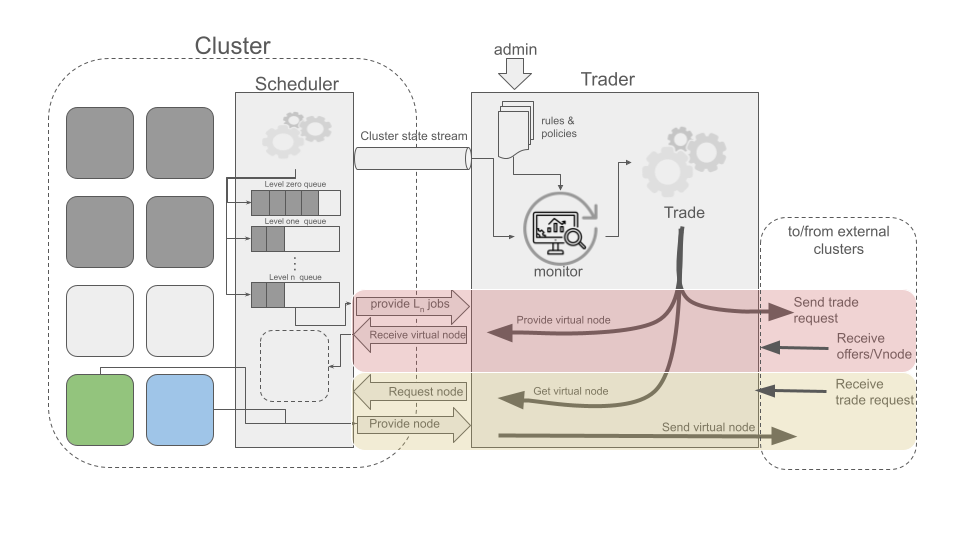
\includegraphics[scale=0.45]{figures/system-diagram}}
  \caption{System architecture showing the various compononents of the trader,
    and how it connects to a cluster. Red section represents the procedure
    requesting resources and the yellow section depicts the procedure of
    providing resources to external clusters. squares represents the node in
    the host cluster. Dark gray nodes represent localy utilized nodes and light
    gray nodes represent free local nodes. Green and blue nodes represent
    resources    provided to external clusters and the dotted square is a
    virtual node received from an external cluster} 
  \figlabel{fig1}
\end{figure}

\section{Scheduler}
% introducing the notion of minimal intursivity
\subsection{Requirements}
Cluster scheduling have been widely studied and remains a prominent area of
research. Our objective in relation to scheduling is not to replace the
clusters' scheduling algorithm nor interfere with its scheduling decisions, but
to improve the cluster's performance while minimizing friction and interaction
with the trader. It it also worth noting that the scheduler does not directly
interact with the broader multi-cluster environment but only with its own
trader, reducing the communication surface area and keeping local scheduling
independent from the mechanism. [NEEDS BETTER WORDING]

The scheduler's role in the mechanism comprises of passing on cluster state to
local trader, providing resources for trades, and receiving resources from
trades. Cluster state are measurements necessary to inform trading decisions.
These metrics are typically collected in cluster schedulers for performance
analysis and monitoring and include wait time, cost of compute/memory,
utilization etc.

\noindent Providing and receiving resources are an extension of the cluster's
ability to add new nodes and allocate resources on existing ones. 

Thus scheduling is detached from trading and only an interface is required to
connect the two modules together, allowing any scheduling algorithm already
running in a cluster to remain unchanged. This lays the ground to the general
requirements for a scheduler to operate in the mechanism, and shows that a
specific scheduling algorithm is not required for our mechanism. With that
being said, we now present our scheduling algorithm and discuss the underlying
design decisions. 

\subsection{Design}
% delay scheduling 

The base of our scheduling algorithm is delay scheduling [CITE] due to its
simplicity and []focus on data locality. In delay scheduling, a job is first
assigned the lowest level 0, allowing it to only be scheduled on the node its
data is at. The job is subsequently bumbed to higher levels as it fails to get
it scheduled in close proximity, permitting the scheduler to schedule the job
further away from its data as the wait time of the job increases. Consequently
the leveling represent the job's expectated distance from its data. This notion
of proximity and gradual drifting[] is extended to include external clusters in
our mechanism. Jobs already anticipating poor data locality would be the ones
more likely to be scheduled on an external cluster. This insures fair
scheduling even as we extend the scope of scheduling to a multi-cluster
environment. These jobs would also incur the least percentage reduction in
performance when scheduled in a foreign cluster.

\figref{fig1} includes the architecture of the scheduler described here. The
different queues represent different levels a job can be in. The incoming and
outgoing arrows represents the exposed interface the trader utilize to
communicate with the scheduler and will be further explained next.

%Of course, more analysis could go in deciding what jobs would better fit being
%exported to other clusters like jobs demanding less communiication with other
%jobs in the cluster, jobs with less data dependency, ..., but this is out of
%scope of this thesis.


% research idea: data locality-aware scheduling research is trying to get the
% jobs scheduled next to data, no study i encountered actually socres the
% sensitivity of the jobs in relation to other jobs in the cluster. (probably
% for fairness concerns) but might be an interesting project to work on. 

%This presents us with a clean heuristic when calculalting resources needed for
%trading. As the level of the of what to include in our 


\section{Trader} \label{trader}

The trader is the central component of the mechanism. It facilitates the
exchange of resources between clusters and encapsulates all trading logic. 

This exchange is bidirectional, meaning a cluster can receive external
resources and give away its own resources to other clusters. Clusters only
communicate with each other through their traders, which gets configured by the
cluster adminstrator. 

The trader is responsible for keeping the cluster's state in conformity with a
desired state. As shown in the figure, the trader establishes a cluster state
stream with the scheduler, continously sending up-to-date cluster information.
It includes the overall utilization, average job completion time, and current
cost of resources. This stream allows the trader to monitor the cluster state
and make trading decisions based on the current state of the cluster.

We will first examine what happens when the cluster needs resources, marked in
red in figref{fig1} and detailed in the following algorithm.

% Example Algorithm
\begin{figure}[H]
\begin{algorithm}[H]
\caption{Outgoing Trading Algorithm}
\begin{algorithmic}
  \Procedure{Trade}{$R_b$} \Comment{$R_b$ = broken rule}
    \State $R_{action} \gets Action(R_b)$
    \State $level_N Jobs \gets GetJobs(n)$ \Comment{get from scheduler}
    \State $virtualNodeSize \gets calculateNodeSize(R_{action}, level_N Jobs)$
    \For{traders in multi-cluster environment}
      \State $contract \gets SendTradeRequest(virtualNodeSize)$
    \EndFor
    \State $contracts \gets ReceiveTradeResponses$ \Comment{list of approved contracts}
    \State \textbf{return} $contract_{best}$\Comment{best virtual node is sent to scheduler}
  \EndProcedure
\end{algorithmic}
\end{algorithm}
\caption{Outgoing Trading Algorithm}
\end{figure}

The desired state is declared through a set of rules, which are
configurations dynamically passed to the trader shown below:  

\begin{figure}[H]
  \begin{lstlisting}[language=go]
    type Rule struct {
      Condition: // desired state to maintain
      Action: // algorithm to use
      Broken(cluster state, condition) bool
    } 
  \end{lstlisting}
  \caption{Rules}
\end{figure}

The rule's condition represents the desired value of a measurement sent by the
scheduler to the trader like utilization below 80\%. The rule implements a
Broken method which allows the trader to run an action when the actual cluster
state differs from the desired state. As the trader continously monitors the
cluster state, it runs the broken methods of all rules to check whether any is
broken. When a rule is broken, the trader's first step is to calculate the
resources it needs to request from other traders. To do that, it first requests
the last level jobs from the scheduler, resembling the jobs that would already
be scheduled further away from their data. The trader consults the broken rule
again, where the action variable specifies how to estimate the needed
resources. 

There are currently two ways to estimate the resource request: 
\begin{enumerate}

  \item \textbf{Optimized:} A greedy approach that stacks jobs efficiently over
    time on the requested node.

  \item \textbf{Take All:} Calculates resources as if all is scheduled at time
    0 on the requested node.

\end{enumerate}

The first approach allows the trader to reduce the size of the request which in
turn increases the chances of it getting approved, whereas the other approach
eagerly tries to increase the benefit from a trade.

After estimaing the needed resources, the trader then broadcasts a contract to
all participating clusters, and waits for replies. After receiving approved
contracts, the trader approves the best contract, and receives the virtual node
information from the foreign trader. It then sends the virtual node for the
scheduler to start scheduling jobs on it.

The trader is also responsible for accepting/rejecting incoming requests.
Outlined in the blue section of figure one and detailed in the following
algorithm: 

\begin{figure}[H]
\begin{algorithm}[H]
\caption{Incoming Trading Algorithm}
\begin{algorithmic}
  \Procedure{Trade}{$T_{request}$} \Comment{$T_{request}$ = trade request}
    \For{$P_{incoming}$ in Incoming policies}
      \If{$P_{incoming}(ccs, T_{request}) \not= true$} \Comment{ccs = current cluster state}
      \State \textbf{return} $false$ \Comment{Could not approve trade}
      \EndIf
    \EndFor
    \State $virtualNode \gets getVirtualNode(T_{request})$ \Comment{from scheduler}    
    \State \textbf{return} $virtualNode$ \Comment{Trade Approved}
  \EndProcedure
\end{algorithmic}
\end{algorithm}
\caption{Incoming Trading Algorithm}
\end{figure}

After receiving a contract request, the trader consults the incoming policy and the
current cluster state, and decides whether to approve the contract. If the
trader gets picked by the foreign cluster, the trader then requests the needed
resources from the scheduler and sends the node information back to the foreign
trader.

% add trading request algorithm

%The user defined outgoing policy also dictates any additional constraints the
%trader is required to adhere to. If the notion of a currency is established in
%the multi-cluster environmnet, constraints would include a budget, as well as a
%maximum price to pay for resources, which can be the price of renting out the
%resources from the vendor, or a cost estimate anaylsis algorithm. 

% rules intro
%A desired state is the state the orchestrator works on acheiving and keeping. A
%cluster adminstrator passes the desired state to the orchestrator, which in
%turn continously checks the actual state and compares it to the desired state
%while trying to restore the actual state to the desired one when it deviates.
%For example, if the desired state of a job on the cluster is having 3 replicas,
%and one server crashes, deleting one of the job's replicas, the orchestrator
%finds another healthy server to run the job's third replica on.  


%the conditions under which the the cluster begins requesting resources from
%external clusters.
% policies intro
\begin{figure}[H]
  \begin{lstlisting}[language=go]
    type Policy struct {
      Name  string
      Conditions // cluster state that allows approval
      Incentive // offer from external cluster
      ApproveRequest(request) bool 
    } 
  \end{lstlisting}
  \caption{Custom Policy implements an approveRequest method}
\end{figure}
Policies are asymmetrical to rules, in that they dictate how the trader
responds to received resource requests.

%Both rules and policies act as knobs to tune the mechanism and update it as
%cluster state and requirements change. They are pluggable and mutable, meaning
%each cluster admin can implement their own and dynamically update them as
%cluster requirements and conditions change.
%
%The metrics in scope are the ones sent by the scheduler, and include wait time,
%job completion time, utilization, cost, etc. 
%
%We design both rules and policies as interfaces, enabling them to
%be pluggable and user-defined. Policies implement an
%\texttt{approveRequest()} method, which returns true when an external trader's
%request is feasible, where as rules implement a \texttt{Broken()} method
%signature, triggering the trader to request resources when the cluster state
%breaks the conditions.  
%
%A cluster admin aiming to reduce wait time would create a rule that breaks when
%average wait time exceeds the specified threshold, and a policy that refuses to
%provide resources under similar conditions. Optimizing for utilization, an
%admin would create a rule that breaks when utilization surpasses a resource
%utilization threshold and a policy that denies resources for the same
%criterion. Tuning the policies as requirements change can be achieved by
%increasing or decreasing the respective thresholds. Stopping all trading rules
%and policies is another way to adjust the mechanism. An admin might disable
%policies altogether during peak times to enhance system predictability. 

% TRADER SECTION START

%Our mechanism offers bidirectional trading, allowing clusters to trade
%resources with one another. It also enables trading with multiple clusters, so
%clusters can trade resources with more than one cluster at a time.
%\label{sched-overhead} The following algorithms show a simple representation
%of the system, with resource utilization as the optimized-for metric:
%\label{example}

%%% -*-LaTeX-*-

\chapter{Implementation} 

In the previous section, we outlined the theoretical design of the system. This
section goes over the implementation of the simulator written to evaluate the
mechanism.

%Why simulator 
We decided that having a simulator will allow us a broader scope for testing
the trading mechanism. Although it is possible to build the mechanism on top of
current multi-cluster networking solutions, we will be limited to the design
decisions of the tools used. Having a broader simulated results will open the
door for more interesting questions and answers leading to a concrete system
being built on an actual cluster.

The simulator is implemented as a set of seperate Go packages that can be run
in a distributed fashion.
\begin{enumerate}
  \item Trader: main module responsible for the functionality of the mechanism
  \item Scheduler: responsible for scheduling jobs on the cluster,
    communicating cluster state with the trader, providing/receiving virtual
    nodes 
  \item Client: Imports production traces or creates synthetic workloads and
    sends it to the schedueler.
\end{enumerate}

The simulator also includes other bookkeeping components like a service package
and a registry that don't interfere much with the evaluation and won't be
further discussed.

The client communicates with the scheduler through http, whereas as the
scheduler-trader and trader-trader communication is through grpc. 

\section{Scheduler} 

This section only discusses design decisioins and additions made relating to
the mechanism. These components are on top of regular scheduling functionality. 

The main aspect to be discussed in the scheduler is the scheduling algorithm
itself. It is a two level delay scheduling algorithm. A job is first added to
level 0 queue, and sent to level 1 queue if not scheduled in X time. Level 1
jobs are more likely to be scheduled away from their data, hence these are the
ones that will be sent to the trader when estimating the size of the node to
send. A distinctive difference to the delay scheduling algorithm is that the
nodes do not request jobs to be scheduled on them, but instead the scheduling
algorithm looks for nodes to schedule the jobs, similar to widely used cluster
schedulers.

A node burst scheduling is also implemented in the scheduler. Once a virtual
node is added to the cluster, the cluster tries to schedule as much viable jobs
it can on it right away to increase utilization of the virtual node, since the
node have a deadline. 

The scheduler also implements a gRPC server responsible for sending the
required cluster state to the trader.

\section{Trader}

The trader receives the cluster state from the scheduler through a continious
loop as a gRPC client. The trader then runs a state monitor, cycling through
the outgoing policies to check whether any is broken.   

\subsection{Trading algorithm}

When cluster state breaks a policy, trading is initaited. The trader retrieves
a list of active traders from the regisrty, estimates the amount of resources
needed while abiding to constraints, and sends a contract request to all
participating traders. It then chooses the most favorable trader, approves the
contract, and adds the received virtual node to the local cluster. 

\subsection{Policies}

\lstinputlisting[language=go, firstline=94,
lastline=96]{../multi-cluster-simulator/pkg/trader/trader.go}

The outgoing policies are implemented as an interface with a Broken method
signature. This allows the policies to be pluggablle. The user can define the
policy as long as there's a notion that the policy can break depending on the
cluster changes.

We currently implement two Policies:
\begin{enumerate}
  \item Wait time: The policy is broken if the average wait time in the cluster
    is above a threshold.
  \item Utilization: The policy is broekn if resource utilization exceeds a
    limit. 
\end{enumerate}

Incoming policies do not have the pluggibility trait. Users dial the knobs for
accepting incoming contracts with respect to the cluster state.

\chapter{Evaluation}

This section presents a comprehensive evaluation of the proposed trading
mechanism, focusing on its performance, scalability, and overall effectiveness
in multi cluster environments. We employ a combination of synthetic and
real-world workloads to simulate various scenarios, alongside an array of rules
and policies to investigate beneficial strategies and the effectiveness of
different workload-strategy combinations.

However, the possible combinations of rules, policies and their respective
configurations is infinite. Our aim in this section is not to exhaust all
possibilities, but to explore the validity of the mechanism under different
constraints. This approach paves the way for users to conduct their experiments
on thier specific workloads to determine the strategy that best fits their
needs.  

All experiments are run on Cloudlab, a scientific infrastructure used by
academics for systems and cloud research \cite{duplyakin_design_2019}. We
utilize the following setups to to run the experiments. Each node in the setups
simulates one cluster, with the cluster, trader, and client running on the same
machine. 
% CITE CLOUDLAB NODES
\begin{enumerate}

  \item \textbf{Setup One:} 3 Cloudlab nodes c6525-100g running Linux
    Ubuntu 22.04 in the same Utah datacenter. Cluster sizes are equal having 10
    nodes each with 32 cores and 24GBs of memory.

  \item \textbf{Setup Two:} 3 Cloudlab nodes of type m510, c220g1, c8220
    running on three distinct datacenters in Utah, Wisconsin, and Clemson, and
    have the same cluster sizes as those in Setup One.

\end{enumerate}

The setups simulate different scenarios where clusters can belong to one
organization or different organizations, and have varying network latency and
bandwidth.  

We derive our results by running a configuration of rules, policies, and
workloads twice, once with and once without the mechanism and compare the
performance difference.

Our methodology for running workloads is as follows: All participating clusters
have the same start and end time for receiving jobs from their respective
clients. After the clients stop sending jobs, the experiment is kept on until
the last job in the slowest cluster finish execution. 

\section{Experiment One}

\begin{center}
  \fbox{\parbox{14cm}{
  
    \underline{Configuration:}
    \vspace{.3em}
    \begin{enumerate}
  
      \item \textbf{Setup:} \#1 with three cooperative clusters.
  
      \item \textbf{Workload:} Synthetic, all clusters are oversubscribed.
      
      \item \textbf{Rules:} Approve trades if average wait time is below 5
        seconds and both memory and core utilization below 0.8
      
      \item \textbf{Policies:} Initiate trades if utilization is above 0.8 or
        average wait time above 60 seconds.
  
    \end{enumerate}
  }}
\end{center}
We will first examine the scenario where all cooperative clusters have high
resource utilization for the entirety of the experiment duration.

%We aim by this experiment to showcase the overhead of the trading mechanism
%where it's likely not beneficial to participate.

\begin{figure}[H]
\centering
\begin{subfigure}{.5\textwidth}
  \centering
  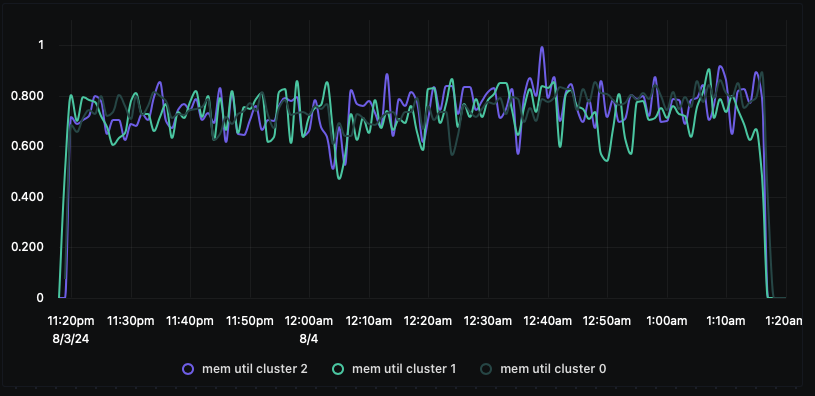
\includegraphics[width=.9\linewidth]{./figures/experiment-one/cooperative-clusters-all-at-100-trading-mem-util.png}
  \caption{cooperative clusters}
  \label{fig:exp1coop}
\end{subfigure}%
\begin{subfigure}{.5\textwidth}
  \centering
  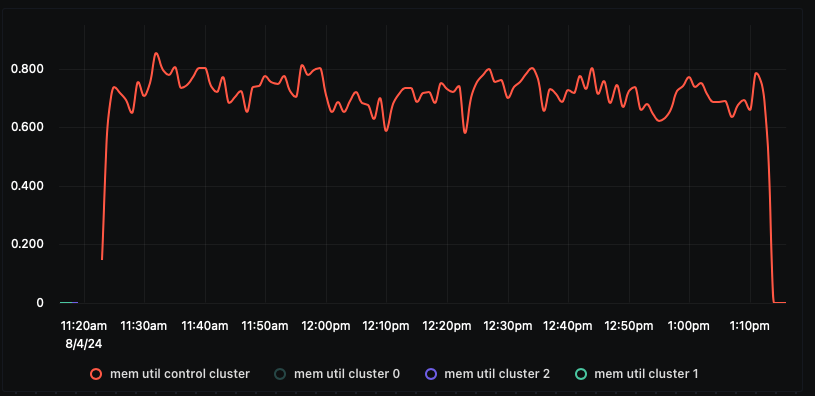
\includegraphics[width=.9\linewidth]{./figures/experiment-one/control-mem-util.png}
  \caption{control cluster}
  \label{fig:exp1control}
\end{subfigure}
\caption{Experiment 1, memory utilization}
\label{fig:exp1memutil}
\end{figure}

Figure~\ref{fig:exp1memutil} presents the memory utilization of the cooperative
clusters in \ref{fig:exp1coop} and the same workload run on a cluster without
trading in \ref{fig:exp1control}.
% analysis
We can see that the control cluster have a slightly lower utilization averaging
at 70\% whereas cooperative clusters' memory utilization averaged at 75\%. This
5\% difference is due to cooperative clusters doing quick trades during short
downtime intervals, leading to an inefficient scheduling and coupled with
higher utilization. In this case, trading is discouraged or a higher buffer
between trades is preferred. We can draw the same conclusion for the difference
in core utilization with 65\% and 71\%. However, this led to a 5.45\% increase
in total time to finish all jobs as local resources were occationally lent
just before a spike in jobs, delaying the execution of the local ones. As this
phenomenon happened on all clusters, they all suffered decreased performance.
It's important to mention that a cluster can't evict external allocations once
the contract is approved, hence a trade can be expensive without proper
considerations.

We can see this effect play out in the number of jobs in the scheduler's queues.
\begin{figure}[H]
  \begin{center}
    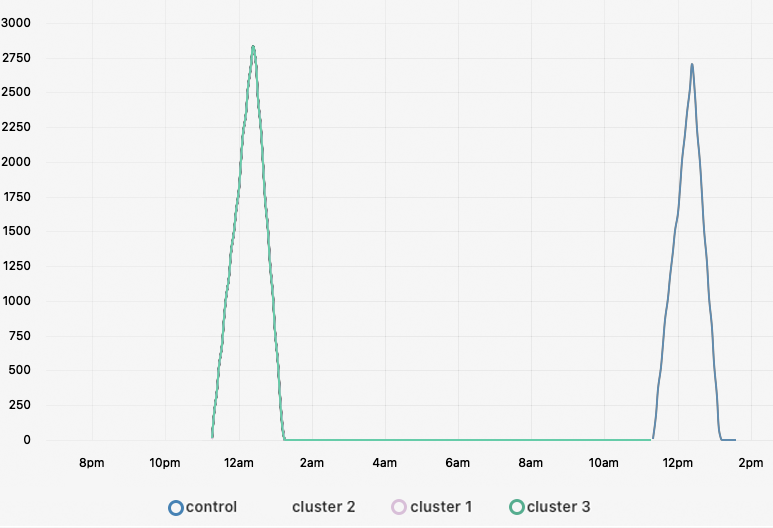
\includegraphics[width=0.5\textwidth]{./figures/experiment-one/jobs-in-queue.png}
  \end{center}
  \caption{}\label{fig:exp-1-jobs-in-queue}
\end{figure}

As seen in figure~\ref{fig:exp-1-jobs-in-queue}, all participating
clusters incurred an increased number of jobs in the queue at the peak. Note
that the peak is created because of our workload methodology. The decreasing
part of the graph resembles the cool down time, or the time it takes to finish
scheduling all jobs after the client is done sending them. As all these clusters
are oversubscribed; jobs keep getting queued until the client is done 
sending. The total workload per cluster in this experiment was around 8000
jobs. 

\section{Experiment Two}

\begin{center}
  \fbox{\parbox{14cm}{
  
    \underline{Configuration:}
    \vspace{.3em}
    \begin{enumerate}
  
      \item \textbf{Setup:} \#1 with three cooperative clusters.
  
      \item \textbf{Workload:} Synthetic 
        \vspace{-.5em}
          \begin{enumerate}
            \item One underutilized. 
            \item One highly utilized. 
            \item One oversubscribed. 
          \end{enumerate} 
      
      \item \textbf{Rules:} Approve trades if average wait time is below 5
        seconds and both memory and core utilization below 0.8
      
      \item \textbf{Policies:} Initiate trades if utilization is above 0.8 or
        average wait time above 60 seconds.
  
    \end{enumerate}
  }}
\end{center}

In this experiment, we run trading on a similar rule and policy configuration
as experiment one but with varying workloads between clusters, detailed in the
configuration box above. 

\begin{figure}[H]
\centering
\begin{subfigure}{.5\textwidth}
  \centering
  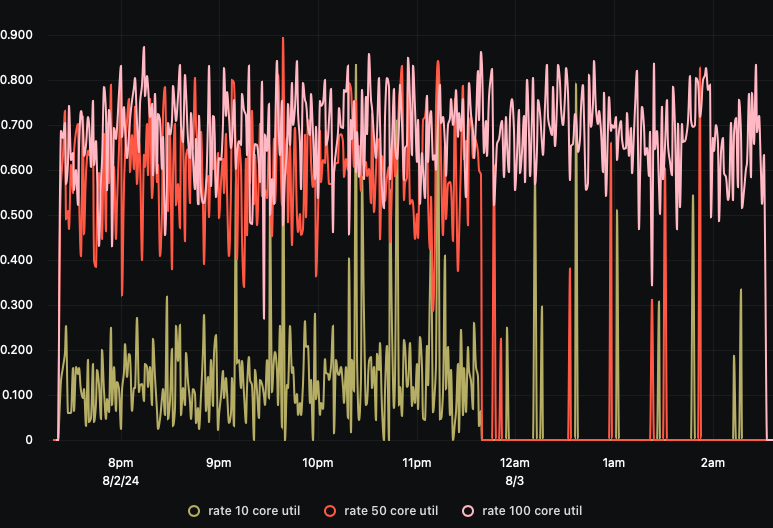
\includegraphics[width=.9\linewidth]{./figures/experiment-two/trading.png}
  \caption{cooperative clusters}
  \label{fig:exp2coop}
\end{subfigure}%
\begin{subfigure}{.5\textwidth}
  \centering
  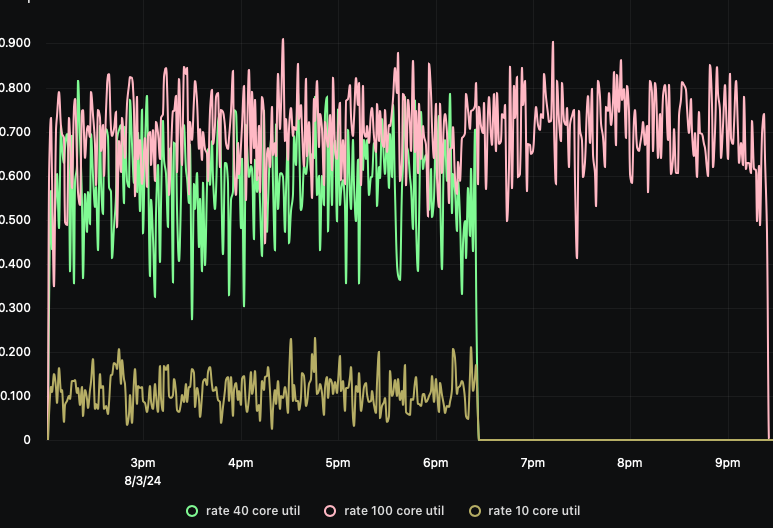
\includegraphics[width=.9\linewidth]{./figures/experiment-two/control.png}
  \caption{control cluster}
  \label{fig:exp2control}
\end{subfigure}
\caption{Experiment 2, core utilization}
\label{fig:exp2coreutil}
\end{figure}

Figure~\ref{fig:exp2coreutil} displays the core utilization of the cooperative
clusters in \ref{fig:exp2coop} and the same workload run on a cluster without
trading in \ref{fig:exp2control}.
% analysis
The first evident difference between the two graphs is the spikes seen on the
underutilized cluster and less apparent on the highly utilized. These
indicate the occurence of trades, benefiting the highly utilized 100
jobs/minute cluster. Trading did not negatively affect the performance of any
of the particpating clusters, and it decreased the total time to finish all jobs in
the environment by 5.8\%, from 7 hours and 28 minutes to 7 hours.

\section{Experiment Three}

\begin{center}
  \fbox{\parbox{14cm}{
  
    \underline{Configuration:}
    \vspace{.3em}
    \begin{enumerate}
  
      \item \textbf{Setup:} \#1 with three cooperative clusters.

      \item \textbf{Workload:} Synthetic
          \vspace{-.5em}
          \begin{enumerate}
            \item Two highly utilized clusters
            \item One small cluster with varying utilization levels 
          \end{enumerate} 
      \item \textbf{Rules:} Approve trades if average wait time is below 5
        seconds and both memory and core utilization below 0.8
      
      \item \textbf{Policies:} Initiate trades if utilization is above 0.8 or
        average wait time above 60 seconds.
  
    \end{enumerate}
  }}
\end{center}

This experiment models a scenario with some similarity to the machine learning
training-inference workloads the Lyra system takes advantage of
\cite{li_lyra_2023}, albeit with some differences. There are two big highly
utilized clusters, and one small cluster experiencing low utilization in
addition to spikes. We kept the rules and policies similar to the previous
experiments for reference. The figure below shows the memory utilization of
these clusters. 

\begin{figure}[H]
\centering
\begin{subfigure}{.5\textwidth}
  \centering
  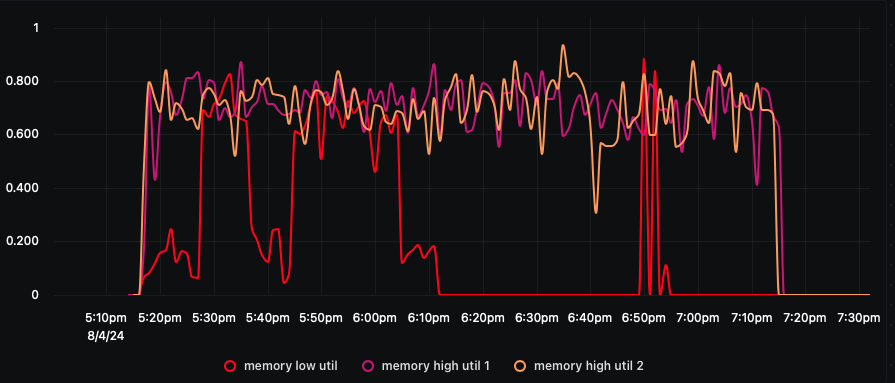
\includegraphics[width=.9\linewidth]{./figures/experiment-three/cooperative.png}
  \caption{cooperative clusters}
  \label{fig:exp3coop}
\end{subfigure}%
\begin{subfigure}{.5\textwidth}
  \centering
  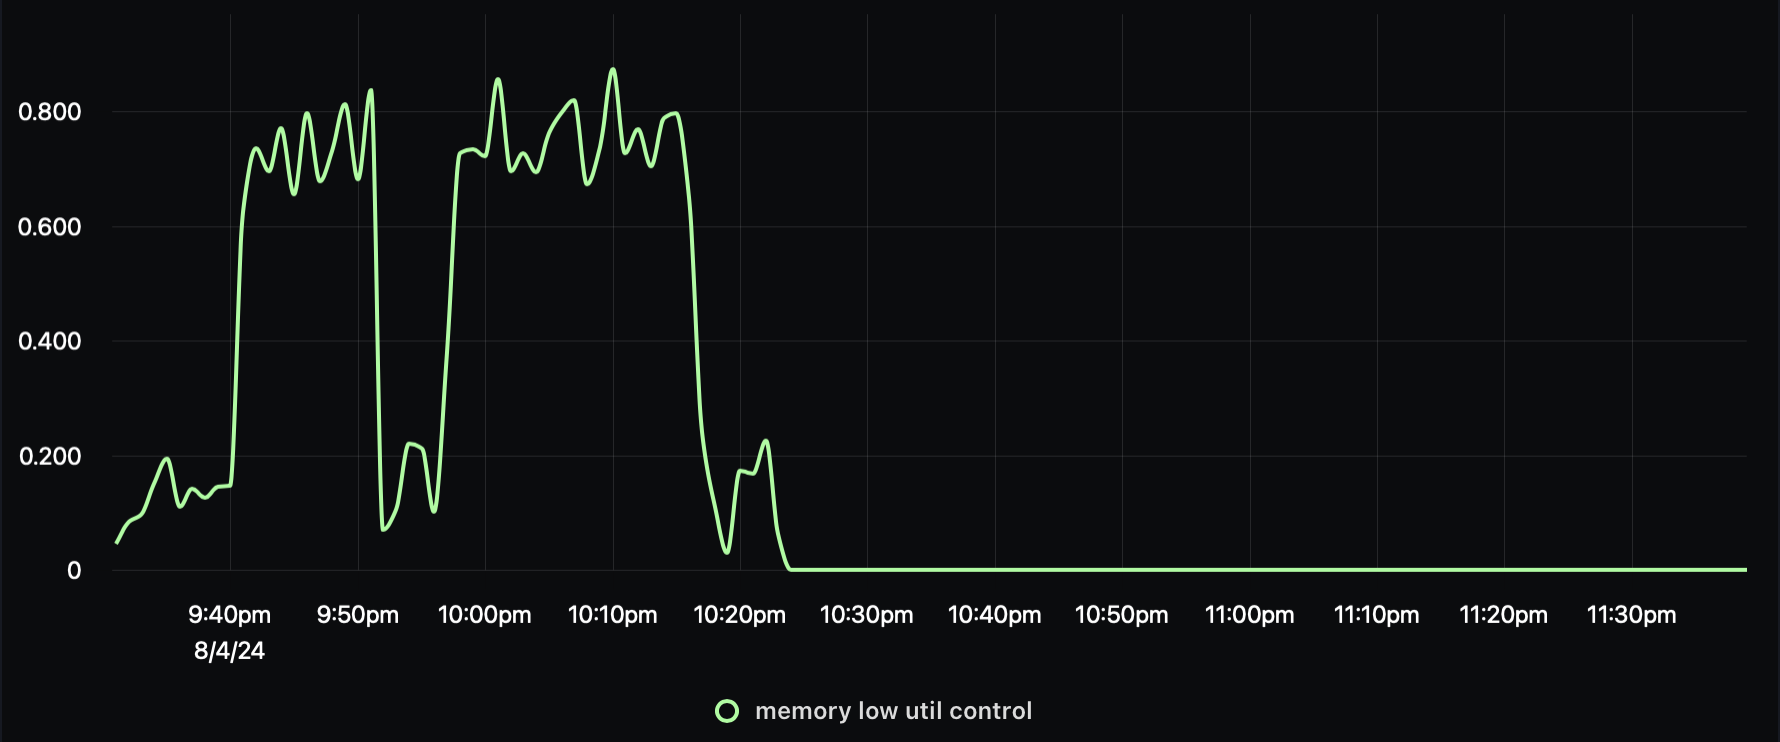
\includegraphics[width=.9\linewidth]{./figures/experiment-three/control.png}
  \caption{control cluster}
  \label{fig:exp3control}
\end{subfigure}
\caption{Experiment 3, memory utilization}
\label{fig:exp3memutil}
\end{figure}

The small cluster did not incur any degradation for loaning its resources, as
job completion time and total time to finish all jobs remained the same. The
highly utilized clusters were able to manage their workloads for most of the
experiment, with the small cluster experiencing only 15\% increase in
utilization. This led to a  4\% reduction in time to schedule all jobs in the
highly utilized clusters. 


%\section{Experiment Four}

% the goal is to test different policies and see which ones, coupled with the
% appropriate workload, achieves one of the goals stated in the thesis
% statement.
%\section{Limitations}
%
%- workload overfitting
%https://www.usenix.org/system/files/conference/atc18/atc18-amvrosiadis.pdf
%
%- simulation not actual system

%%% -*-LaTeX-*-

\chapter{Conclusion}

In this thesis, we explored the complexities of multi-cluster environments and
proposed a novel trading mechanism to address the challenges associated with
resource fragmentation, increased costs, and reduced resource utilization. 

Through simulated experiments, we have demonstrated that the mechanism can
improve cluster performance by increasing resource utilization, reducing costs,
and decreasing job wait times. We've also shown that this improvement is
dependendent on careful workload analysis. The trader should be fine-tuned
through rules and policies to accommodate the specificity of the cluster's
workload. 

With an extensible mechanism, trading between clusters can be generalized and
adapted to fit clusters' needs, providing a robust tool in the multi-cluster
space. 


%%% -*-LaTeX-*-

\chapter{Future Work}

Analysis on which jobs would better fit being exported
Work on estimating workload for node size requests
% https://www.usenix.org/system/files/nsdi22-paper-jajoo_5.pdf

Allow auctioning of resources to reduce cost:
% https://www.researchgate.net/publication/286098696_Auction_based_resource_allocation_in_cloud_computing

build the system on an actual cluster for better results
liqo


% \numberofappendices = 1   % Set 0 for none, else number of appendices.
%\numberofappendices = 3
%\appendix       % Chapters, sections are now appendix style A, A.1, A.2, B, C, D, ...
%
%%%% -*-LaTeX-*-

\chapter{The First}

This is an appendix.  Notice that the \LaTeX{} markup for an appendix
is, surprisingly, \verb=\chapter=.  The \verb=\appendix= command does
not produce a heading; instead, it just changes the numbering style
from numeric to alphabetic, and it changes the heading prefix from
\textbf{CHAPTER} to \textbf{APPENDIX}.

\blah \blah \blah

%%%% -*-LaTeX-*-

\chapter{The Second}

This is an appendix.

\blah \blah \blah

%%%% -*-LaTeX-*-

\chapter{The Third}

This is an appendix.

There are several books
\cite{%
    Singh:1997:FEE,%
    Salomon:1995:AT,%
    Robbins:2005:CSS,%
    Randell:1982:ODC,%
    Olver:2010:NHM,%
    Mittelbach:2004:LC,%
    Lamport:1985:LDP,%
    Knuth:1999:DT,%
    Knuth:1986:TB,%
    Knuth:1986:MB,%
    Farmelo:2009:SMH%
}
listed in our bibliography.

We also reference several journal articles
\cite{%
    Wiles:1995:MEC,%
    Taylor:1995:RTP,%
    Lahiri:2002:ADA,%
    Kim:1999:AFC,%
    Johnson:1978:LDT,%
    Huskey:1980:LLC,%
    Heilbron:1969:GBA,%
    Hall:1994:PNE,%
    Goldstine:1946:ENI,%
    Einstein:1911:BMAb,%
    Einstein:1911:BMAa,%
    Einstein:1906:NBM,%
    Cody:1981:APF,%
    Beebe:1989:PCP,%
    Babbage:1910:BBA%
}
and three famous doctoral theses of later winners
\cite{%
    Einstein:1905:NBM,%
    Dirac:1926:QM,%
    Bohr:1911:SME%
}
of the Nobel Prize in Physics (1922, 1933, and
1921):

Notice that, even though those citations appeared
in \LaTeX{} \verb=\cite{...}= commands with their
\BibTeX{} citation labels in reverse alphabetical
order, thanks to the \verb=citesort= package,
their reference-list numbers have been sorted in
numerically ascending order, and then
range-reduced.

Mention should also be made of a famous Dutch
computer scientist's first publication
\cite{Dijkstra:1953:FBV}.

Font metrics are an important, albeit low-level,
aspect of typesetting. See the \emph{Adobe
Systems} manual about that company's procedures
\cite{Adobe:1990:AFM}.

The bibliography at the end of this thesis contains several examples
of documents with non-English titles, and their \BibTeX{} entries
provide title translations following the practice recommended by the
American Mathematical Society and SIAM\@.  Here is a sample entry that
shows how to do so:
%
\begin{verbatim}
@PhdThesis{Einstein:1905:NBM,
  author =       "Albert Einstein",
  title =        "{Eine Neue Bestimmung der Molek{\"u}ldimensionen}.
                 ({German}) [{A} new determination of molecular
                 dimensions]",
  type =         "Inaugural dissertation",
  school =       "Bern Wyss.",
  address =      "Bern, Switzerland",
  year =         "1905",
  bibdate =      "Fri Dec 17 10:46:57 2004",
  bibsource =    "http://www.math.utah.edu/pub/tex/bib/einstein.bib",
  note =         "Published in \cite{Einstein:1906:NBM}.",
  acknowledgement = ack-nhfb,
  language =     "German",
  advisor =      "Alfred Kleiner (24 April 1849--3 July 1916)",
  URL =          "http://en.wikipedia.org/wiki/Alfred_Kleiner",
  remark =       "Received August 19, 1905 and published February 8,
                 1906.",
  Schilpp-number = "6",
}
\end{verbatim}

The \texttt{note} field in that entry refers to another bibliography
entry that need not have been directly cited in the document text.
Such cross-references are common in \BibTeX{} files, especially for
journal articles where there may be later comments and corrigenda that
should be mentioned.  Embedded \verb=\cite{}= commands ensure that
those possibly-important other entries are always included in the
reference list when the entry is cited.  The last bibliography entry
\cite{Wiles:1995:MEC} in this thesis has a long \texttt{note} field
that tells more about what some may view as the most important paper
in mathematics in the last century.

When entries cite other entries that cite other entries that cite
other entries that \ldots{}, multiple passes of \LaTeX{} and \BibTeX{}
are needed to ensure consistency.  That is another reason why document
compilation should be guided by a \texttt{Makefile} or a batch script,
rather than expecting the user to remember just how many passes are
needed.

\BibTeX{} entries are \emph{extensible}, in that arbitrary key\slash
value pairs may be present that are not necessarily recognized by any
bibliography style files.  The \texttt{advisor},
\texttt{acknowledgement}, \texttt{bibdate}, \texttt{bibsource},
\texttt{language}, \texttt{remark}, and \texttt{Schilpp-number} fields
are examples, and may be used by other software that processes
\BibTeX{} entries, or by humans who read the entries.  \texttt{DOI}
and \texttt{URL} fields are currently recognized by only a few styles,
but that situation will likely change as publishers demand that such
important information be included in reference lists.

In \BibTeX{} \texttt{title} fields, braces protect words, such as
proper nouns and acronyms, that cannot be downcased if the selected
bibliography style would otherwise do so.  In German, all nouns are
capitalized, and the simple way to ensure their protection is to brace
the entire German text in the title, as we did in the entry above.

The world's first significant computer program may
have been that written in 1842 by Lady Augusta Ada
Lovelace (1815--1852) for the computation of Bernoulli
numbers \cite{Huskey:1980:LLC,Kim:1999:AFC}.  She
was the assistant to Charles Babbage
(1791--1871), and they are the world's first
computer programmers. The programming language
\emph{Ada} is named after her, and is defined in
the ANSI/MIL-STD-1815A Standard; its number
commemorates the year of her birth.

We do not discuss mathematical \emph{transforms}
in this dissertation, but you can find that phrase
in the index (except that this sample thesis doesn't have one!)

\blah

\blah
\blah

\blah


%%% The choice of bibliography style is a major decision, jointly made
%%% by you, your thesis advisor and the thesis editor. Common choices are
%%% one of the four standard BibTeX styles (abbrv, alpha, plain, and unsrt),
%%% or enhanced styles like acm, amsplain, siam, and hundreds of others
%%% available in TeX Live, and other Unix and Windows TeX distributions.
%%%
%%% Do NOT handcode your reference list, because you are unlikely to
%%% achieve consistency or conformance to the University of Utah Thesis Office
%%% requirements: let BibTeX do that tedious job for you!
%%%
%%% Remember that reference-list metadata in BibTeX files remains
%%% constant across journals and publishers, and is are often reused
%%% in other documents and shared with others, whereas formatted
%%% reference-list styles change: with BibTeX, you only need to record
%%% the metadata once.
%%%
%%% If you prefer named, rather than numeric or tagged citations, you
%%% may use styles such as authordate{1,2,3,4}, chicago, harvard, or
%%% natbib.  Be aware, however, that most of those require an
%%% additional \usepackage{} command to supply \LaTeX{} with
%%% definitions of commands that the style needs, and that there are
%%% usually several flavors of LaTeX citation commands beyond the
%%% standard \cite{} command that you need to understand before you
%%% can use them properly in your prose.

%%% This tells BibTeX to read siam.bst from the first directory where
%%% it is found in the BSTINPUTS search path:

\bibliographystyle{siam}

%%% This can also specify a comma-separated list (without embedded
%%% spaces) of *.bib files found by BibTeX in its BIBINPUTS search
%%% path.  The argument \jobname means the base name of the top-level
%%% LaTeX file, avoiding an unnecessary filename dependence here.
%%%
%%% BibTeX writes only one .bbl file, no matter how many *.bib files
%%% are listed here, using the name \jobname.bbl.
%%%
%%% LaTeX reads BibTeX's formatted reference list from the file
%%% \jobname.bbl.

\bibliography{proposal}

\end {document}
